\documentclass[mathserif]{beamer}
\usepackage{beamerthemeshadow}
\usepackage{beamerthemesplit}
%\usetheme{shadow}
\usecolortheme{default}
\setbeamertemplate{footline}[frame number]
\useinnertheme[shadow=true]{rounded}
%\setbeamertemplate{footline}{\insertframenumber/\inserttotalframenumber}
%\useoutertheme{infolines}
%\setbeamertemplate{headline}{} % removes the headline that infolines inserts

%\usetheme{boxes}
%\usepackage{amsmass}
%\usepackage{amssymb,amsfonts,url}
\usepackage{multirow}

\usepackage{algorithm}
\usepackage{algorithmic}
 
\usepackage{graphicx}
\graphicspath{{Problems/}}
\usepackage{verbatim}

\usepackage{tikz}
\usetikzlibrary{shadows}
\usepackage{verbatim}
\usepackage{pgfplots}
\usepackage{verbatim}
\usetikzlibrary{arrows,shapes}

\definecolor{darkblue}{rgb}{0.2,0.2,0.6}
\definecolor{darkred}{rgb}{0.6,0.1,0.1}
\definecolor{darkgreen}{rgb}{0.2,0.6,0.2}

\usetikzlibrary{shadings,shadows,shapes.arrows}

\usetikzlibrary{calc} 

\tikzstyle{vertex}=[circle,fill=black!25,draw,minimum size=20pt,inner sep=0pt]
\tikzstyle{middlevertex}=[circle,fill=black!25,draw,minimum size=15pt,inner sep=0pt]
\tikzstyle{smallvertex}=[circle,fill=black!25,draw,minimum size=10pt,inner sep=0pt]
\tikzstyle{selected vertex} = [vertex, draw,fill=red!24]
\tikzstyle{blue smallvertex} = [smallvertex, draw,fill=blue]
\tikzstyle{red smallvertex} = [smallvertex, draw,fill=red]
\tikzstyle{edge} = [draw,thick,->]
\tikzstyle{undirectededge} = [draw,thick]
\tikzstyle{weight} = [font=\small]
\tikzstyle{selected edge} = [draw,line width=5pt,-,red!50]
\tikzstyle{ignored edge} = [draw,line width=5pt,-,black!20]

%\usepackage{CJK}
%\usepackage{pinyin}

%    \begin{figure}
%        \centering
%        \includegraphics[width=0.8\textwidth]{newGeneRep.eps}
%    \end{figure}

% \begin{figure}%
%   \begin{center}%
%     \begin{minipage}{0.70\textwidth}%
%      \includegraphics[width=1.0\textwidth]{comp25000.eps}%
%     \end{minipage}%
%     \begin{minipage}{0.30\textwidth}
%      \includegraphics[width=1.0\textwidth]{comparelabel.eps}%
%     \end{minipage}%
%   \end{center}
% \end{figure}

% \begin{table}
%   {\begin{tabular}{l|rrr}\hline
%       & \multicolumn{3}{c}{Actual number of DCJ operations}\\
%       \# genes &\# genes $\times 1$&\# genes $\times 2$&\# genes  $\times 3$ \\
% \hline
%      (a)~25,000 & 0.5\% ~~&  0.9\% ~~& 1.7\%~~\\
%       (b)~10,000 & 0.8\%~~ &  1.4\% ~~& 2.7\%~~\\
%      (c)~ 1,000 & 2.7\%~~ & 4.7\%~~ & 14.7\%~~\\ \hline
%     \end{tabular}} {}%
% \end{table}

% \begin{eqnarray}
% T(n) &=&  \sum_{i=1}^n C_i \\
%      &=&  \# PUSH + \#POP \\
%      &<& 2\times \#PUSH \\
%      &<& 2n \\
% \end{eqnarray}

% \[ 
% \begin{matrix}
% \begin{pmatrix}
% C_{11} & C_{12} \\ 
% C_{21} & C_{22} 
% \end{pmatrix}
% =
% \begin{pmatrix}
% A_{11} & A_{12} \\ 
% A_{21} & A_{22}  
% \end{pmatrix}
% 
% \begin{pmatrix}
% B_{11} & B_{12} \\ 
% B_{21} & B_{22}  
%  
% \end{pmatrix}
%     
%    \end{matrix}
% \]
% 
% 
% \begin{eqnarray}
%  C_{11} &=& (A_{11}\times B_{11}) + (A_{12} \times B_{21}) \\
% C_{12} &=& (A_{11}\times B_{12}) + (A_{12} \times B_{22}) \\
% C_{21} &=& (A_{21}\times B_{11}) + (A_{22} \times B_{21}) \\
% C_{22} &=& (A_{21}\times B_{12}) + (A_{22} \times B_{22}) 
% \end{eqnarray}
% \begin{figure}%
%      \begin{minipage}{0.32\textwidth}%
%       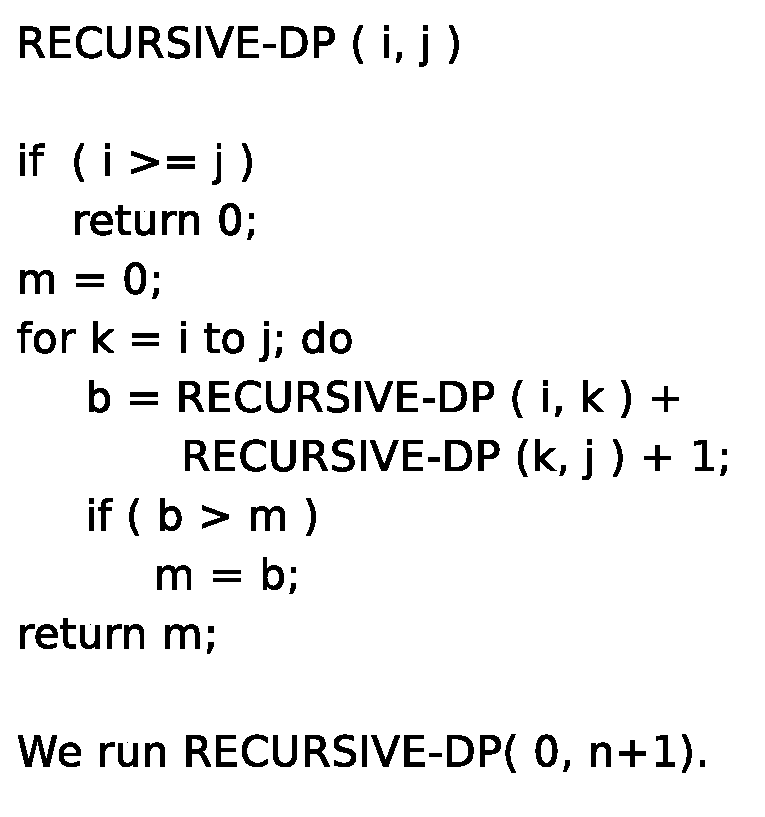
\includegraphics[width=1.0\textwidth]{L7-intervalschedulingdpalgo.eps}%
%      \end{minipage}%
%  \quad
%      \begin{minipage}{0.30\textwidth}
%       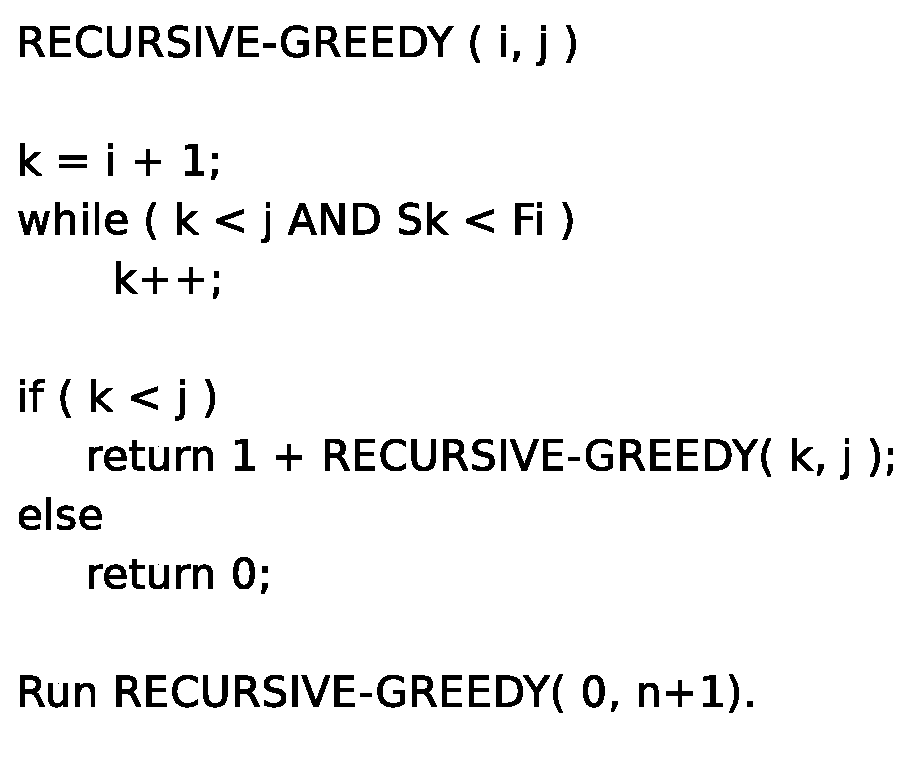
\includegraphics[width=1.0\textwidth]{L7-intervalschedulinggreedyalgo.eps}%
%      \end{minipage}%
%  \quad
%       \begin{minipage}{0.25\textwidth}
%       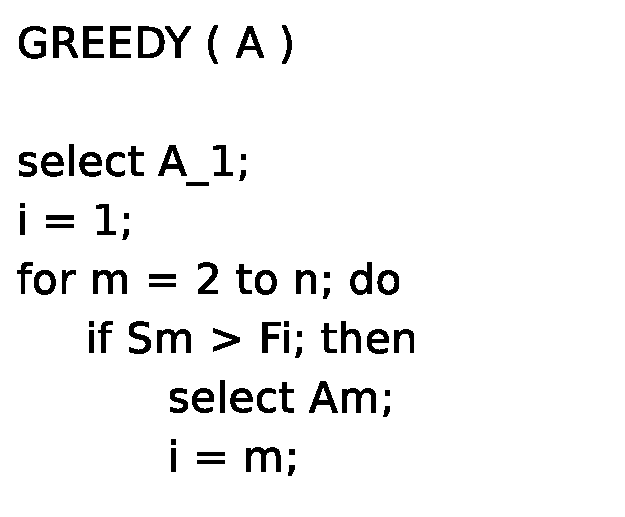
\includegraphics[width=1.0\textwidth]{L7-intervalschedulinggreedyalgo2.eps}%
%      \end{minipage}%
% 
%  \end{figure}

\title{CS711008Z  Algorithm Design and Analysis }
\subtitle{ Lecture 9. Lagrangian duality and SVM 
%\footnote{The slides were made based on Ch 29 of Introduction to algorithms, Combinatorial optimization algorithm and complexity by C. H. Papadimitriou and K. Steiglitz. } 
}
\author{Dongbo Bu } 
\institute{ {\small Institute of Computing Technology \\ 
Chinese Academy of Sciences, Beijing, China}}

\date{}
\begin{document}
%\begin{CJK}{UTF8}{cyberbit}
\frame{\titlepage}

\frame{
\frametitle{Outline}
\begin{itemize}
	\item Classification problem and maximum margin strategy; 
	\item Solving maximum margin problem using Lagrangian duality; 
	\item SMO technique; 
	\item Kernel tricks; 
\end{itemize}
} 

%\frame{
%\frametitle{}
%Remarks: 
%
%
%\begin{enumerate}
% \item \textcolor{red}{When minimizing a function $f(x)$, it is valuable to know a lower bound of $f(x)$ in advance.} 
% \item Knowing lower bound is important to approximation algorithm, and {\it branch-and-bound} technique. 
% %EM is an example to maximize a lower bound rather than the objective function itself.  }
% \item \textcolor{red}{Duality} and relaxation are powerful techniques to set a reasonable lower bound.
% \item Linear programs come in primal/dual pairs. 
% \item It turns out that every feasible solution for one of these two problems provides a bound for the objective value for the other problem. 
%\end{enumerate}
%}

\frame{
\begin{block}{}
	 Classification problem and maximum margin strategy
\end{block}
}

\frame{
\frametitle{Classification problem}

\begin{figure}
   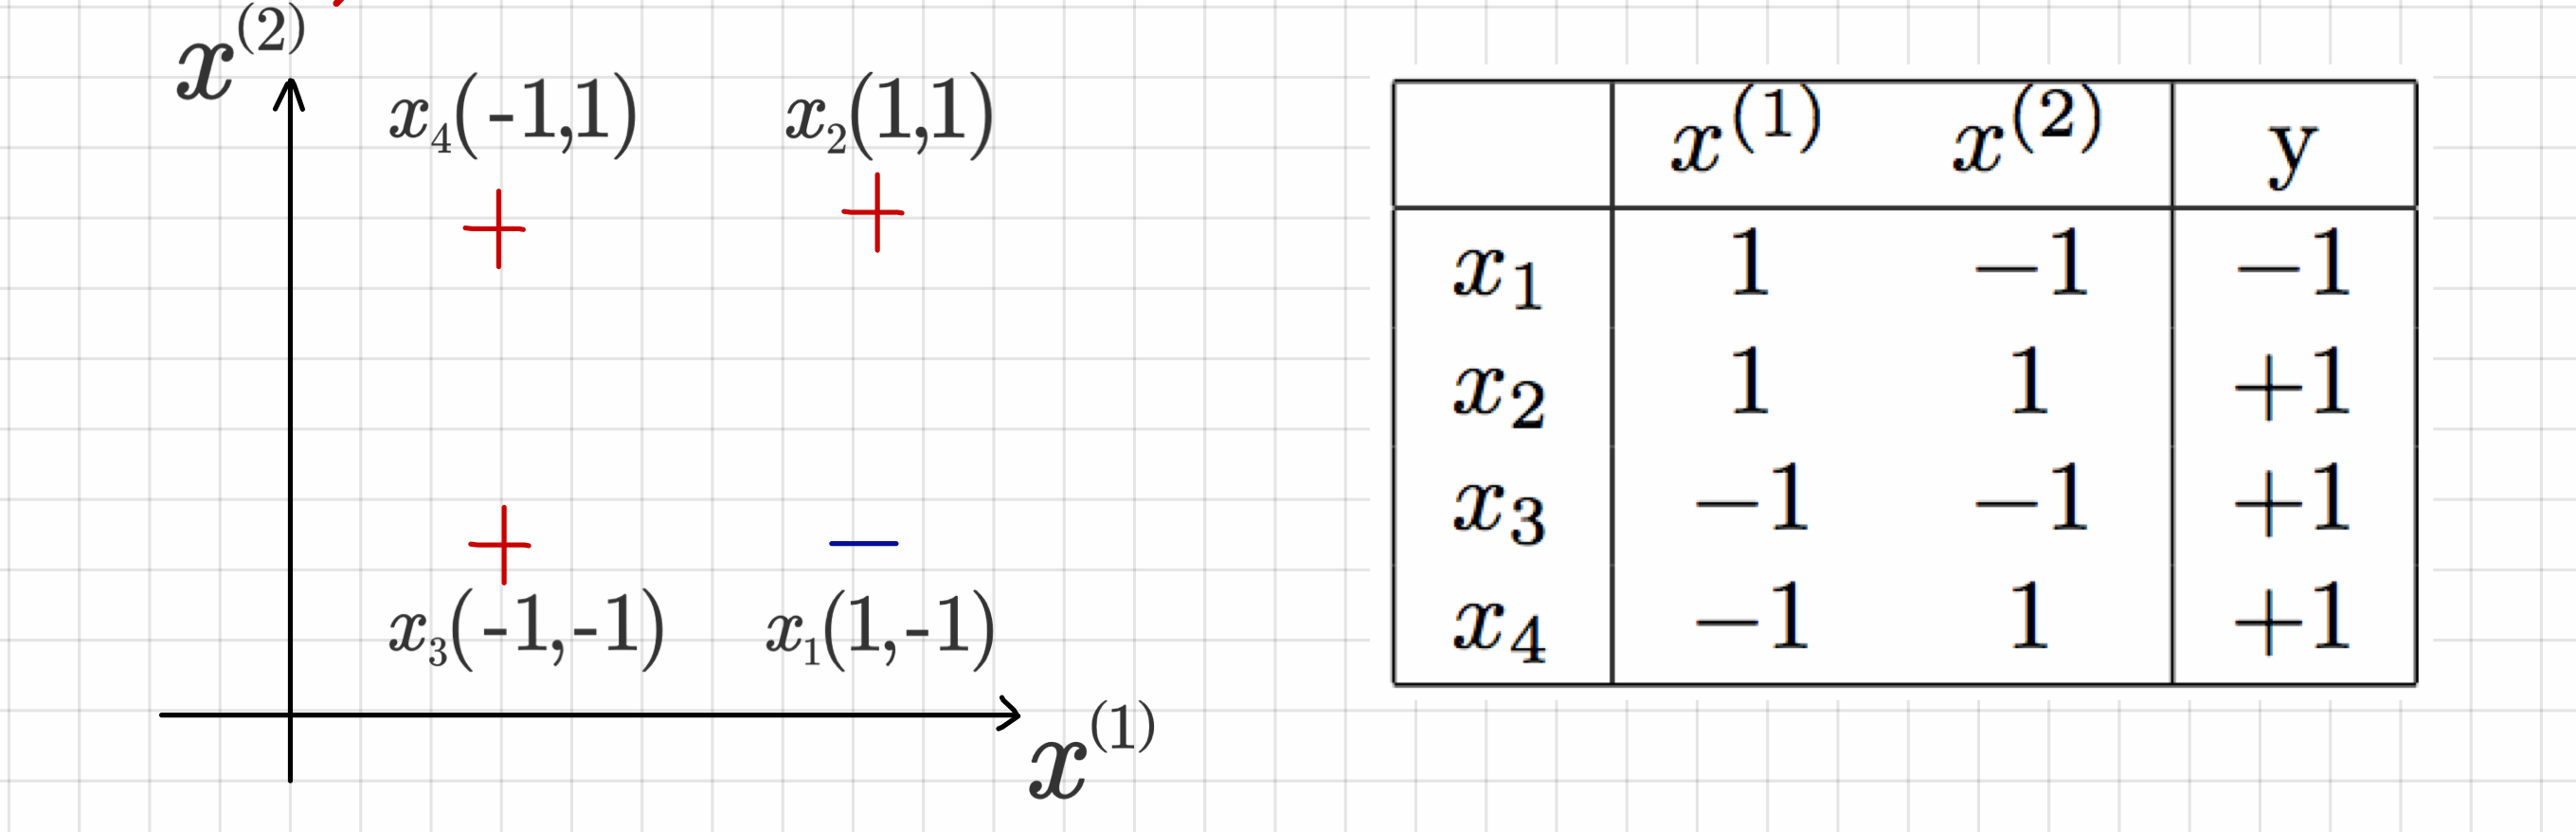
\includegraphics[width=3in] {SVM-figures/pic2.png}
\end{figure}
	
\begin{itemize}
	\item Given a set of samples with their category labels (denoted as $(\mathbf{x_{1}}, y_{1}), (\mathbf{x_{2}}, y_{2}), ...,  (\mathbf{x_{n}}, y_{n})$, $y_{i}\in \{-1, +1\}$, the goal of classification problem is to find an appropriate function $f(\mathbf{x})$ that can describe the dependency between $y_{i}$ and $\mathbf{x_{i}}$; thus, for a new sample $\mathbf{x'}$, we can infer its  category based on $f(\mathbf{x'})$. 
	\item A great variety of classification algorithms have been designed, including Fisher's linear discriminant, logistic regression, decision tree, neural network  and SVM. 
\end{itemize}

}

\frame{
	\frametitle{Linear classifier }
	
\begin{figure}
   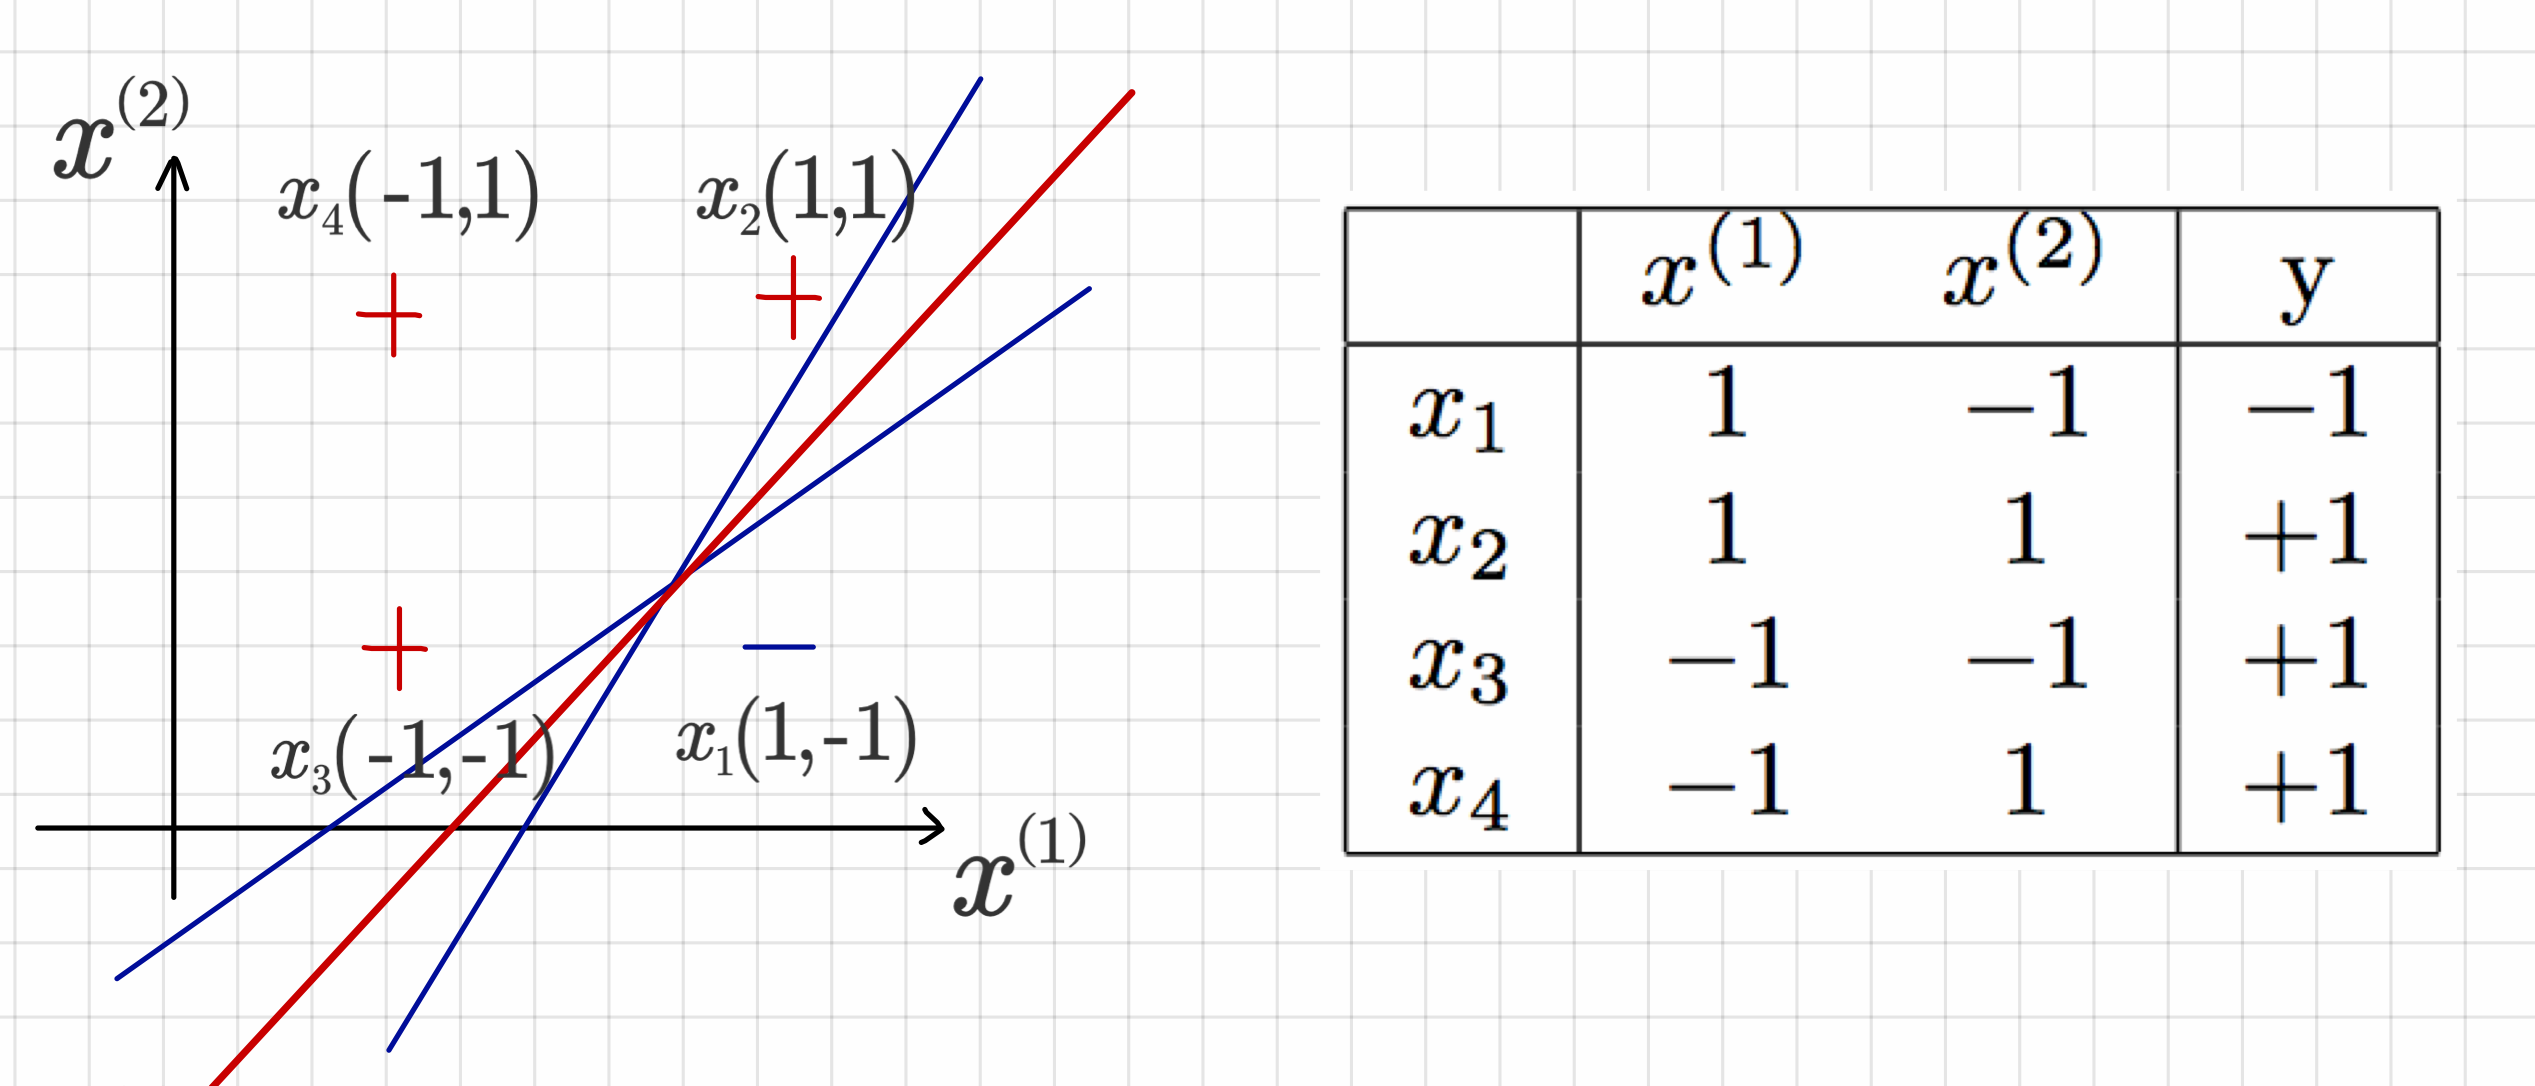
\includegraphics[width=3in] {SVM-figures/pic1.png}
\end{figure}

	\begin{itemize}
		\item Unlike decision tree, SVM adopts the classifier with the following type: 
			\begin{itemize}
				\item If $f(\mathbf{x})  > 0$ then $y = +1$; 
				\item If $f(\mathbf{x})  < 0$ then $y = -1$; 
			\end{itemize}
		\item Let's first restrict the  $f(\mathbf{x})$ to be linear, i.e. 
\[
	f(\mathbf{x})  = \mathbf{\omega}^{T}\mathbf{x} + b  
\]
		The hyperplane  $\mathbf{\omega}^{T}\mathbf{x} + b=0$ is denoted as separating hyperplane. 

	\end{itemize}
}

\frame{	


\begin{figure}
   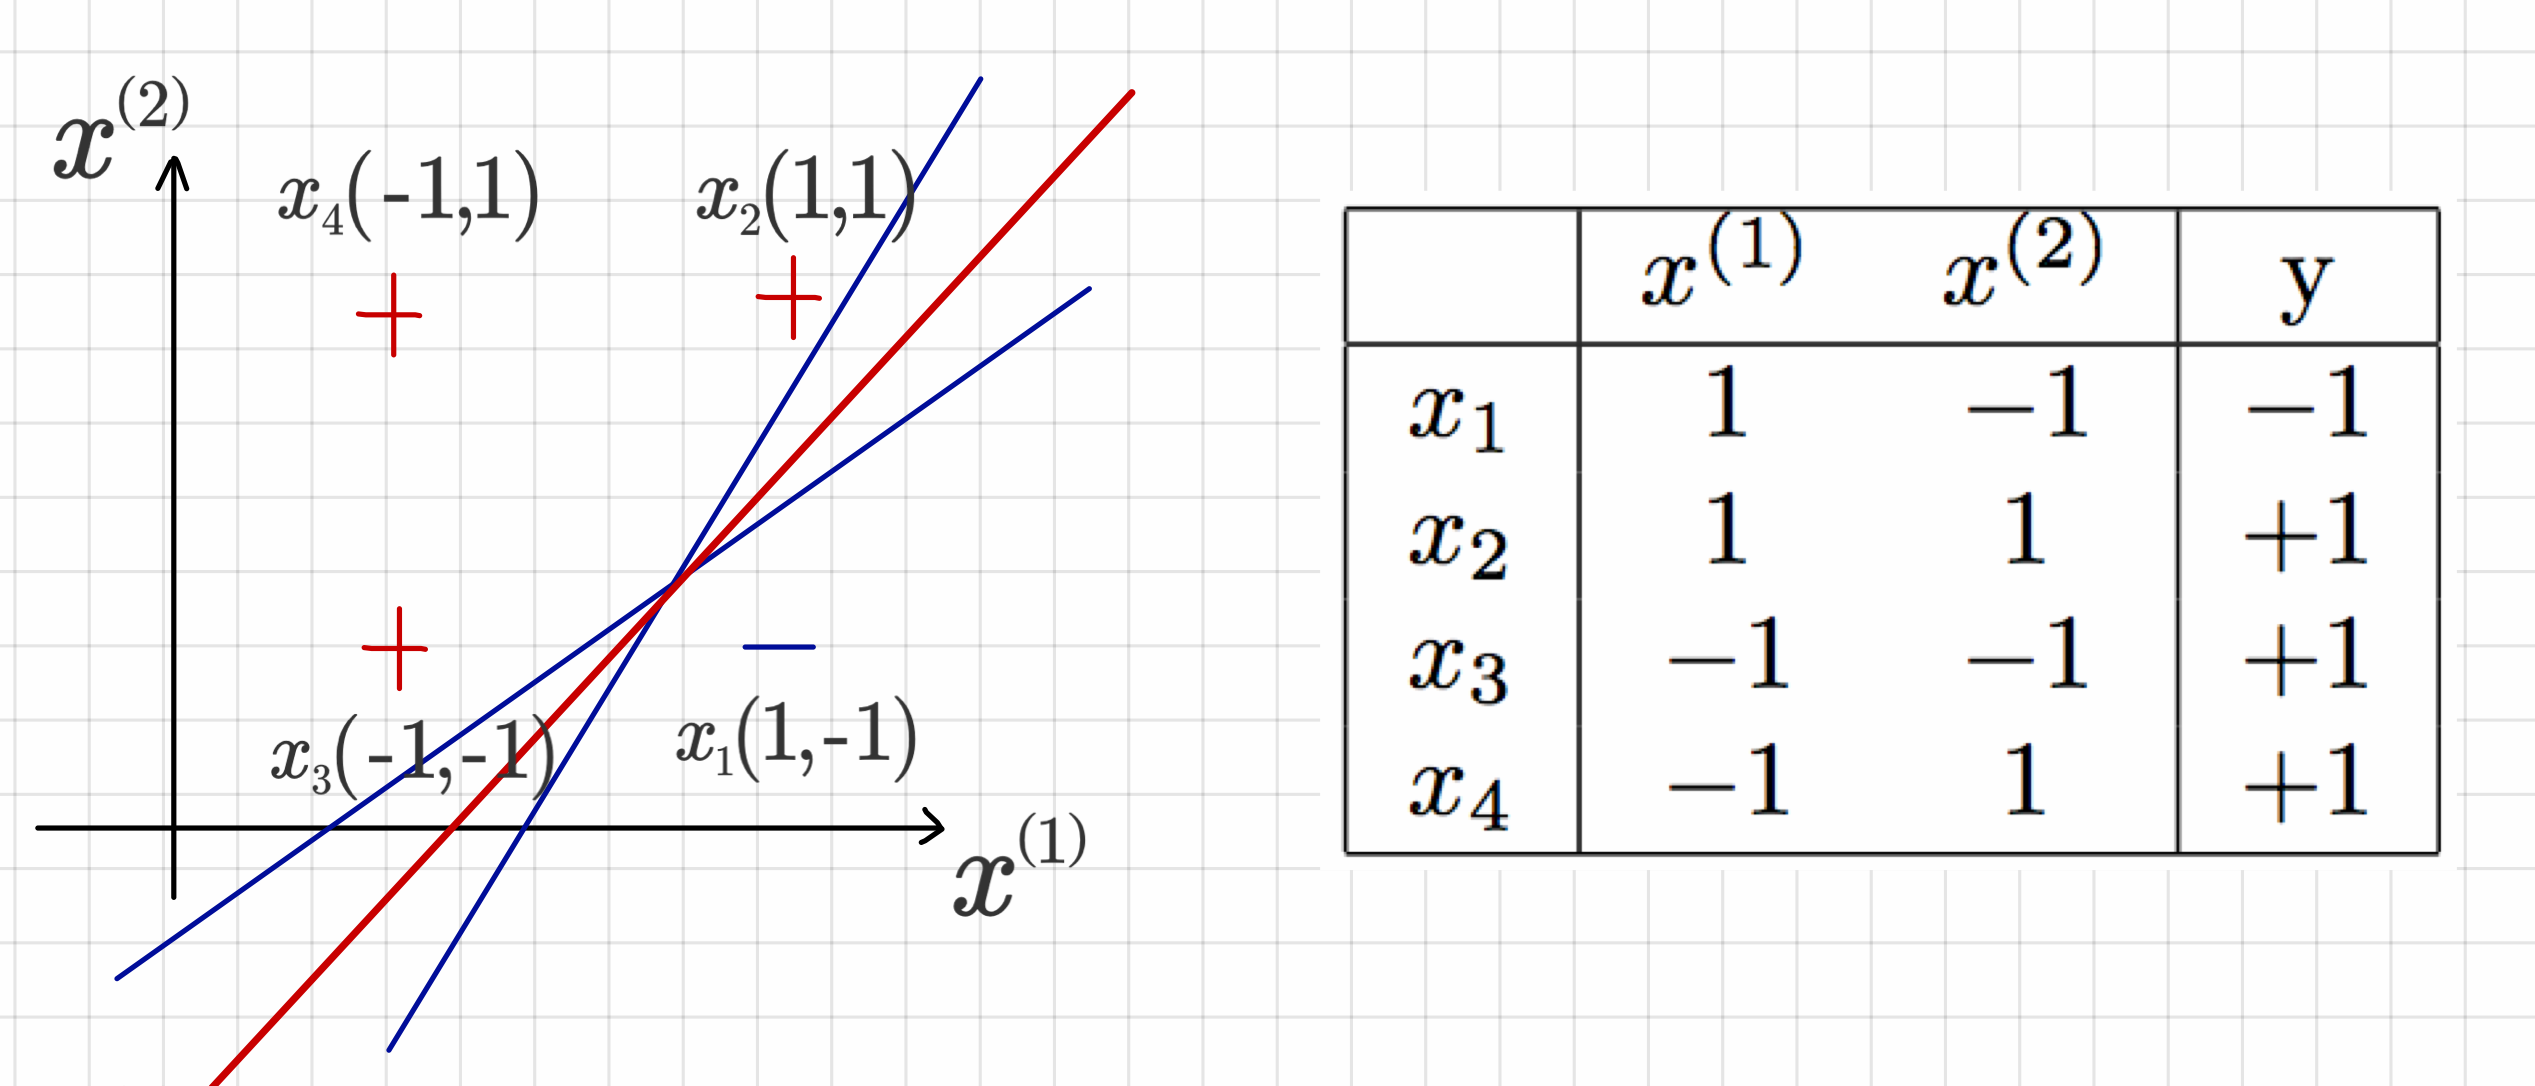
\includegraphics[width=3in] {SVM-figures/pic1.png}
\end{figure}
		\begin{itemize}
		\item The objective of training procedure is to find an appropriate setting of $\mathbf{\omega}$ and $b$ such that all samples in the training set can be correctly labelled using the classifier. We will consider the torlerance of several mislabelled samples later. 
	\end{itemize}
}


\frame{
	\frametitle{Maximum margin strategy} 

	\begin{itemize}
		\item There are always multiple settings of   $\mathbf{\omega}$ and $b$ that the corresponding classifier works perfectly on all samples. Which one should we use? 
		\item We prefer the one such that the margin between positive and negative samples is maximized: The wider the margin is, the larger the generality performance on new samples. Thus, we needs to solve the following optimization problem: 

\[
\begin{array}{rllllllll}
 \min_{{w},b} & \frac{2}{|| \mathbf{\omega} ||} &    \\
 s.t. & y_{i}(w\cdot x_{i}+b)-1\geqslant 0 & i=1,2,\cdots ,n \\
\end{array} \nonumber
\]
	
\item Note: 
	\begin{itemize}
		\item The restriction $f(\mathbf{x})  > 0$ for positive sample $x$ is implemented as $f(\mathbf{x})  = 1$.  
		\item The distance for any point $x$ to the hyperplane $\mathbf{\omega}^{T}\mathbf{x} + b=0$ is $\frac{| \mathbf{\omega}^{T}\mathbf{x} + b |}{|| \mathbf{\omega} ||}$. Thus, the margin is: $\frac{2}{|| \mathbf{\omega} ||}$.
	\end{itemize}

\end{itemize}

}


\frame{
	\frametitle{An equivalent form with quadratic objective function} 

	\begin{itemize}
		\item An equivalent form  is: 
\[
\begin{array}{rllllllll}
 \min_{{w},b} & \frac{1}{2}\left \| {w} \right \|^{^{2}} &    \\
 s.t. & y_{i}(w\cdot x_{i}+b)-1\geqslant 0 & i=1,2,\cdots ,n \\
\end{array} \nonumber
\]
	
		\item Question: how to solve this  optimization problem subject to inequality constraints? 
		\item Of course we solve the problem (called primal problem hereafter) directly using convex quadratic programming  techniques; however, consider its dual problem will bring great benefits.  
		\item Let's review the conditions of the optimal solution first. 

\end{itemize}

}


\frame{
\frametitle{Lagrangian dual explanation of maximum margin problem }
\begin{itemize}
\item Primal problem: 
\[
\begin{array}{rrrrrrrrl}
\min_{w,b} & \frac{1}{2}\left \| w \right \|^{^{2}} & & &\\
s.t. &y_{i}(w^{T}x_{i}+b) &\geq &1, & i\in {\{1,..., n\}}
\end{array} \nonumber
\]
\item 
Lagrangian: 
\begin{center}
$L(w,b,\alpha )=\frac{1}{2}\left \| w \right \|^{2}- \sum_{i=1}^{n}\alpha _{i}y_{i}(w\cdot x_{i}+b)+\sum_{i=1}^{n}\alpha _{i}$ 
\end{center}
% \begin{itemize}
%  \item $\lambda_i$ are called Lagrangian multipliers; 
%  \item objective is augmented with weighted sum of constraint functions; 
% \end{itemize}
\item Notice that \textcolor{red} {\textcolor{red}{\bf Lagrangian is a lower bound of the primal objective function}}, i.e. ${ \frac{1}{2}\left \| w \right \|^{^{2}}} \geq L({w, b,\alpha})$, when $\mathbf{\alpha \geq 0}$ and $\mathbf{w,b}$ is feasible.

 \item Furthermore we have  
\[
{ \frac{1}{2}\left \| w \right \|^{^{2}}} \geq L({w,b,\alpha}) \geq \inf_{{{w,b}} } L({w,b}, {\alpha} )  
\]
when ${\alpha \geq 0}$ and ${w,b}$ is feasible.
 
 \item Denote \textcolor{red}{\bf Lagrangian dual} $g({\alpha} ) = \inf_{{w,b} } L( {w,b}, {\alpha} )$. The above inequality can be rewritten as:
 \[
 { \frac{1}{2}\left \| w \right \|^{^{2}}} \geq L({w,b, \alpha}) \geq g({\alpha} ) 
 \]
 
% \item We further have the following inequality: 
% \[
% \mathbf{c^T x} \geq L(\mathbf{x, \lambda}) \geq \max_{\mathbf{\lambda}} g(\mathbf{\lambda} )
% \]
%  \item 
% In other words, $\max_{\mathbf{\lambda}} g(\mathbf{\lambda} )$ serves as a tight lower bound of $\mathbf{c^T x}$ for any feasible solution $\mathbf{x}$ (if $\mathbf{\lambda \leq 0} $).
 \end{itemize}
} 
 
% 
% 
% 
% Thus $p^* \geq \min_{\hat{x}} L( \hat{x}, \lambda)$ if $\lambda \geq 0 $. 
\frame{
\frametitle{Lagrangian dual function} 
\begin{itemize}
\item 
What is the Lagrangian dual $g({ \alpha})$? 
\begin{eqnarray}
 g({\alpha}) &= & \inf_{{w,b}} L( {w,b, \alpha} ) \nonumber
\end{eqnarray}
\item To calculate the inferior bound  of $L( {w,b},\alpha )$, we set its derivates  to be 0, i.e.,  
$$\frac{\partial L(w,b,\alpha)}{\partial w}=w-\sum_{i=1}^{n}\alpha_{i}y_{i}x_{i}=0$$
$$\frac{\partial L(w,b,\alpha)}{\partial b}=\sum_{i=1}^{n}\alpha_{i}y_{i}=0$$
and obtain  Lagrangian dual function: $$g(\alpha) = -\frac{1}{2}\sum_{i=1}^{n}\sum_{j=1}^{n}\alpha_{i}\alpha_{j}y_{i}y_{j}(x_{i}^{T} x_{j})+\sum_{i=1}^{n}\alpha_{i}$$
%subject to the constraint $$\sum_{i=1}^{N}\alpha_{i}y_{i}=0$$. 
\item Thus $ g(\mathbf{\alpha})$ is a lower bound of $\frac{1}{2}\left \| w \right \|^{^{2}}$ when  $\sum_{i=1}^{n}\alpha_{i}y_{i}=0$ and ${\alpha \geq 0}$. 

\end{itemize} 
} 

%\frame{
%\frametitle{Lagrangian dual  function} 
%\begin{itemize}
%\item 
%Lagrangian dual function: $$g(\alpha) = -\frac{1}{2}\sum_{i=1}^{n}\sum_{j=1}^{n}\alpha_{i}\alpha_{j}y_{i}y_{j}(x_{i}^{T} x_{j})+\sum_{i=1}^{n}\alpha_{i}$$
%%subject to the constraint $$\sum_{i=1}^{N}\alpha_{i}y_{i}=0$$. 
%\item Thus $ g(\mathbf{\alpha})$ is a lower bound of $\frac{1}{2}\left \| w \right \|^{^{2}}$ when  $\sum_{i=1}^{n}\alpha_{i}y_{i}=0$ and ${\alpha \geq 0}$. 
%%The difference $f(\mathbf{x}) -  g(\mathbf{\lambda})$ is called \textcolor{red}{\bf duality gap}. 
%%\item Note $g(\mathbf{\alpha})$ is always concave even if the constraints are not convex. 
%\end{itemize} 
%} 
\frame{
\frametitle{Lagrangian dual problem}  
\begin{itemize}
\item Now let's try to find  \textcolor{red}{\bf the tightest  lower bound} of $\frac{1}{2}\left \| w \right \|^{^{2}}$, which can be calculated by solving the following Lagrangian dual problem: 
\[
\begin{array}{rrrrrrrrl}
 \max & -\frac{1}{2}\sum_{i=1}^{n}\sum_{j=1}^{n}\alpha_{i}\alpha_{j}y_{i}y_{j}(x_{i}^{T} x_{j})+\sum_{i=1}^{n}\alpha_{i} & &\\
 s.t. & \sum_{i=1}^{n}\alpha_{i}y_{i} &= &0  \\ 
      & {\alpha}&\geq&{0 }
\end{array} \nonumber
\]

\item The dual problem has an identical optimal objective function value to the primal problem as the Slater's conditions hold. 
\item One advantage of the dual problem is that $x_i$ and $x_i$ appears in the form of inner product $x_{i}^{T} x_{j}$; thus, we can simply define a kernel function $k(x_i, x_j) = \phi(x_{i})^{T} \phi(x_{j})$ without knowing the details of map $\phi(.)$. 

\end{itemize} 
%$g(\lambda) = \min_{\hat{x}} L( \hat{x}, \lambda)$.
}

\end{document}

%\frame{
%\frametitle{An example } 
%\begin{itemize}
% \item 
%Primal problem: 
%\[
%\begin{array}{rrrrrrrrl}
% \min & x & &   \\
% s.t. & x & \geq& 2 \\ 
%      & x & \geq& 0 
%\end{array} \nonumber
%\]
%\item 
%Lagrangian: 
%\begin{center}
%$L(x,y) = x - y*(x-2 ) = 2y + x*(1-y)$ 
%\end{center}
%\item When $y\geq 0$ and $x\geq 2$,  $L(x, y)$ is a lower bound of $x$. 
%\item Lagrangian dual function: 
%\begin{center}
%$g(y) = \inf_x L(x,y) =  \begin{cases} 2y & \text{ if } x\geq 0 \text{ and } (1-y)\geq 0  \\ 
%                                                          -\infty & \text{ otherwise } 
%                                     \end{cases} $
%\end{center}
%
%
%\item 
%Dual problem: 
%\[
%\begin{array}{rrrrrrrrl}
% \max & 2y    \\
% s.t. & y  \leq 1 \\ 
%      & y  \geq 0 
%\end{array} \nonumber
%\]
%\end{itemize}
%}


%\frame{
%\frametitle{Lagrangian connecting primal and dual cont'd } 
%\begin{figure}
% \includegraphics[width=2.5in,angle=-90] {L9-Lagrangian-duality-example2-2.eps}
%\end{figure}
%\begin{itemize}
%\item 
%Observation: {\sc Primal} objective function $x$ intersects {\sc Dual} objective function $y$ at the saddle point of Lagrangian.
%\end{itemize}
%
%(See extra slides.)
%} 



\frame{ 
\frametitle{Two explanations of dual variables $\mathbf{y}$: L. Kantorovich vs. T. Koopmans } 

\begin{enumerate}
\item 
Price interpretation: constrained optimization plays an important role in economics. Dual variables are also called as \textcolor{red}{\bf shadow price} (by T. Koopmans), i.e.  the instantaneous change in the optimization objective function when constraints are relaxed, or \textcolor{red}{\bf marginal cost} when strengthening constraints. 
\ \\

\item 
\textcolor{red}{\bf Lagrangian multiplier}: the effect of constraints on the objective function (by L. Kantorovich). For example, when $b_{i}$ increase to $b_{i}+\Delta b_{i}$, how much the objective function value will change. In fact, we have $\frac{\partial L(\mathbf{x}, \mathbf{\lambda})}{\partial b_{i}} = \lambda_{i}$. 
\end{enumerate}

} 
%\frame{
%	\frametitle{Shadow price} 
%	
%	\begin{figure}
%		
\includegraphics[width=3in]{L9-shadowprice.eps}
%	\end{figure}	
%}


\frame{
\frametitle{Explanation of dual variables $y$: using {\sc Diet} as an example} 
\begin{itemize} 
 \item Optimal solution to primal problem with $b_1=2000, b_2 = 55, b_3=800$:  \\
\qquad $\mathbf{x}=(14.24, 2.70, 0, 0)$, \\
\qquad $\mathbf{c^Tx}=67.096$.
 \item Optimal solution to dual problem: \\
\qquad $\mathbf{y}=(0.0269, 0, 0.0164)$, \\
\qquad $\mathbf{y^Tb}=67.096$.  
 \item Let's make a slight change on $\mathbf{b}$, and watch the effect on $\max \mathbf{c^Tx}$.
 \begin{enumerate}
\item $b_1= 2001$: $\max \mathbf{c^Tx}=67.123$ \ \ (Note that $\mathbf{y_1}=0.0269 = 67.123 - 67.096$)
\item $b_2=\quad 56$: $\max \mathbf{c^Tx}=67.096$ \ (Note that $\mathbf{y_2}=0  = 67.096 - 67.096$)
\item $b_3=\ \ 801$: $\max \mathbf{c^Tx}=67.112$ (Note that $\mathbf{y_3}=0.0164  = 67.112 - 67.096$)
\end{enumerate}
\end{itemize}
(See extra slides)
}


\frame{
\begin{block}{}
	Weak duality, strong duality, and Slater conditions
\end{block}
}

\frame{
	\frametitle{Weak duality and strong duality}
	
\begin{figure}
   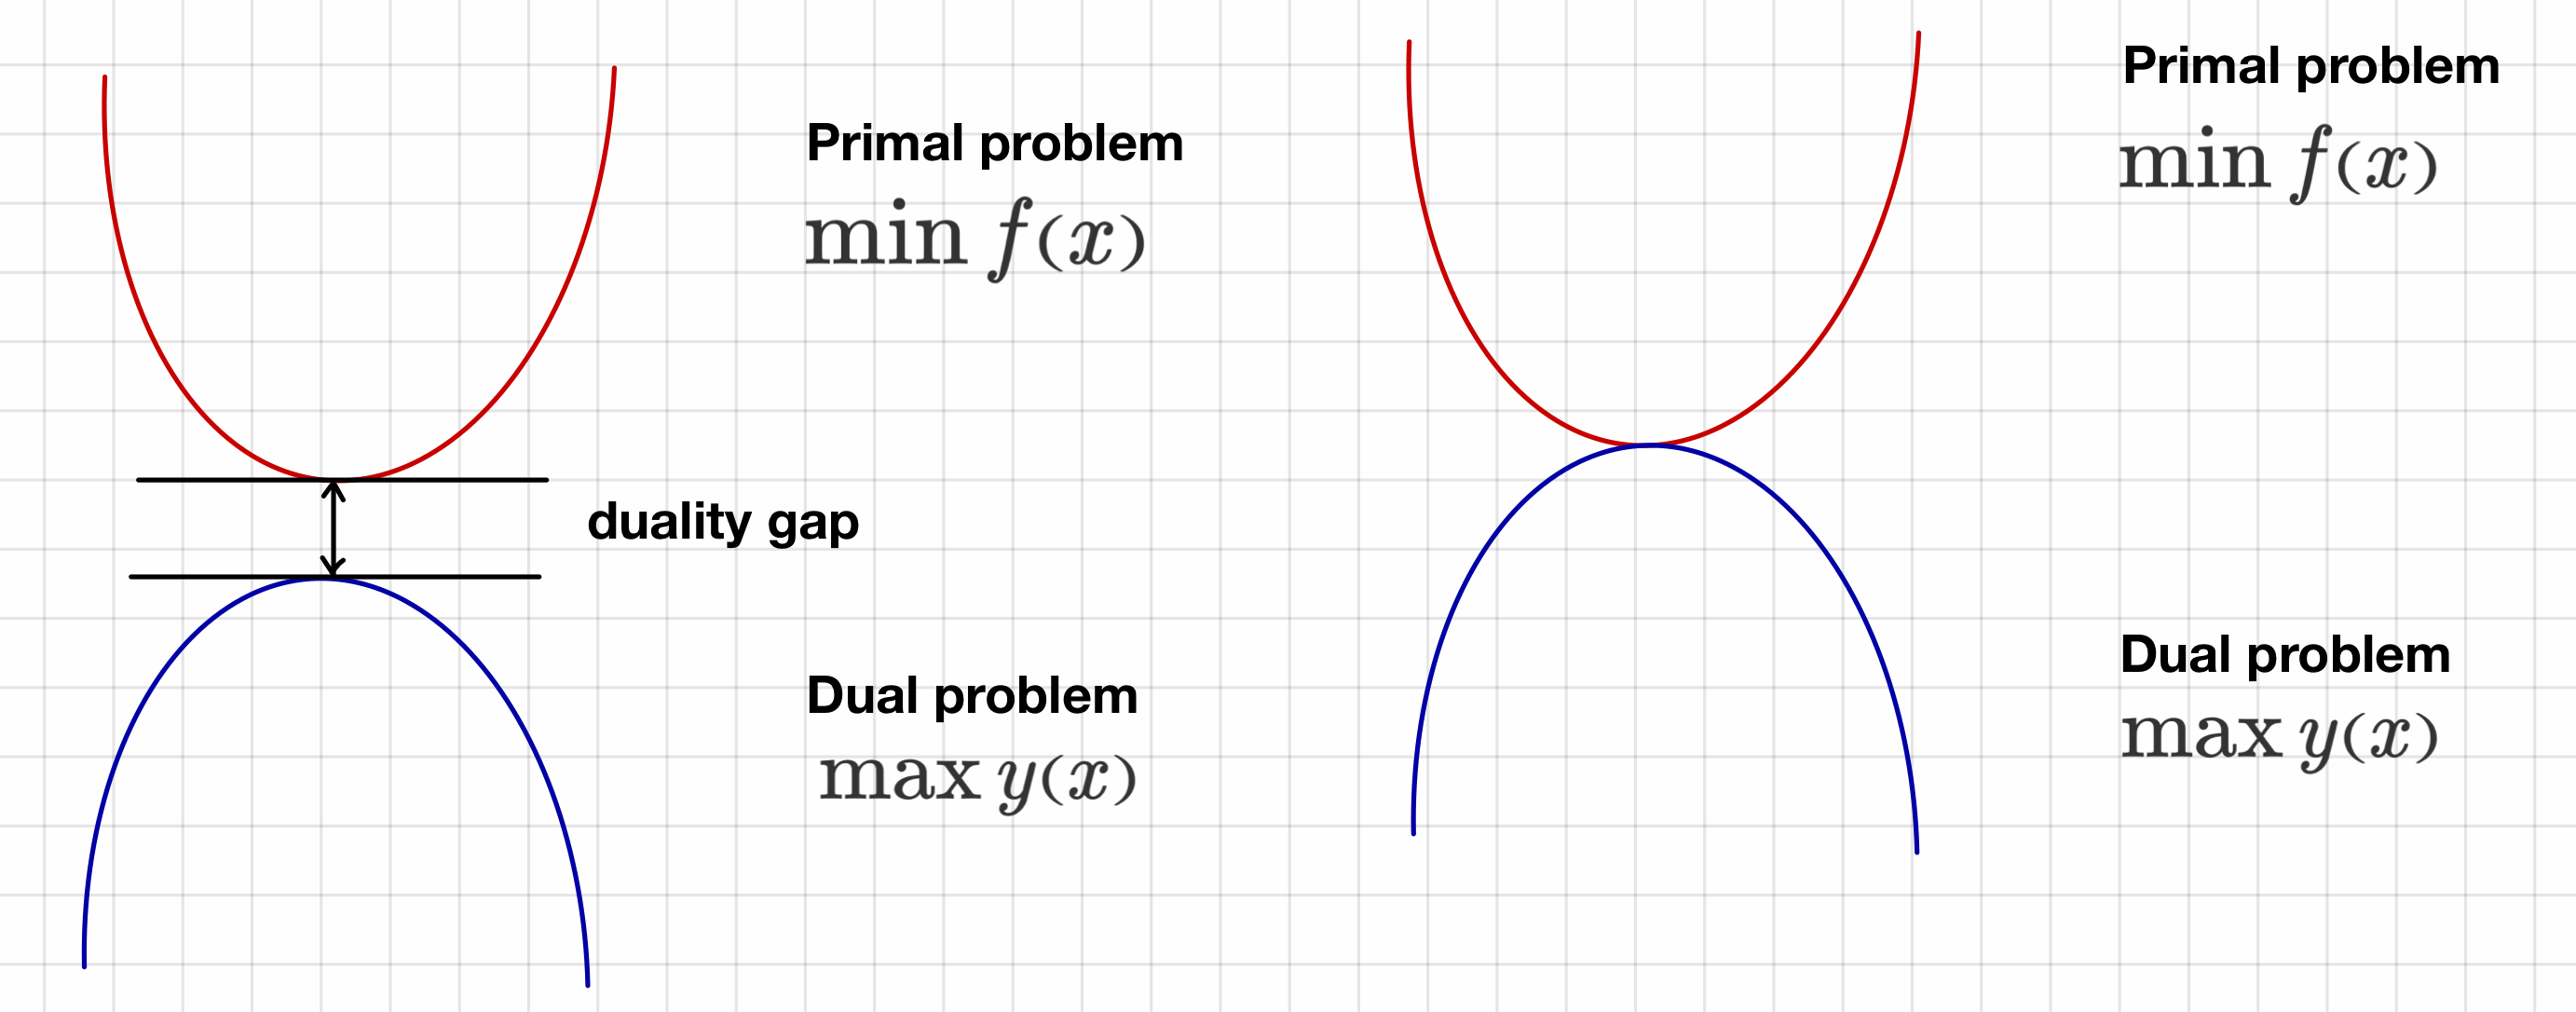
\includegraphics[width=3in] {SVM-figures/pic6.png}
\end{figure}

	\begin{itemize}
		\item Sometimes the optimal solution of the primal problem doesn't has identical value to that of the dual problem. The difference between them is denoted as duality gap. This case is denoted as weak duality. The opposite case is denoted as strong duality. 
		\item Conditions under which strong duality holds are denoted as \textcolor{red}{\bf constraint qualifications}.
	\end{itemize}

}

\frame{
	\frametitle{Slater's conditions for strong duality}
	
	\begin{itemize}
		\item The best known sufficient condition of strong duality is: 
			\begin{itemize}
				\item Primal problem is convex programming, i.e., 
\[
\begin{array}{rrrrrrrrl}
 \min & f( \mathbf{x})  &   & \\
 s.t. & g_i( \mathbf{x})  &\textcolor{red}{\bf \leq} & 0 & i=1,2,...m\\
       
      & \mathbf{A x}   &\textcolor{red}{\bf =} & \mathbf{b} & 
\end{array} \nonumber
\]
where $f(x)$ and $g_{i}(x)$ are convex. 			
				\item Slater's condition holds, i,e. there exists some strictly feasible point $x \in relint(\mathcal{D})$ such that 
\[ 
\mathbf{A x = b}
\] and 
\[
g_{i}(\mathbf{b}) \textcolor{red}{\bf <} 0, i=1, 2, ..., m
\]  
Here $\mathcal{D}$ represents the feasible domain of the primal problem, and $relint(\mathcal{D})$  denotes the relative interior of  $\mathcal{D}$. 				 
			\end{itemize}

	\end{itemize}

	
}


\frame{
	\frametitle{Slater's conditions for strong duality (cont'd)}
	
	\begin{itemize}
		\item The Slater's conditions are trivial if the constraints of the primal problem are affine, i.e., Consider the following convex programming  problem:  
\[
\begin{array}{rrrrrrrrl}
 \min & f( \mathbf{x})  &   & \\
 s.t. & g_i( \mathbf{x})  &\textcolor{red}{\bf \leq} & 0 & i=1,2,...m\\
       
      & \mathbf{A x}   &\textcolor{red}{\bf =} & \mathbf{b} & 
\end{array} \nonumber
\]
where $f(x)$ and $g_{i}(x)$ are convex. 			
				\item Slater's condition: If $g_{i}(x)$ are affine, the inequalities are no longer required to be strict and thus reduce to the original form, i.e. there exists some strictly feasible point $x \in relint(\mathcal{D})$ such that		
\[ 
\mathbf{A x = b}
\] and 
\[
g_{i}(\mathbf{b}) \textcolor{red}{\bf \leq} 0, i=1, 2, ..., m
\]  		 
	\end{itemize}
} 

\frame{
	\frametitle{Strong duality in SVM} 
	
	\begin{figure}
   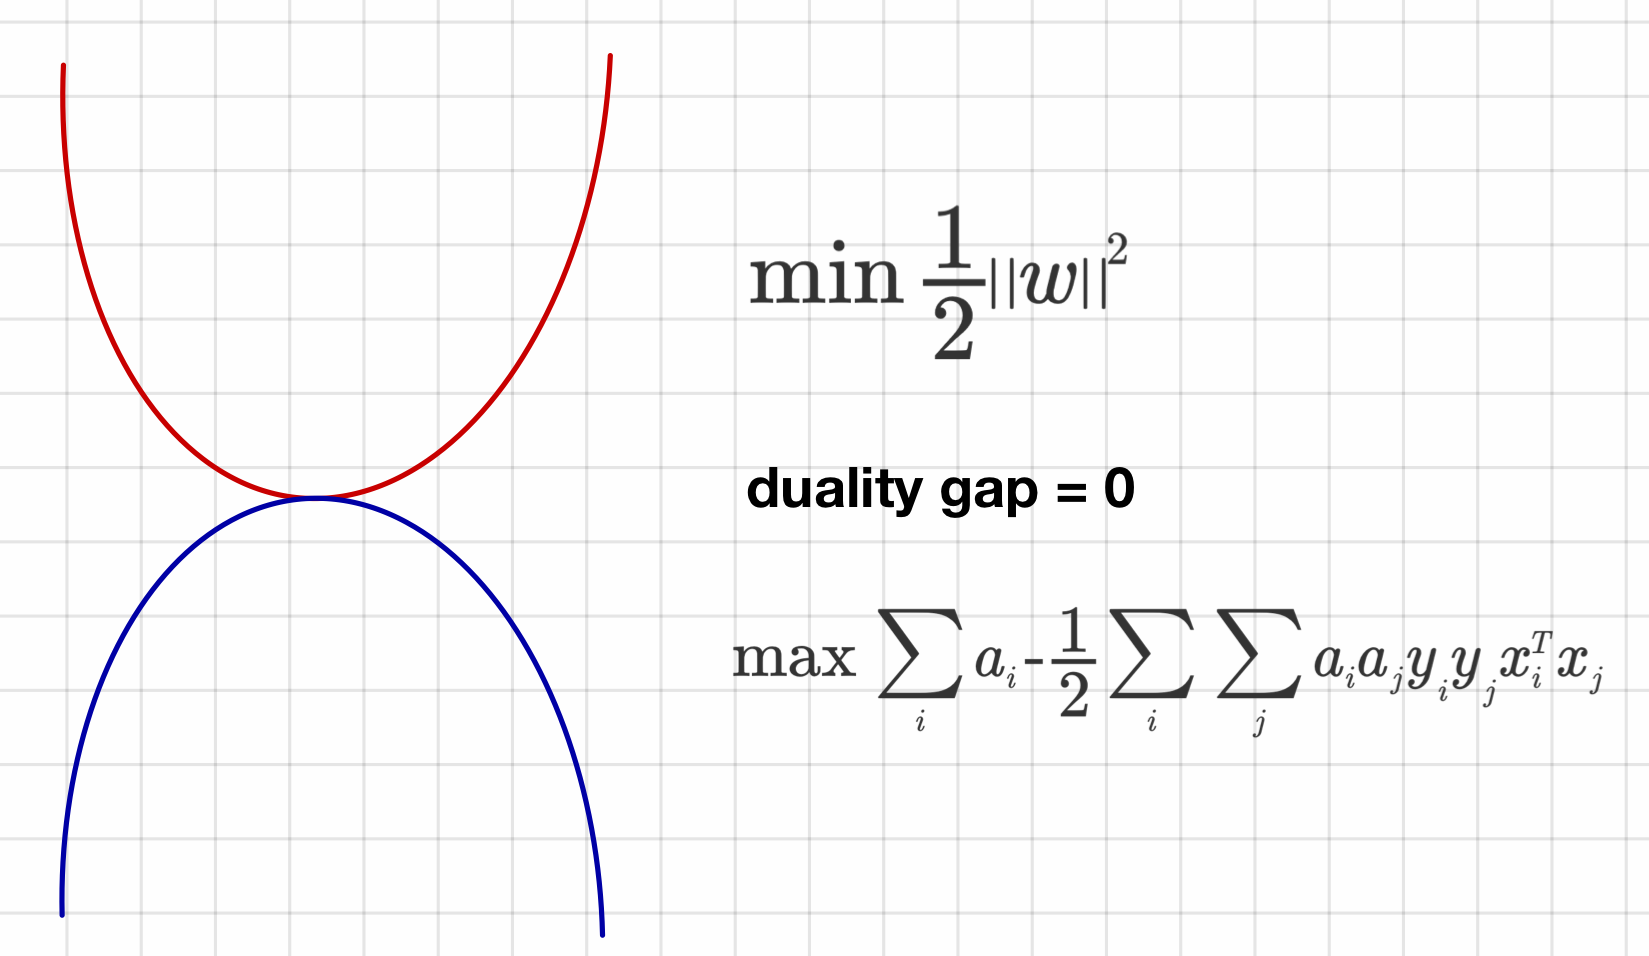
\includegraphics[width=3in] {SVM-figures/pic5.png}
\end{figure}
	\begin{itemize}

		\item For the maximum margin problem, its dual problem has the identical optimal objective function value.  		 
	\end{itemize}
}





\frame{
\begin{block}{}
Kernel method to overcome linear insperability
\end{block}
}

\frame{
	\frametitle{Linearly inseperable  } 
	
\begin{figure}
   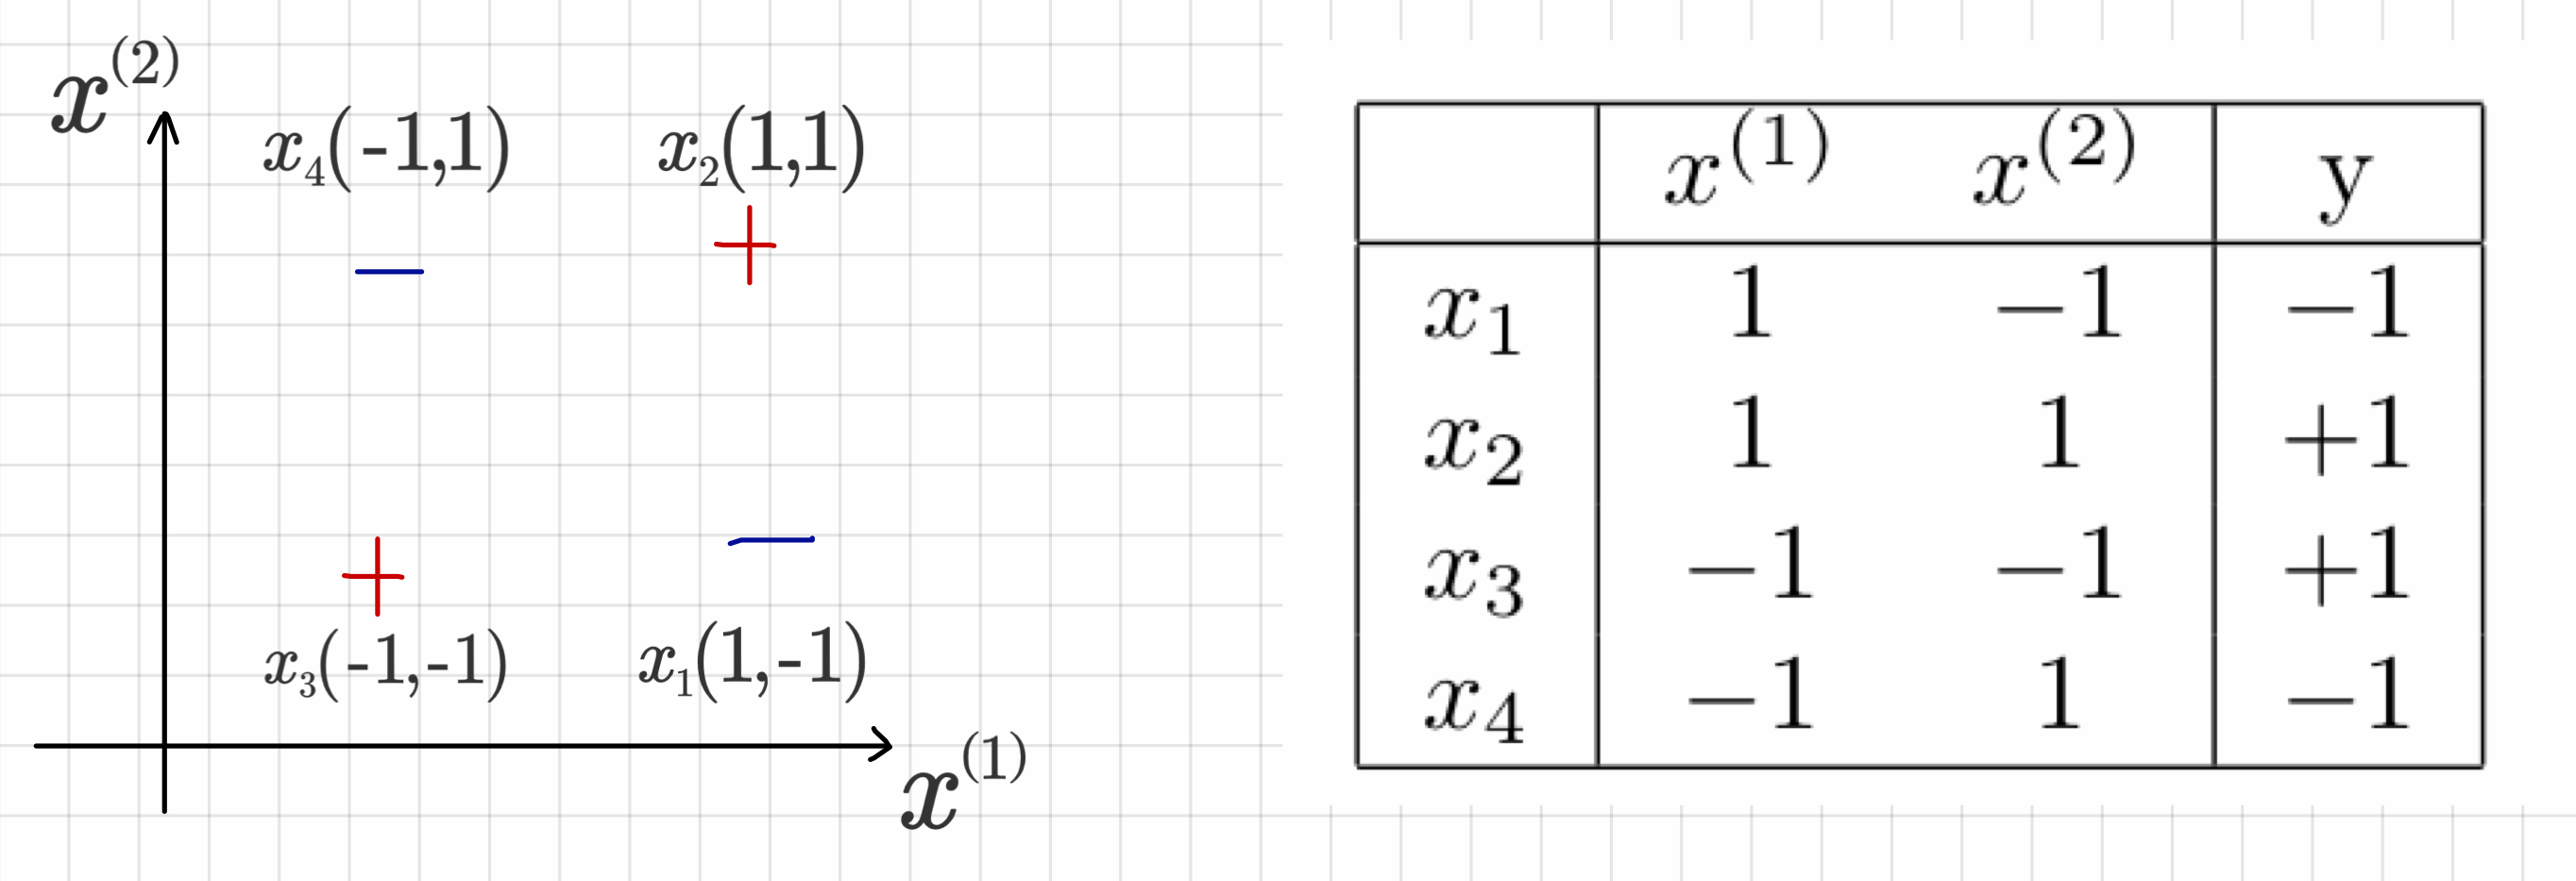
\includegraphics[width=3in] {SVM-figures/pic3.png}
\end{figure}

	
	\begin{itemize}
		\item Some samples are linearly insuperable. How should we do? 
		\item Kernel method: If the samples are linearly inseperable in the original input space, let's map them into a higher-dimensional space (called feature space) and make them linearly separable in that space. In other words, nonlinearity was introduced into the original input space through using the map. 
	\end{itemize}
}

\frame{
	\frametitle{An example: {\sc XOR} problem}


\begin{figure}
   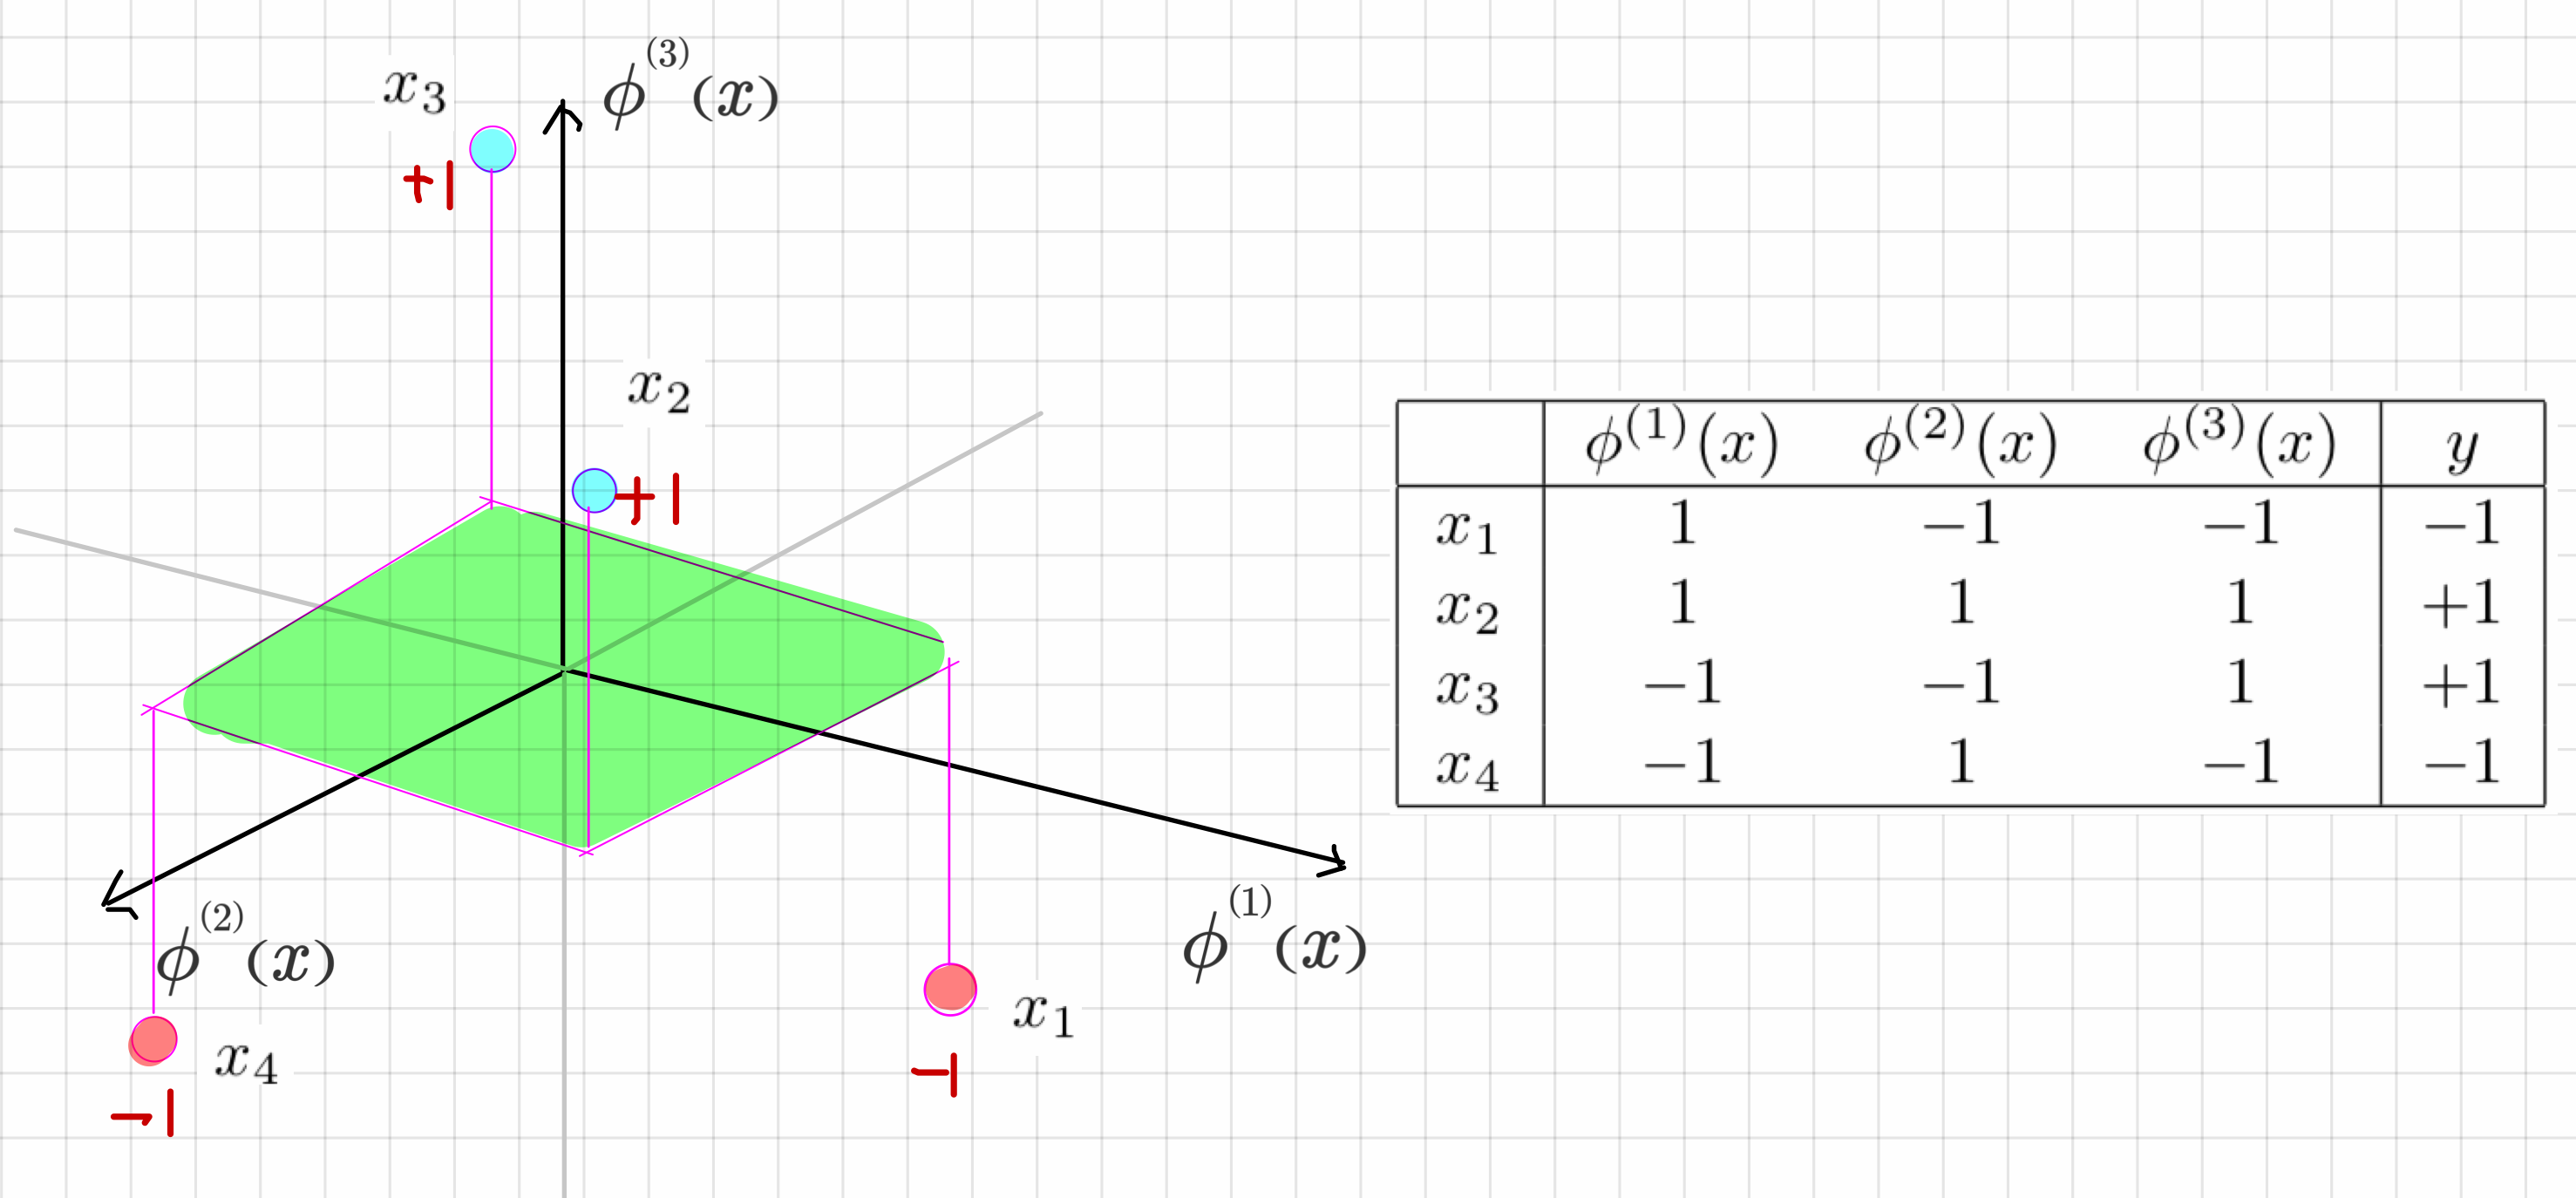
\includegraphics[width=3in] {SVM-figures/pic7.png}
\end{figure}
	
	\begin{itemize}
		\item Let's define a map: $\phi: \mathbb{R}^{2} \rightarrow \mathbb{R}^{3}$ as below: 
		
		\[
			[ x^{(1)}, x^{(2)} ] \rightarrow \Phi(  [ x^{(1)}, x^{(2)} ]  ) = [ x^{(1)}, x^{(2)}, x^{(1)}x^{(2)} ] 
		\]
		\item These samples are linearly seperable after mapping into $\mathbb{R}^{3}$ using $	\Phi(   x^{(1)}, x^{(2)} )$	

	\end{itemize}
}

\frame{
	\frametitle{Replace the inner product in the optimization problem for SVM}
	
	\begin{itemize}
		\item Remember that in the optimization problem for SVM, the objective function contains inner product $\mathbf{x}^{T}\mathbf{x}$:
\[
\begin{array}{rrrrrrrrl}
 \max & -\frac{1}{2}\sum_{i=1}^{N}\sum_{j=1}^{N}\alpha_{i}\alpha_{j}y_{i}y_{j}(x_{i}^{T} x_{j})+\sum_{i=1}^{N}\alpha_{i} \\
 s.t. & \sum_{i=1}^{N}\alpha_{i}y_{i}=0  \\ 
      & \mathbf{\alpha}\geq\mathbf{0 }
\end{array} \nonumber
\]
		
		
		\item After mapping $\mathbf{x}$ into  $\mathbf{\Phi(x)}$, the inner product $\mathbf{x}^{T}\mathbf{x}$ changes into $\mathbf{\Phi(x)}^{T}\mathbf{\Phi(x)}$, and the optimization problem changes accordingly: 
		
\[
\begin{array}{rrrrrrrrl}
 \max & -\frac{1}{2}\sum_{i=1}^{N}\sum_{j=1}^{N}\alpha_{i}\alpha_{j}y_{i}y_{j}(\Phi(x_{i})^{T} \Phi(x_{j}))+\sum_{i=1}^{N}\alpha_{i} \\
 s.t. & \sum_{i=1}^{N}\alpha_{i}y_{i}=0  \\ 
      & \mathbf{\alpha}\geq\mathbf{0 }
\end{array} \nonumber
\]
		
		Note we simply  replace this inner product with $\mathbf{\Phi(x)}^{T}\mathbf{\Phi(x)}$ \textcolor{red}{\bf without even knowing the map $\mathbf{\Phi(x)}$}. 
		
		\item In other words, we define a kernel function 
\[
k( \mathbf{x}_{i}, \mathbf{x}_{j} ) = < \mathbf{\Phi(x_{i})},  \mathbf{\Phi(x_{j})}>_{\mathcal{H}_{k}}
\]
Here $\mathcal{H}_{k}$ represents the reproducing kernel Hilbert space with respect to $k(.,.)$.	
	\end{itemize}
}

\frame{
	\frametitle{The seperating hyperplane}
	
	\begin{itemize}
		\item Remember that in the optimization problem for SVM, the seperating hyperplane is: 
	
\[
	f(\mathbf{x}) = \mathbf{\omega}^{T}\mathbf{x} + b = \sum_{i,j} \alpha_{i} y_{i}\mathbf{x}_{i}^{T}\mathbf{x}  = 0 
\]
		
		
		\item After mapping $\mathbf{x}$ into  $\mathbf{\Phi(x)}$,  the sporting hyperplane changes into: 
\[
	f(\mathbf{x}) = \mathbf{\omega}^{T}\mathbf{\Phi(x)}+ b = \sum_{i,j} \alpha_{i} y_{i}\mathbf{\Phi(x)}_{i}^{T}\mathbf{\Phi(x)}  = 0 
\]
		 \item Note that $\mathbf{\Phi(x)}_{i}^{T}\mathbf{\Phi(x)} = k(\mathbf{\Phi(x)}_{i}, \mathbf{\Phi(x)})$.
	\end{itemize}
 
}


\frame{
	\begin{block}{}
		Deriving  kernel function from map
 	\end{block}
}

\frame{
	\frametitle{Example 1}  

	\begin{itemize}
		\item Consider the map $\Phi: \mathbb{R}^{2} \rightarrow \mathbb{R}^{4}$:  
		\[
			[ x^{(1)}, x^{(2)} ] \rightarrow \Phi(  [ x^{(1)}, x^{(2)} ]  ) = [ x^{(1)2}, x^{(2)2}, x^{(1)}x^{(2)},  x^{(1)}x^{(2)}] 
		\]
		
		\item The corresponding kernel function is: 
		
\[
	k( \mathbf{x}, \mathbf{z} ) = x^{(1)2} z^{(1)2} + x^{(2)2}z^{(2)2} + 2x^{(1)}x^{(2)}z^{(1)}z^{(2)} = <\mathbf{x}, \mathbf{z} >^{2}_{\mathbb{R}^{2}}
\]		
	\end{itemize}

}

\frame{
	\frametitle{Example 2}  

	\begin{itemize}
		\item Consider the map $\Phi: \mathbb{R}^{3} \rightarrow \mathbb{R}^{13}$:  
		\[
			[ x^{(1)}, x^{(2)}, x^{(3)} ] \rightarrow \Phi(  [ x^{(1)}, x^{(2)}, x^{(3)} ]  ) = [ x^{(1)2}, x^{(1)}x^{(2)}, ...,  x^{(3)2},  \sqrt{2c} x^{(1)}, ..., c] 
		\]
		
		\item The corresponding kernel function is: 
		
\[
	k( \mathbf{x}, \mathbf{z} ) = \mathbf{x}^{T} \mathbf{z} + c
\]		
	\end{itemize}
}

\frame{

\begin{figure}
   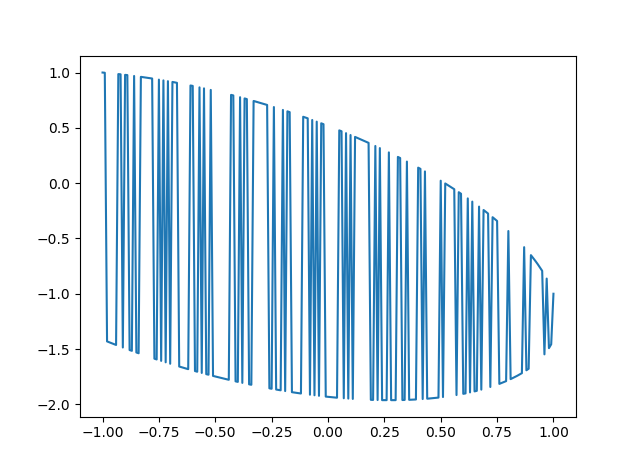
\includegraphics[width=3in] {SVM-figures/Fig5.png}
\end{figure}
	
}


\frame{
	\frametitle{The power of polynomial kernel} 
\begin{figure}
   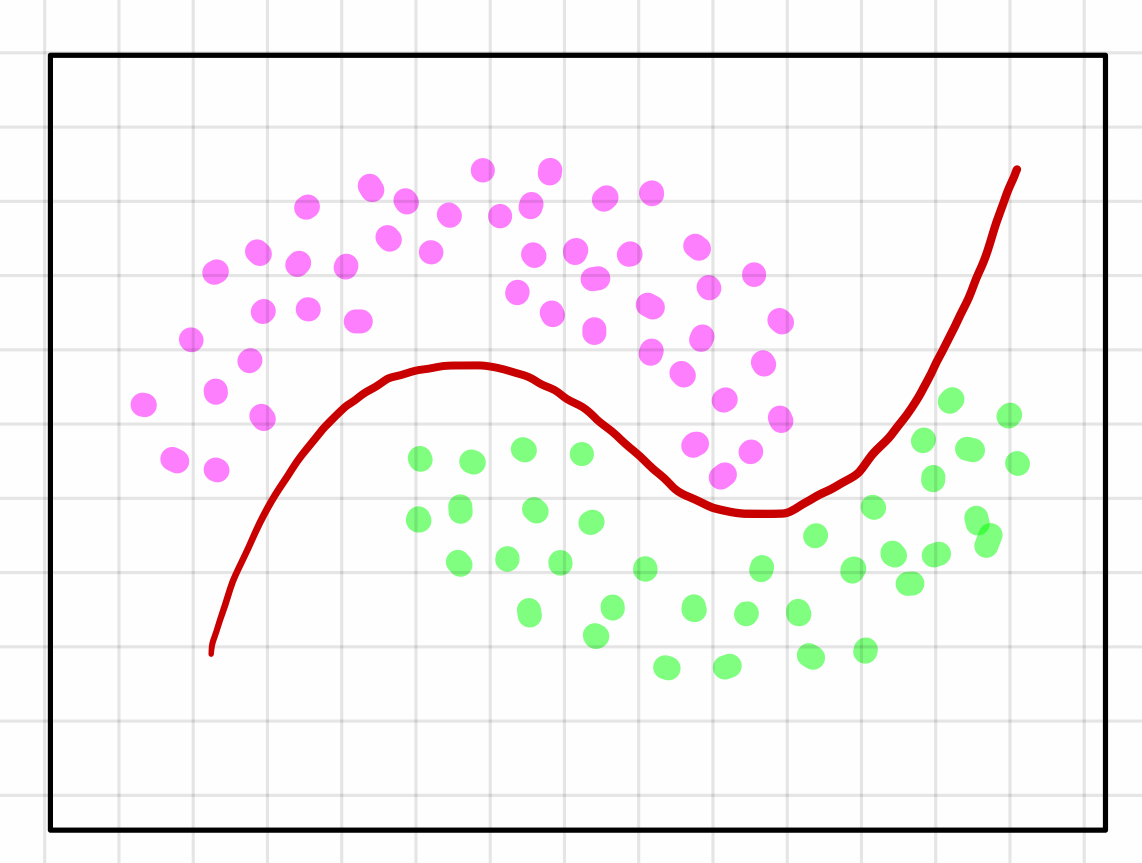
\includegraphics[width=3in] {SVM-figures/pic4.png}
\end{figure}

\begin{itemize}
	\item We can map into a $d$-dimensional feature space. 
\end{itemize}

	
}



\frame{
	\frametitle{The power of polynomial kernel} 
\begin{figure}
   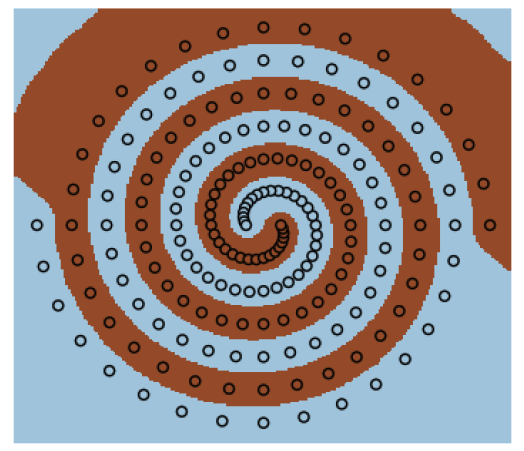
\includegraphics[width=3in] {SVM-figures/Fig1.png}
\end{figure}
	
}

\frame{
	\begin{block}{}
		The requirement of kernel funcitons
 	\end{block}
}

\frame{
	\frametitle{Definition of kernel function} 
	
	\begin{itemize}
		\item A function $k: \mathcal{X}\times \mathcal{X} \rightarrow \mathbb{R}$ is a kernel function if: 
		\begin{itemize}
			\item $k$ is symmetric: $k(x, z) = k(z, x)$. 
			\item For any  $m\in N$ and any $x_{1}, x_{2}, ..., x_{m} \in mathcal{X}$, the matrix $K$ defined by $K_{i,j}  = k(x_{i}, x_{j})$ is positive semidefinite. 
		\end{itemize}
		
	 
	\end{itemize}

\begin{figure}
   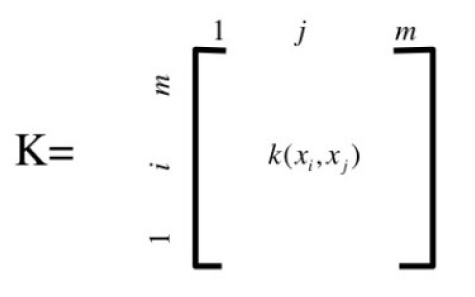
\includegraphics[width=3in] {SVM-figures/Fig2.png}
\end{figure}

}



\frame{
	\begin{block}{}
		Question: Could we map from input space into a feature space with infinite dimension? 
 	\end{block}
}


\frame{
	\frametitle{Map into an infinite dimensional feature space} 
	
\begin{figure}
   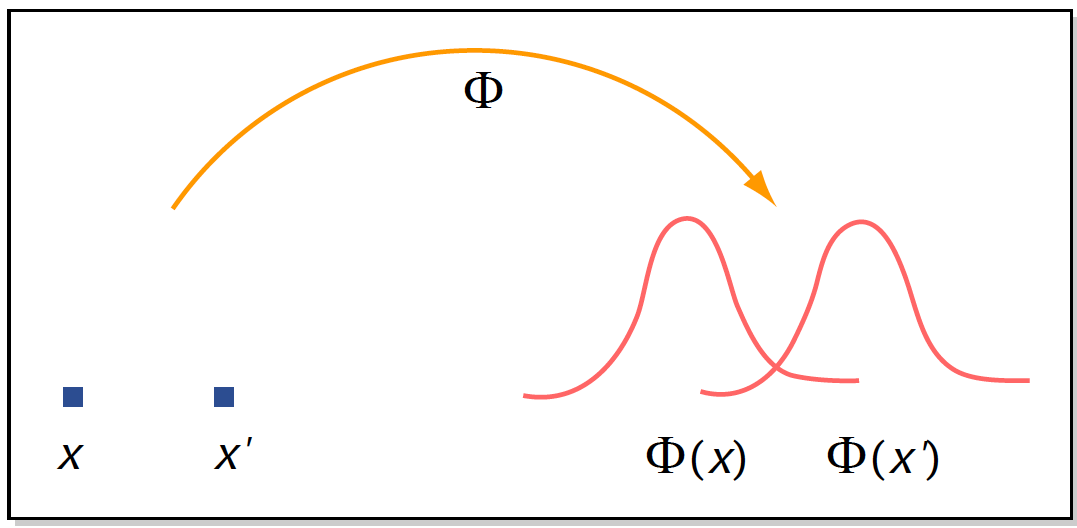
\includegraphics[width=3in] {SVM-figures/Fig3.png}
\end{figure}	 
}

\frame{
	\begin{itemize}
		\item Let's consider the feature space where all elements are functions. 
		\item The span of this space is $\Phi(x_{i}) = k(., x_{i})$. Thus, any element can be represented as: 
		
		\begin{figure}
   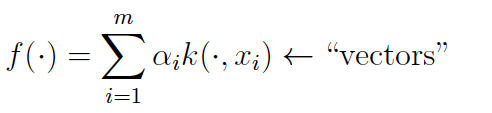
\includegraphics[width=3in] {SVM-figures/Fig6.png}
\end{figure}	 
		\item For two elements 

		\begin{figure}
   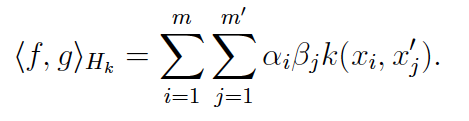
\includegraphics[width=3in] {SVM-figures/Fig7.png}
\end{figure}	 

		
		we define inner product as: 

		\begin{figure}
   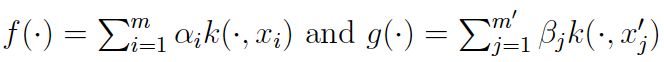
\includegraphics[width=4in] {SVM-figures/Fig8.png}
\end{figure}	 
		 
	\end{itemize}

}



\frame{
	\frametitle{Reproducing kernel Hilbert space}
	
	\begin{itemize}
		\item Now we find a map such that 

	\begin{figure}
   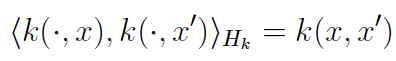
\includegraphics[width=4in] {SVM-figures/Fig9.png}
\end{figure}	 


	\end{itemize}	

}


\frame{
}


\frame{
\begin{Theorem}[Farkas lemma]
Given vectors $\mathbf{a_1, a_{2}, ..., a_{m}, c} \in \mathbb{R}^n$. Then either
\begin{enumerate}
\item  $\mathbf{c} \in \mathbf{C(a_{1}, a_{2},..., a_{m})}$; or 
\item there is a vector $\mathbf{y}\in \mathbb{R}^{n}$ such that for all $i$, $\mathbf{y^T a_i \geq 0}$ but $\mathbf{ y^T c < 0}$.
\end{enumerate}
\end{Theorem}

\begin{figure}
\begin{minipage}{0.45\textwidth}
\begin{tikzpicture}[scale=0.8, auto,swap]
 
\draw[white, fill=green!20] (0,0) -- (2.5, 0) arc (0:45:2.5) -- (0,0); 
\draw[->,  thick] (0,0) -- (2.5,0) node[ultra thick, below] {$\mathbf{a_1}$};
\draw[->,  thick] (0,0) -- (1.73,1.73) node[ultra thick, above] {$\mathbf{a_2}$};
 
\draw[ dashed ] (0, -1.5) -- (0, 1.5);
\draw[ dashed ] (1.2, -1.2) -- (-1.22, 1.21);
 
\node[ thick, blue ] at (2.9, 0.5) {$\mathbf{C(a_1, a_2)}$ };
 
\draw[->, blue, thick] (0,0) -- (2.1, 1.2) node[ultra thick,  right ] {$\mathbf{c}$};

\draw[->, red, thick] (0,0) -- (0.5, 1.5) node[ultra thick,  above ] {$\mathbf{y}$};

\draw[->, red, thick] (0,0) -- (1.5, -0.5) node[ultra thick,  right ] {$\mathbf{y}$};


         
\end{tikzpicture}
\caption{Case 1:  $\mathbf{c} \in \mathbf{C(a_{1}, a_{2})}$}
\end{minipage}
\begin{minipage}{0.45\textwidth}
\begin{tikzpicture}[scale=0.8, auto,swap]
 
\draw[white, fill=green!20] (0,0) -- (2.5, 0) arc (0:45:2.5) -- (0,0); 
\draw[->,  thick] (0,0) -- (2.5,0) node[ultra thick, below] {$\mathbf{a_1}$};
\draw[->,  thick] (0,0) -- (1.73,1.73) node[ultra thick, above] {$\mathbf{a_2}$};
 
\draw[ dashed ] (0, -1.5) -- (0, 1.5);
\draw[ dashed ] (1.2, -1.2) -- (-1.22, 1.21);
 
\node[ thick, blue ] at (2.8, 0.5) {$\mathbf{C(a_1, a_2)}$ };
 
\draw[->, blue, thick] (0,0) -- (1, -1.3) node[ultra thick,  right ] {$\mathbf{c}$};

\draw[->, red, thick] (0,0) -- (0.5, 1.5) node[ultra thick,  above ] {$\mathbf{y}$};


         
\end{tikzpicture}
\caption{Case 2:  $\mathbf{c} \notin \mathbf{C(a_{1}, a_{2})}$}
\end{minipage}
\end{figure}
\begin{itemize}
\item 
Here, $\mathbf{ C(a_1,..., a_m)}$ denotes the cone spanned by $\mathbf{a_1, ..., a_m}$, i.e.  $\mathbf{C(a_1,..., a_m)=\{ x | x=} \sum_{i=1}^m \lambda_i \mathbf{a_i}, \lambda_i \geq 0 \}$.

\end{itemize}
} 


\frame{
\frametitle{}
\begin{Proof} 
\begin{small}
\begin{itemize}
\item Suppose for any vector $\mathbf{y} \in \mathbb{R}^n$, $\mathbf{y^Ta_i\geq 0} \ (i=1,2,...,m)$, we always have $\mathbf{y^T c \geq 0}$. We will show that $\mathbf{c}$ should lie within the cone $\mathbf{C(a_1, a_2,..., a_m)}$. 
\item 
Consider the following {\sc Primal} problem:
\[
\begin{array}{rrrrrrrrl}
 \min & \mathbf{ c^T y } &   &\\
 s.t. & \mathbf{ a_i^T y} & \geq& \mathbf{ 0 } & i=1,2,..., m\\
%      & \mathbf{ y } &\leq\geq &\mathbf{0 } \\
\end{array} \nonumber
\]
\item It is obvious that the {\sc Primal} problem has a feasible solution $\mathbf{ y=0}$, and is bounded since $\mathbf{ c^T y \geq 0}$. 
\item Thus the {\sc Dual} problem also has a bounded optimal solution: 
\[
\begin{array}{rrrrrrrrl}
 \max & 0 &  &  \\
 s.t. & \mathbf{ x^T A^T } &=& \mathbf{c^T } \\
      & \mathbf{ x}  &\geq& \mathbf{0 } \\
\end{array} \nonumber
\]
\item In other words, there exists a vector $\mathbf{ x }$ such that $\mathbf{ c}=\sum_{i=1}^m x_i \mathbf{ a_i}$ and $x_{i} \geq 0$. 
\end{itemize}
\end{small}
\end{Proof}
}



\frame{
	\frametitle{Variants of Farkas' lemma} 
	Farkas' lemma lies at the core of linear optimization. Using Farkas' lemma, we can prove {\sc Separation} theorem, and {\sc MiniMax} theorem in the game theory. 
	
	\begin{Theorem}
	Let $\mathbf{A}$ be an $m\times n$ matrix, and $\mathbf{b} \in \mathbb{R}^{m}$. Then either 
	\begin{enumerate}
	\item $\mathbf{A x = b}$, $\mathbf{x\geq 0}$ has a feasible solution; or
		\item there is a vector $\mathbf{y}\in \mathbb{R}^{m}$ such that   $\mathbf{y^{T} A \geq 0}$ but $\mathbf{y^{T} b  < 0}$. 

		\end{enumerate}
	\end{Theorem} 
}



\frame{
	\frametitle{Variants of Farkas' lemma} 
	\begin{Theorem}
	Let $\mathbf{A}$ be an $m\times n$ matrix, and $\mathbf{b} \in \mathbb{R}^{m}$. Then either 
	\begin{enumerate}
	\item $\mathbf{A x \leq b}$ has a feasible solution; or
	\item there is a vector $\mathbf{y}\in \mathbb{R}^{m}$ such that  $\mathbf{y\geq 0}$, $\mathbf{y^{T} A \geq 0}$ but $\mathbf{y^{T}b < 0}$. 
	\end{enumerate}
	\end{Theorem} 
}


\frame{
	\frametitle{Caratheodory's theorem} 
	\begin{Theorem} 
Given vectors $\mathbf{a_1, a_{2}, ..., a_{m}} \in \mathbb{R}^n$. If $\mathbf{x} \in \mathbf{C(a_{1}, a_{2},..., a_{m})}$, then there is a 
linearly independent vector set of $\mathbf{a_1, a_{2}, ..., a_{m}}$, say $\mathbf{a_1, a_{2}, ..., a_{r}}$, such that $\mathbf{x} \in \mathbf{C(a_{1}, a_{2},..., a_{r})}$. 
\end{Theorem}
} 



\frame{
	\frametitle{{\sc Separation} theorem} 
	
	\begin{Theorem}
		Let $\mathbf{C} \subseteq \mathbb{R}^n$ be a closed, convex set, and let $\mathbf{x} \in \mathbb{R}^n$. If $\mathbf{x} \notin \mathbf{C}$, then there exists a hyperplane separating $\mathbf{x}$ from $\mathbf{C}$. 
	\end{Theorem}
}


\frame{
\begin{block}{}
Application 2: von Neumann's {\sc MiniMax} theorem on game theory 
\end{block}
}

\frame{
	\frametitle{Game theory} 

	\begin{itemize}
		\item Game theory studies  competing and cooperative behaviours among intelligent and rational decision-makers. 
%		\item Originally game theory studies zero-sum games, where one player's gains amount to  other players' losses. 
		\item In 1928, John von Neumann proved the existence of mixed-strategy equilibria in two-person zero-sum games.
		% using Brouwer's fixed-point theorem.
		\item In 1950, John Forbes Nash Jr. developed a criterion of mutual consistency of players' strategies, which applies to a wider range of games than that proposed by J. von Neumann. He proved the existence of Nash equilibrium in every $n$-player, non-zero-sum, non-cooperative game (not just 2-player, zero-sum games). 
		\item Game theory was widely applied in mathematical economics, in biology (e.g., analysis of evolution and stability) and computer science (e.g., analysis of interactive computations and lower bound on the complexity of randomized algorithms, the equivalence between linear program and two-person zero-sum game). 
	\end{itemize}	
}

\frame{	
	\frametitle{Paper-rock-scissors: an example of two-player zero-sum game} 
	
	\begin{itemize}
		\item Paper-rock-scissors is a hand game usually played by two players, denoted as row player and column player: each player selects one of the three hand shapes,  including ``paper", ``rock", and ``scissors"; then the players show their selections simultaneously.
		\item It has two possible outcomes other than tie: one player wins and the other player loses, which can be formally described using the following payoff matrix. 

%\begin{table}[ht]
%%\caption{Multi-column and multi-row table}
%\begin{center}
%\begin{tabular}{|c|c|c|c|c|}
%    \hline
%    \multicolumn{2}{|c|}{\multirow{2}{*}{}}&\multicolumn{3}{c|}{\small Column player}\\
%    \cline{3-5}
%    \multicolumn{2}{|c|}{}& {\small Paper} & {\small Rock} & {\small Scissor} \\
%    \hline
%    \multirow{3}{*}{\small Row player}&  {\small Paper}  & 0 & 1 & -1\\
%    \cline{2-5}
%    & {\small Rock} & -1 & 0 & 1\\
%    \cline{2-5}
%     & {\small Scissor} &  1&  -1 & 0\\
%    \hline
%\end{tabular}
%\end{center}
%\label{tab:multicol}
%\end{table}


\begin{table}[ht]
%\caption{Multi-column and multi-row table}
\begin{center}
\begin{tabular}{|c|c|c|c|}
    \hline
      & \textcolor{blue}{\small Paper} & \textcolor{blue}{\small Rock} & \textcolor{blue}{\small Scissors} \\
    \hline
      \textcolor{red}{\small Paper}  & \textcolor{red}{\small 0},  \textcolor{blue}{\small 0} & \textcolor{red}{\small 1},  \textcolor{blue}{\small -1}  & \textcolor{red}{\small -1},  \textcolor{blue}{\small 1} \\
         \hline 
      \textcolor{red}{\small Rock} & \textcolor{red}{\small -1},  \textcolor{blue}{\small 1} & \textcolor{red}{\small 0},  \textcolor{blue}{\small 0}  & \textcolor{red}{\small 1},  \textcolor{blue}{\small -1}\\
         \hline
     \textcolor{red}{\small Scissors} &  \textcolor{red}{\small 1},  \textcolor{blue}{\small -1}&  \textcolor{red}{\small -1},  \textcolor{blue}{\small 1} & \textcolor{red}{\small 0},  \textcolor{blue}{\small 0} \\
    \hline
\end{tabular}
\end{center}
\label{tab:multicol}
\end{table}


		\item Each player attempts to select appropriate action to maximize his gain.  
	\end{itemize}
}

\frame{
	\frametitle{Matching penny: another example of two-person zero-sum game}
	
	\begin{itemize}
		\item Matching pennies is a game played by two players, namely, row player and column player.  Each player has a penny and  secretly turns it to head or tail. The players then reveal their selections simultaneously. 
		\item If the pennies match, then row player keeps both pennies; otherwise, column player keeps both.  The payoff matrix is as follows. 

\begin{table}[ht]
%\caption{Multi-column and multi-row table}
\begin{center}
\begin{tabular}{|c|c|c|}
    \hline
      & \textcolor{blue}{\small Head} & \textcolor{blue}{\small Tail}  \\
    \hline
      \textcolor{red}{\small Head}  & \textcolor{red}{\small 1},  \textcolor{blue}{\small -1}  & \textcolor{red}{\small -1},  \textcolor{blue}{\small 1} \\
         \hline 
      \textcolor{red}{\small Tail} & \textcolor{red}{\small -1},  \textcolor{blue}{\small 1}   & \textcolor{red}{\small 1},  \textcolor{blue}{\small -1}\\
      \hline
\end{tabular}
\end{center}
\label{tab:multicol}
\end{table}


		\item Each player tries to maximize his gain via making an appropriate selection. 
	\end{itemize}
}

\frame{
	\frametitle{Simultaneous games vs. sequential games}
	\begin{itemize}
		\item \textcolor{red}{\bf Simultaneous games} are games in which all players move \textcolor{blue}{\bf simultaneously}. Thus, no player have information of the others' selections in advance. 
		\item \textcolor{red}{\bf  Sequential games} are games in which the later player has some information, although maybe imperfect,  of previous actions by the other players. A complete plan of action for every stage of the game, regardless of whether the action actually arises in play,  is denoted as \textcolor{red}{\bf a (pure) strategy}. 
		\item \textcolor{red}{\bf Normal form} is used to describe simultaneous games while \textcolor{red}{\bf extensive form} is used to describe sequential games. 
		\item J. von Neumann proposed an approach to transform transform strategies in sequential games into actions in simultaneous games. 
		\item Note that the transformation is one-way, i.e., multiple sequential games might correspond to the same simultaneous game, and it may result in an exponential blowup in the size of the representation. 
	\end{itemize}
}


\frame{
	\frametitle{Normal form}

	\begin{itemize}
			\item A game $\Gamma$ in normal form among $m$ players contains the following items: 
			\begin{itemize}
				\item Each player $k$ has a finite number of \textcolor{red}{\bf pure strategies} $S_k=\{1, 2, ..., n_k\}$.
				\item Each player $k$ is associated with a \textcolor{red}{\bf payoff function} $H_k: S_1\times S_2 \times ... \times S_m \rightarrow \mathbb{R}$. 
			\end{itemize}
		\item To play the game, each player selects a strategy without information of others, and then reveals the selection \textcolor{red}{\bf simultaneously}. The players' gain are calculated using corresponding payoff functions. 
		\item Each player attempts to maximize his gain via selecting an appropriate strategy. 
	\end{itemize}
}

\frame{
	\frametitle{Two-person zero-sum game in normal form } 
\begin{itemize}
	\item In a two-person zero-sum game game $\Gamma$,  a player's gain or less is exactly balanced by the other player's loss or gain, i.e., 
\[	
	H_1(s_1, s_2) + H_2(s_1, s_2) = 0. 
\]	
	\item Thus we can define another function 	
\[	
	H(s_1, s_2) = H_1(s_1, s_2) = -H_2(s_1, s_2)
\] 
	and represent it using a \textcolor{red}{\bf payoff matrix}. 
	
\begin{table}[ht]
%\caption{Multi-column and multi-row table}
\begin{center}
\begin{tabular}{|c|c|c|}
    \hline
      & \textcolor{blue}{\small Head} & \textcolor{blue}{\small Tail}  \\
    \hline
      \textcolor{red}{\small Head}  & \textcolor{red}{\small 1}  & \textcolor{red}{\small -1} \\
         \hline 
      \textcolor{red}{\small Tail} & \textcolor{red}{\small -1}    & \textcolor{red}{\small 1} \\
      \hline
\end{tabular}
\end{center}
\label{tab:multicol}
\end{table}

	\item Row player aims to maximize $H(s_1, s_2)$ by selecting an appropriate strategy $s_1$ while column player aims to minimize $H(s_1, s_2)$ by selecting an appropriate strategy $s_2$. 
	\end{itemize}
}



\frame{
	\frametitle{von Neumann's  {\sc MiniMax}  theorem: motivation } 

	\begin{itemize}
		\item When analyzing a two-person zero-sum game $\Gamma$, von Neumann noticed that the difficulty comes from the difference between games and ordinary optimization problems:   row player tries to maximize $H(s_1, s_2)$; however, he can control $s_1$ only as he has no information of the other player's selection $s_2$, and so does  column player. 
		\item Thus von Neumann suggested to investigate two auxiliary games without this difficulty, denoted as $\Gamma_1$ and $\Gamma_2$, before attacking the challenging game $\Gamma$. 
			\begin{enumerate}
				\item $\Gamma_1$: Row player selects a strategy $s_1$ first, and exposes his selection to column player before column player selects a strategy $s_2$. 
				\item  $\Gamma_2$: Column player selects a strategy $s_2$ first, and exposes his selection to row player before row player selects a strategy $s_1$. 
			\end{enumerate}
		\item The two auxiliary games are much easier than the original game $\Gamma$, and more importantly, they provide upper and lower bounds for $\Gamma$. 
	\end{itemize}
} 

\frame{
	\frametitle{Auxiliary game $\Gamma_1$} 
	\begin{itemize}
		\item Let's consider column player first. As he knows row player's selection $s_1$, the objective function $H(s_1, s_2)$ becomes an ordinary optimization function over a single variable $s_2$, and column player can simply select a strategy $s_2$ with the minimum objective function value $\min_{s_2} H(s_1, s_2)$. 
		
\begin{table}
\begin{center}
\begin{tabular}{|c|c|c|c|}
    \hline
      & {\small Head} & {\small Tail}  & Row minimum \\
    \hline
      {\small Head}  & -2 &  1 & -2\\
         \hline 
     {\small Tail} & -1 &  2 & $v_1 = -1$\\
         \hline
\end{tabular}
\end{center}
\end{table}
		
		\item Now consider  row player. When he selects a strategy $s_1$, he can definitely predict the selection of column player. Since $\min_{s_2} H(s_1, s_2)$ is an ordinary function over  a single  $s_1$, it is easy for row player to select a strategy $s_1$ with the maximum objective function value 
\[
v_1 = \max_{s_1} \min_{s_2} H(s_1, s_2). 
\]				



	\end{itemize}
} 


\frame{
	\frametitle{Auxiliary game $\Gamma_2$} 
	
	\begin{itemize}
		\item Let's consider row player first. As he knows column player's selection $s_2$, the objective function $H(s_1, s_2)$ becomes an ordinary optimization function over  a single variable $s_1$, and row player can simply select a strategy $s_1$ with the maximum objective function value $\max_{s_1} H(s_1, s_2)$. 
		
\begin{table}
\begin{center}
\begin{tabular}{|c|c|c|}
    \hline
      & {\small Head} & {\small Tail}   \\
    \hline
      {\small Head}  & -2 &  1\\
         \hline 
     {\small Tail} & -1 &  2 \\
         \hline
     {\small Column maximum} & $v_2=-1$ &  2\\
         \hline         
\end{tabular}
\end{center}
\end{table}
		
		\item Now consider  column player. When he selects a strategy $s_2$, he can definitely predict the selection of row player. Since $\max_{s_1} H(s_1, s_2)$ is an ordinary function over  a single  variable $s_2$, it is easy for column player to select a strategy $s_2$ with the minimum objective function value 
\[
	v_2 =  \min_{s_2} \max_{s_1} H(s_1, s_2). 
\]				
	\end{itemize}
} 

\frame{
	\frametitle{$\Gamma_1$ and $\Gamma_2$ bound $\Gamma$}
	
	\begin{itemize}
		\item For row player, it is clearly $\Gamma_1$ is disadvantageous to him as he should expose his selection $s_1$ to column player. 
		\item On the contrary, $\Gamma_2$ is beneficial to row player as he knows column player's selection $s_2$ before making decision. 
		
\begin{table}
\begin{center}
\begin{tabular}{|c|c|c|c|}
    \hline
      & {\small Head} & {\small Tail}  & Row minimum \\
    \hline
      {\small Head}  & -2 &  1 & -2 \\
         \hline 
     {\small Tail} & -1 &  2 & $v_1=-1$\\
         \hline
     {\small Column maximum} & $v_2=-1$ &  2 & \\
         \hline         
\end{tabular}
\end{center}
\end{table}

		\item Thus these two auxiliary games provides lower and upper bounds: 
\[
 v_1 \leq v \leq v_2
\]		
		where $v$ denote row player's gain in the original game $\Gamma$. 
%		\item Actually, the two auxiliary games need not to be explicitly specified if we assume reasonable ``wisdom" of the players: each player knows the other's selection through ``experience" or  ``guess".  
	\end{itemize}
}

\frame{
	\frametitle{Case 1: $v_1 = v_2$} 
		
	\begin{itemize}
		\item For a game with the following payoff matrix, we have $v_1 = v = v_2$ and call this game \textcolor{red}{\bf strictly determined}.

\begin{table}
\begin{center}
\begin{tabular}{|c|c|c|c|}
    \hline
      & {\small Head} & {\small Tail}  & Row minimum \\
    \hline
      {\small Head}  & -2 &  1 & -2 \\
         \hline 
     {\small Tail} & -1 &  2 & $v_1=-1$\\
         \hline
     {\small Column maximum} & $v_2=-1$ &  2 & \\
         \hline         
\end{tabular}
\end{center}
\end{table}

		\item The saddle point of the payoff matrix $H(s_1, s_2)$ represents a \textcolor{red}{\bf pure strategy equilibrium}. In this equilibrium, each player has nothing to gain by changing only his own strategy. In addition, knowing the opponent's selection will bring no gain. 
		\item von Neumann proved the existence of the optimal strategy in  a perfect information two-person zero-sum game, e.g., chess. L. S. Shapley further showed that a finite two-person zero-sum game has a pure strategy equilibrium if every $2\times 2$ submatrix of the game has a pure strategy equilibrium \cite{Shapley1964}.  
	\end{itemize}
}

\frame{
	\frametitle{Case 2: $v_1 < v_2$} 
	
	\begin{itemize}
		\item In contrast, matching penny does not have a pure strategy equilibrium as   there is no saddle point in the payoff matrix. So does the paper-rock-scissors game. 
		
\begin{table}
\begin{center}
\begin{tabular}{|c|c|c|c|}
    \hline
      & {\small Head} & {\small Tail}  & Row minimum \\
    \hline
      {\small Head}  & 1 &  -1 & -1 \\
         \hline 
     {\small Tail} & -1 &  1 & $v_1=-1$\\
         \hline
     {\small Column maximum} & $v_2=1$ &  1 & \\
         \hline         
\end{tabular}
\end{center}
\end{table}
		
		\item This fact implies that knowing the opponent's selection might bring gain; however, it is impossible to know the opponent's selection as the players reveal their selections simultaneously. In this case, let's play a mixed strategy rather than a pure strategy.
	\end{itemize}

}

\frame{
	\frametitle{From pure strategy to mixed strategy} 
		\begin{itemize}
			\item A \textcolor{red}{\bf mixed strategy} is an assignment of probability to pure strategies, allowing a player to \textcolor{red}{\bf randomly select a pure strategy}. 
			\item Consider the payoff matrix as below. If the row player select strategy $A$ with probability $1$, he is said to play a pure strategy. If he  tosses a coin and select strategy $A$ if the coin lands head and $B$ otherwise, then he is said to play a mixed strategy. 
			
\begin{table}[ht]
%\caption{Multi-column and multi-row table}
\begin{center}
\begin{tabular}{|c|c|c|}
    \hline
      & \textcolor{blue}{\small A} & \textcolor{blue}{\small B}  \\
    \hline
      \textcolor{red}{\small A}  & \textcolor{red}{\small 1} & \textcolor{red}{\small -1} \\
         \hline 
      \textcolor{red}{\small B} & \textcolor{red}{\small -1}  & \textcolor{red}{\small 1}\\
      \hline
\end{tabular}
\end{center}
\label{tab:multicol}
\end{table}

		\end{itemize}
} 

\frame{
	\frametitle{Two types of interpretation of mixed strategy}					\begin{itemize}
					\item From a player's viewpoint: J. von Neumann described the motivation underlying the introduction of mixed strategy as follows: since it is impossible to exactly know opponent's selection, a player could switch to \textcolor{red}{\bf protect himself by ``randomly selecting his own strategy"}, making it difficult for the opponent to know the player's selection. However, this interpretation came under heavy fire for lacking of behaviour supports: Seldom do people make choices following a lottery.  
					\item From opponent's viewpoint: Robert Aumann and Adam Brandenburger interpreted mixed strategy of a player as \textcolor{red}{\bf opponent's ``belief" of the player's selection}. Thus, Nash equilibrium is an equilibrium of ``belief" rather than actions.   	
				\end{itemize}
}

\frame{
	\frametitle{Existence of mixed strategy equilibrium} 
 	
	\begin{itemize}
		\item Consider a mixed strategy game: row player has $m$ strategies available and he selects a strategy $s_{1}$ according to a distribution $\mathbf{u}$, while  column player has $n$ strategies available and he selects a strategy $s_{2}$ according to a distribution $\mathbf{v}$, i.e., 
\[		
\Pr(s_1=i) = u_{i},  i=1,..., n \quad \Pr(s_2=j) = v_{j},  j=1,..., m 
\]		
Here, $\mathbf{u}$ and $\mathbf{v}$ are  independent.
		\item Thus the expected gain of row player is: 
\[		
		\sum\nolimits_{i=1}^{m}\sum\nolimits_{j=1}^{n} u_{i}  H_{ij}  v_{j} = \mathbf{u^{T} H v}
\]		
		\item row player attempts to minimize $ \mathbf{u^{T} H v}$ via selecting an appropriate  $\mathbf{u}$, while  column player attempts to maximize it via selecting an appropriate  $\mathbf{v}$. 
		\item Now let's consider the two auxiliary games $\Gamma_{1}$ and $\Gamma_{2}$ again and answer the following questions: what happens if row player exposes his mixed strategy to column player? And if we reverse the order of the players? 
	\end{itemize}
}


\frame{
	\frametitle{von Neumann's  {\sc MiniMax}  theorem [1928] } 
		\begin{itemize}
		\item This question has been answered by the von Neumann's {\sc MiniMax} theorem. 
		\begin{theorem}
\[			\max\limits_{\mathbf{u}} \min\limits_{ \mathbf{v} }   \mathbf{u^{T} H v}  = 
			   \min\limits_{\mathbf{v}} \max\limits_{ \mathbf{u} }   \mathbf{u^{T} H v}
\] 
		\end{theorem}
	
	\item 
	The theorem states that knowing the other player's strategy will bring no gain in a mixed-strategy  zero-sum game, and the order doesn't change the value. 
	\item A \textcolor{red}{\bf mixed-strategy Nash equilibrium}  exists for \textcolor{red}{\bf any two-person zero-sum game} with a finite set of actions. A Nash equilibrium
in a two-player game is a pair of strategies, each of which is a best response
to the other; i.e., each gives the player using it the highest possible payoff,
given the other players' strategy.  
	\end{itemize}
}

\frame{
		\frametitle{von Neumann's  {\sc MiniMax}  theorem: proof} 
		\begin{itemize}
		
		\item Let's consider the auxiliary game $\Gamma_{1}$ first, in which the strategy of row player, i.e., $\mathbf{u}$, was exposed to column player. This is of course  beneficial to column player since he can select the optimal strategy $\mathbf{v}$ to minimize $\mathbf{u^{T} H v}$, which is 
		
\[
	\inf\{ \mathbf{u^{T} H v} | \mathbf{ v\geq 0, 1^{T}v} = 1 \} = \min\limits_{j=1, ..., n} \mathbf{ (u^{T} H) }_{j}
\]
		\item Thus row player should select $\mathbf{u}$ to maximize the above value, which can be formulated as a linear program: 
		
\[
\begin{array}{rllll}
 \max & \min \limits_{j=1, ..., n} \mathbf{(u^{T} H)}_{j} &  &  \\
 s.t. & \mathbf{ 1^T u } &=& 1 \\
      & \mathbf{ u}  &\geq& \mathbf{0 } \\
\end{array} \nonumber
\]
	
	\end{itemize}
	
}

\frame{
	\frametitle{von Neumann's  {\sc MiniMax}  theorem: proof  } 
	
	\begin{itemize}
		\item The linear program can be rewritten as below. 
\[
\begin{array}{rllll}
 \max & s \\ 
% \max\limits_{i=1,...,m} \mathbf{(P^{T} v)}_{i} &  &  \\
 s.t. & \mathbf{ u^T H } &\geq & s\mathbf{1^{T}} \\
      & \mathbf{ 1^T u } &=& 1 \\
      & \mathbf{ u}  &\geq& \mathbf{0 } \\
\end{array} \nonumber
\]	
		\item Similarly we consider the auxiliary game $\Gamma_{2}$ and calculate the optimal strategy $\mathbf{v}$ by solving the following linear program. 
\[
\begin{array}{rllll}
 \min & t \\ 
% \max\limits_{i=1,...,m} \mathbf{(P^{T} v)}_{i} &  &  \\
 s.t. & \mathbf{ H v } &\leq & t\mathbf{1} \\
      & \mathbf{ 1^T v } &=& 1 \\
      & \mathbf{ v}  &\geq& \mathbf{0 } \\
\end{array} \nonumber
\]	
\item These two linear programs are both feasible and form Lagrangian dual. Thus they have the same optimal objective value according to the strong duality property.  
		
	\end{itemize}

}

\frame{
	\frametitle{An example: paper-rock-scissors game} 
	
	\begin{itemize}
		\item For the paper-rock-scissors game, we have the following two linear programs. 
		\begin{itemize}
			\item Linear program for $\Gamma_{1}$: 
\[
\begin{array}{rrrrrrrr}
\max & s & & & & & \\
 s.t. & 0 u_1 &-&  u_2 &+&  u_3 & \geq s  \\
       &    u_1 & + & 0 u_2 &-&  u_3 & \geq s  \\
       &    -u_1 & + &  u_2 &+&  0 u_3 & \geq s  \\
       &    u_1 & + &  u_2 &+&  u_3 & = 1  \\
       &    u_1, & & u_2, & &  u_3 & \geq 0 
\end{array} \nonumber
\] 
			\item Linear program for $\Gamma_{2}$: 
\[
\begin{array}{rrrrrrrr}
\min & t & & & & & \\
 s.t. & 0 v_1 &+&  v_2 &-&  v_3 & \leq t  \\
       &   - v_1 & + & 0 v_2 &+&  v_3 & \leq t  \\
       &    v_1 & - &  v_2 &+&  0 v_3 & \leq t  \\
       &    v_1 & + &  v_2 &+&  v_3 & = 1  \\
       &    v_1, & & v_2, & &  v_3 & \geq 0 
\end{array} \nonumber
\] 
		\end{itemize}
		\item The  mixed strategy equilibrium is $\mathbf{u^{T}} = [\frac{1}{3}, \frac{1}{3}, \frac{1}{3}]$ and $\mathbf{u^{T}} = [\frac{1}{3}, \frac{1}{3}, \frac{1}{3}]$ with the game value $0$. 
	\end{itemize}
}

\frame{
	\frametitle{Comments on the mixed strategy equilibrium by von Neumann}
	\begin{itemize}
		\item Note that a mixed strategy equilibrium always exists no matter whether the payoff matrix $\mathbf{H}$ has a saddle point or not. 
		\item Regardless of column player's selection, row player can select an appropriate strategy to guarantee his gain $v_{1} \geq 0$. 
		\item Regardless of row player's selection, column player can select an appropriate strategy to guarantee row player's gain $v_{1} \leq 0$.
		 \item Using the strategy $\mathbf{u^{T}} = [\frac{1}{3}, \frac{1}{3}, \frac{1}{3}]$, row player can guarantee that he ``won't lose'', i.e., the probability of losing is less than the probability of winning. 
		\item The strategy $\mathbf{u^{T}} = [\frac{1}{3}, \frac{1}{3}, \frac{1}{3}]$ is designed for ``protecting himself'' rather than ``attacking his opponent'', i.e., it cannot be used to benefit from opponent's fault.    
	\end{itemize}
}

\frame{
\begin{block}{}
Application 3: Yao's {\sc MiniMax} principle  [1977]
\end{block}
}

\frame{
	\frametitle{Yao's {\sc MiniMax} principle} 
	
	\begin{itemize}
		\item Consider a problem $\Pi$. Let $\mathcal{A}=\{A_{1}, A_{2}, ..., A_{n}\}$ be algorithms to $\Pi$, and $\mathcal{I}=\{I_{1}, I_{2}, ..., I_{m}\}$ be the inputs with a  given size.  Let $T(A_{i}, I_{j})$ be the running time of algorithm $A_{i}$ on the input $I_{j}$. 

\begin{table}[ht]
%\caption{Multi-column and multi-row table}
\begin{center}
\begin{tabular}{|c|c|c|c|}
    \hline
    \multicolumn{2}{|c|}{\multirow{2}{*}{}}&\multicolumn{2}{c|}{\small Algorithms}\\
    \cline{3-4}
    \multicolumn{2}{|c|}{}&$A_1$&$A_2$\\
    \hline
    \multirow{2}{*}{\small Inputs}&$I_1$&$T_{11}$&$T_{12}$\\
    \cline{2-4}
    &$I_2$&$T_{21}$&$T_{22}$\\
    \hline
\end{tabular}
\end{center}
\label{tab:multicol}
\end{table}	
		\item Thus $\max\limits_{I_{j}\in \mathcal{I}} T(A_{i}, I_{j})$ represents the worst-case time for the deterministic algorithm $A_{i}$. 
		\item For a randomized algorithms, however, it is usually difficult to 
		bound its expected running time on worst-case inputs. 
%		A ``Las Vegas'' algorithm is always correct, but its running time is a random variable. 
		\item Yao's {\sc MiniMax} principle provides a technique to build lower bound for \textcolor{red}{\bf the expected running time of any randomized algorithm on its worst-case input}.  		
	\end{itemize}
}

\frame{
	\frametitle{Expected running time of a randomized algorithm $A_{q}$} 

	\begin{itemize}
		\item A ``Las Vegas'' randomized algorithm can be viewed as a distribution over all deterministic algorithms $\mathcal{A}=\{A_{1}, A_{2}, ..., A_{n}\}$. 
		\item Specifically, let $q$ be a distribution over $\mathcal{A}$, and  $A_{q}$ be a randomized algorithm chosen according to $q$, i.e., $A_{q}$ refers to a deterministic algorithm $A_{i}$ with probability $q_{i}$.
		\item Given a input $I_{j}$, the expected running time of $A_{q}$ can be written as 
\[
	E[ T(A_{q}, I_{j})] = \sum_{i=1}^{n} q_{i} T(A_{i}, I_{j}) 		
\]		
		\item Thus $\max\limits_{I_{j}\in \mathcal{I}} E[ T(A_{q}, I_{j}) ]$ represents the expected running time of $A_{q}$ on its worst-case input. 
	\end{itemize}
}

\frame{
	\frametitle{Expected running time of a deterministic algorithm $A_{i}$ on random input} 
	
	\begin{itemize}
		\item Now consider a deterministic algorithm $A_{i}$ running on random input. 
		\item Let $p$ be a distribution over $\mathcal{I}$, and  $I_{p}$ be a random input chosen from $\mathcal{I}$, i.e., $I_{p}$ refers to $I_{j}$ with probability $p_{j}$. 
		\item Given a deterministic algorithm $A_{i}$, its expected running time on random input $I_{p}$ can be written as
		
		\[
			E[ T(A_{i}, I_{p})] = \sum_{j=1}^{m} p_{j} T(A_{i}, I_{j}) 
		\]
		\item Thus $\min\limits_{A_{i}\in \mathcal{A}} E[T(A_{i}, I_{p})]$ represents the expected running time of the best deterministic algorithm on the random input $I_{p}$.
	\end{itemize}
}

\frame{
	\frametitle{Yao's {\sc MiniMax} principle}
	
	\begin{theorem}
		For any random input $I_{p}$ and randomized algorithm $A_{q}$, 
\[
	\min\limits_{A_{i}\in \mathcal{A}} E[ T(A_{i}, I_{p})] \leq \max\limits_{I_{j}\in \mathcal{I}} E[T(A_{q}, I_{j})]
\]
	\end{theorem}
	
	\begin{itemize}
		\item To establish a lower bound for the expected running time of a randomized algorithm on its worst-case input, it suffices to find an appropriate distribution over inputs
		 and prove that on this random input, no deterministic algorithm can do better than the randomized one. 
		\item The power of this technique lies at the fact that one can choose any distribution over 
		inputs and the lower bound is constructed based on deterministic algorithms. 
	\end{itemize}
}

\frame{
	\frametitle{Yao's {\sc MiniMax} principle: proof} 
	\begin{proof}
		\begin{eqnarray}
			\min\limits_{A_{i}\in \mathcal{A}} E[ T(A_{i}, I_{p})]   
			&\leq& \max\limits_{u\in \Delta_{m}}\min\limits_{A_{i}\in \mathcal{A}} E[ T(A_{i}, I_{u})]  \\	
			&=& \max\limits_{u\in \Delta_{m}}\min\limits_{v\in \Delta_{n}} E[ T(A_{v}, I_{u})]  \\	
			&=& \min\limits_{v\in \Delta_{n}}\max\limits_{u\in \Delta_{m}}  E[ T(A_{v}, I_{u})]  \\
			&=& \min\limits_{v\in \Delta_{n}}\max\limits_{I_{j}\in \mathcal{I}}  E[ T(A_{v}, I_{j})]  \\
			&\leq& \max\limits_{I_{j}\in \mathcal{I}}  E[ T(A_{q}, I_{j})]  	
		\end{eqnarray}
	\end{proof}
	\begin{itemize}
		\item Here, $\Delta_{n}$ denotes the set of $n$-dimensional probability vectors. 
		\item Equation (3) follows by the von Neumann's {\sc MiniMax} theorem. 
	\end{itemize}
}

%\frame{
%	\frametitle{Interpretation in terms of game theory}
%	\begin{itemize}
%		\item Let's consider a mixed-strategy two-person game:  row player selects an input while column player selects a deterministic game, and the payoff is the running time of the selected algorithm on the selected input. 
%		\item column player adopts a mixed strategy $q$ to minimize its payoff, or, equivalently, adopts a randomized algorithm $A_{q}$ to minimize its running time. 
%	\end{itemize}
%}

\frame{
\begin{block}{}
Application 4: Revisiting {\sc ShortestPath } algorithm
\end{block}
}


\frame{
	\frametitle{{\sc ShortestPath} problem} 

\begin{block}{}

{\bf INPUT:} 
$n$ cities, and a collection of roads. A road from city $i$ to $j$ has a distance $d(i, j)$. Two specific cities: $s$ and $t$. 


{\bf OUTPUT: } the shortest path from city $s$ to $t$. 
\end{block}	

\begin{figure}
\begin{tikzpicture}[scale=1., auto,swap]
    % Draw a 7,11 network
    % First we draw the vertices
    \foreach \pos/\name in {{(0,1.5)/s}, {(2,1)/u}, {(2,-1)/v},
                            {(4,-1.5)/t}}
        \node[smallvertex] (\name) at \pos {$\name$};
    % Connect vertices with edges and draw weights
    \foreach \source/ \dest /\weight in {s/u/5, u/t/6,u/v/1,s/v/8,          v/t/2}
        \path[edge, blue] (\source) -- node[weight, right] {\small $\weight$} (\dest);

%    \foreach \source/ \dest /\weight in {s/u/{x_{1}}, u/t/{x_{4}},u/v/{x_{3}},s/v/{x_{2}},          v/t/{x_{5}}}
%        \path[edge, blue] (\source) -- node[weight, left] {$\weight$} (\dest);
%       \draw[dashed, ->] (0,0) arc  (120:60:2);
     \end{tikzpicture}
\end{figure}

}
\frame{
\frametitle{{\sc ShorestPath}  problem:  {\sc Primal} problem  }

\begin{figure}
\begin{tikzpicture}[scale=1., auto,swap]
    % Draw a 7,11 network
    % First we draw the vertices
    \foreach \pos/\name in {{(0,1.5)/s}, {(2,1)/u}, {(2,-1)/v},
                            {(4,-1.5)/t}}
        \node[smallvertex] (\name) at \pos {$\name$};
    % Connect vertices with edges and draw weights
    \foreach \source/ \dest /\weight in {s/u/5, u/t/6,u/v/1,s/v/8,          v/t/2}
        \path[edge, blue] (\source) -- node[weight, right] {\small $\weight$} (\dest);

    \foreach \source/ \dest /\weight in {s/u/{x_{1}}, u/t/{x_{4}},u/v/{x_{3}},s/v/{x_{2}},          v/t/{x_{5}}}
        \path[edge, blue] (\source) -- node[weight, left] {\small $\weight$} (\dest);
%       \draw[dashed, ->] (0,0) arc  (120:60:2);
     \end{tikzpicture}
\end{figure}

\begin{itemize}
\item 
{\sc Primal} problem: set variables for \textcolor{red}{\bf roads} (Intuition: $x_i=0/1$ means whether edge $i$ appears in the shortest path), and a constraint means that {\it ``we enter a node through an edge and leaves it through another edge''}. 
\begin{small}
\[
\begin{array}{rrrrrrrrrrll}
 \min &5 x_1   &+&  8 x_2   &+& 1 x_3   &+& 6 x_4   &+& 2 x_5 & \\
 s.t. & x_1 &+&  x_2 & &  & &   & & & = 1    & \text{vertex } s \\
      &     & &      & &  &-&   x_4  &-& x_5 & = -1 &\text{vertex } t  \\
      &  -x_1& &     &+& x_3 &+& x_4  & & & =  0  &\text{vertex } u \\
      &      &-& x_2 &-& x_3 & &      &+&x_5 & =  0 &\text{vertex } v  \\
      &   x_1 &,&     x_2 &,&    x_3  &,&    x_4  &,& x_5 & \textcolor{red}{=  0/1} 		
\end{array} \nonumber
\]
\end{small}
\end{itemize}
}

\frame{
\frametitle{{\sc ShorestPath}  problem:  {\sc Primal} problem  }

\begin{figure}
\begin{tikzpicture}[scale=1., auto,swap]
    % Draw a 7,11 network
    % First we draw the vertices
    \foreach \pos/\name in {{(0,1.5)/s}, {(2,1)/u}, {(2,-1)/v},
                            {(4,-1.5)/t}}
        \node[smallvertex] (\name) at \pos {$\name$};
    % Connect vertices with edges and draw weights
    \foreach \source/ \dest /\weight in {s/u/5, u/t/6,u/v/1,s/v/8,          v/t/2}
        \path[edge, blue] (\source) -- node[weight, right] {$\weight$} (\dest);

    \foreach \source/ \dest /\weight in {s/u/{x_{1}}, u/t/{x_{4}},u/v/{x_{3}},s/v/{x_{2}},          v/t/{x_{5}}}
        \path[edge, blue] (\source) -- node[weight, left] {$\weight$} (\dest);
%       \draw[dashed, ->] (0,0) arc  (120:60:2);
     \end{tikzpicture}
\end{figure}

\begin{itemize}
\item 
{\sc Primal} problem: relax the 0/1 integer linear program into linear program by the \textcolor{red}{\bf totally uni-modular} property. 
\begin{small}
\[
\begin{array}{rrrrrrrrrrll}
 \min &5 x_1   &+&  8 x_2   &+& 1 x_3   &+& 6 x_4   &+& 2 x_5 & \\
 s.t. & x_1 &+&  x_2 & &  & &   & & & = 1    & \text{vertex } s \\
      &     & &      & &  &-&   x_4  &-& x_5 & = -1 &\text{vertex } t  \\
      &  -x_1& &     &+& x_3 &+& x_4  & & & =  0  &\text{vertex } u \\
      &      &-& x_2 &-& x_3 & &      &+&x_5 & =  0 &\text{vertex } v  \\
      &   x_1 &,&     x_2 &,&    x_3  &,&    x_4  &,& x_5 & \textcolor{red}{\geq 0} \\ 
       &   x_1 &,&     x_2 &,&    x_3  &,&    x_4  &,& x_5 & \textcolor{red}{\leq 1} 	
\end{array} \nonumber
\]
\end{small}
\end{itemize}
}


\frame{ 
\frametitle{{\sc ShortestPath} problem: {\sc Dual problem} }


\begin{figure}
\begin{tikzpicture}[scale=0.8, auto,swap]
    % Draw a 7,11 network
    % First we draw the vertices
    \foreach \pos/\name in {{(0,1.5)/s}, {(2,1)/u}, {(2,-1)/v},
                            {(4,-1.5)/t}}
        \node[smallvertex] (\name) at \pos {$\name$};
    % Connect vertices with edges and draw weights
    \foreach \source/ \dest /\weight in {s/u/5, u/t/6,u/v/1,s/v/8,          v/t/2}
        \path[edge, blue] (\source) -- node[weight, right] {\small $\weight$} (\dest);

%    \foreach \source/ \dest /\weight in {s/u/{x_{1}}, u/t/{x_{4}},u/v/{x_{3}},s/v/{x_{2}},          v/t/{x_{5}}}
%        \path[edge, blue] (\source) -- node[weight, left] {$\small  \weight$} (\dest);
        
%       \draw[dashed, ->] (0,0) arc  (120:60:2);
   \draw[->, blue, thick] (-0.5, -1.75) -- (-0.5, 2); 
   \node[blue] at (-0.85, 2.2) {$height$};
   \foreach \y/\name in {-1.5/t, -1/v, 1/u, 1.5/s}
   {
   	\draw[blue, thick] (-0.55, \y) -- (-0.45, \y); 
	\node[blue]  at (-0.75, \y) {$y_\name$};
   }
   \end{tikzpicture}
\end{figure}

\begin{itemize}
 \item 
{\sc Dual problem}: set variables for \textcolor{red}{\bf cities}. (Intuition: $y_i$ means the height of city $i$; thus, $y_s - y_t$ denotes the height difference between $s$ and $t$, providing a lower bound of the shortest path length.) 
\begin{small}
\[
\begin{array}{rrrrrrrrrl}
 \max & y_s   &-& y_t  \\
 s.t. & y_s & &      &-& y_u & &     &  \leq 5 & \textcolor{blue}{x_{1}: \text{edge } (s,u)}  \\
      & y_s & &      & &     &-& y_v &  \leq 8 & \textcolor{blue}{x_{2}: \text{edge } (s,v)}   \\
      &     & &      & & y_u &-& y_v &  \leq 1 & \textcolor{blue}{x_{3}: \text{edge } (u,v)}  \\
      &     &-& y_t  & + & y_u & &     &  \leq 6 & \textcolor{blue}{x_{4}: \text{edge } (u,t)}  \\
      &     &-& y_t  & &     &+& y_v &  \leq 2 & \textcolor{blue}{x_{5}: \text{edge } (v,t)}  \\
\end{array} \nonumber
\]
\end{small}
% \item Complementary slackness: an edge used in shortest path $x_i > 0$ $\Leftrightarrow$ equality in dual problem. 
\end{itemize}
}

\frame{
\begin{block}{}
{\sc Dual simplex} method  
\end{block}
}

\frame{
	\frametitle{Revisiting {\sc Primal Simplex} algorithm } 
\begin{itemize}
	\item  Consider the following {\sc Primal}  problem {\bf P}: 
			\begin{small}
\[
\begin{array}{rrrrrrrrrrrrl}
 \min &  x_1     &+&  14 x_2    &+& 6 x_3 \\
 s.t. &   x_1     &+&     x_2    &+& x_3 & \leq & 4   \\
      &   x_1     & &            & &     & \leq & 2   \\
      &           & &            & &  x_3& \leq & 3   \\
      &           & &   3x_2     &+&  x_3& \leq & 6   \\
      &   x_1     &,&   x_2      &,&  x_3& \geq & 0   
\end{array} \nonumber
\]
		\end{small}
		\item  {\sc Primal} simplex tabular: 
		\begin{scriptsize}
	\begin{table}
{
\begin{tabular}{r|rrrrrrr}\hline
  & \textcolor{black}{$x_1$} & $x_2$ & $x_3$ & \textcolor{blue}{$x_4$} & \textcolor{blue}{$x_5$} & \textcolor{blue}{$x_6$} & \textcolor{blue}{$x_7$}\\
\hline
 -z= 0 & $\overline{c_1}$= \textcolor{black}{1}  & $\overline{c_2}$=14 & $\overline{c_3}$=6 & $\overline{c_4}$=0 & $\overline{c_5}$=0 & $\overline{c_6}$=0 & $\overline{c_7}$=0 \\
 \hline
 $\mathbf{x_{B1}} = b_1'$=4 & \textcolor{black}{1} & 1 & 1 & \textcolor{blue}{1} & \textcolor{blue}{0} & \textcolor{blue}{0} & \textcolor{blue}{0} \\
 $\mathbf{x_{B2}} = b_2'$=2 & \textcolor{black}{1} & 0 & 0 & \textcolor{blue}{0} & \textcolor{blue}{1} & \textcolor{blue}{0} & \textcolor{blue}{0} \\
 $\mathbf{x_{B3}} = b_3'$=3 & \textcolor{black}{0} & 0 & 1 & \textcolor{blue}{0} & \textcolor{blue}{0} & \textcolor{blue}{1} & \textcolor{blue}{0} \\
 $\mathbf{x_{B4}} = b_4'$=6 & \textcolor{black}{0} & 3 & 1 & \textcolor{blue}{0} & \textcolor{blue}{0} & \textcolor{blue}{0} & \textcolor{blue}{1} \\
\hline
\end{tabular}
} %{}%
\end{table}
\end{scriptsize}
\item Primal variables: $\mathbf{x}$; Feasible: $\mathbf{ B^{-1} b \geq 0}$.
\item A basis $\mathbf{B}$ is  called \textcolor{red}{\bf primal feasible} if all elements in $\mathbf{B^{-1}b}$ (the first column except for $-z$) are non-negative. 

\end{itemize} 
}

\frame{
	\frametitle{Revisiting {\sc Primal Simplex} algorithm cont'd } 
\begin{itemize}
	\item  Now let's consider the  {\sc Dual}  problem {\bf D}: 
			\begin{small}
\[
\begin{array}{rrrrrrrrrrrrl}
 \max &  4y_1 &+&   2y_2    &+& 3y_3 &+& 6y_4&      &\\
 s.t.    &   y_1  &+&     y_2    & &           &   &             &\leq & 1   \\
         &   y_1  &   &               &  &          &+&  3y_4   & \leq & 14   \\
         &   y_1   & &                &+&  y_3  &+& y_4      & \leq & 6   \\
          &   y_1  &,&   y_2       &,&  y_3   &,&  y_4      & \leq & 0   
\end{array} \nonumber
\]
		\end{small}
		\item  {\sc Primal} simplex tabular: 
		\begin{scriptsize}
	\begin{table}
{
\begin{tabular}{r|rrrrrrr}\hline
  & \textcolor{black}{$x_1$} & $x_2$ & $x_3$ & \textcolor{blue}{$x_4$} & \textcolor{blue}{$x_5$} & \textcolor{blue}{$x_6$} & \textcolor{blue}{$x_7$}\\
\hline
 -z= 0 & $\overline{c_1}$= \textcolor{black}{1}  & $\overline{c_2}$=14 & $\overline{c_3}$=6 & $\overline{c_4}$=0 & $\overline{c_5}$=0 & $\overline{c_6}$=0 & $\overline{c_7}$=0 \\
 \hline
 $\mathbf{x_{B1}} = b_1'$=4 & \textcolor{black}{1} & 1 & 1 & \textcolor{blue}{1} & \textcolor{blue}{0} & \textcolor{blue}{0} & \textcolor{blue}{0} \\
 $\mathbf{x_{B2}} = b_2'$=2 & \textcolor{black}{1} & 0 & 0 & \textcolor{blue}{0} & \textcolor{blue}{1} & \textcolor{blue}{0} & \textcolor{blue}{0} \\
 $\mathbf{x_{B3}} = b_3'$=3 & \textcolor{black}{0} & 0 & 1 & \textcolor{blue}{0} & \textcolor{blue}{0} & \textcolor{blue}{1} & \textcolor{blue}{0} \\
 $\mathbf{x_{B4}} = b_4'$=6 & \textcolor{black}{0} & 3 & 1 & \textcolor{blue}{0} & \textcolor{blue}{0} & \textcolor{blue}{0} & \textcolor{blue}{1} \\
\hline
\end{tabular}
} %{}%
\end{table}
\end{scriptsize}
\item Dual variables: $\mathbf{ y^T=c_B^T B^{-1} }$; Feasible: $\mathbf{ y^T A  \leq c^T }$. 
\item A basis $\mathbf{B}$ is called  \textcolor{red}{\bf dual feasible} if all elements in $\mathbf{\overline{c^T}=c-c_B^TB^{-1}A=c^T-y^TA}$ (the first row except for $-z$) are non-negative. 

\end{itemize} 
}



\frame{
\frametitle{Another view point of the {\sc Primal Simplex} algorithm }
\begin{itemize}

\item Thus another view point of the {\sc Primal Simplex} algorithm can be described as: 
\begin{enumerate}
\item \textcolor{red}{\bf Starting point:} The {\sc Primal Simplex} algorithm starts with a primal feasible solution ($\mathbf{ x_B = B^{-1}b \geq 0 }$); 
\item \textcolor{red}{\bf Maintenance:} Throughout the process we maintain the primal feasibility and move towards the dual feasibility; 
\item  \textcolor{red}{\bf  Stopping criteria:} $\mathbf{ \overline{c}^T = c^T - c_B^T B^{-1} A \geq 0 }$, i.e., $\mathbf{ y^T A \leq c^T }$. In other words, the iteration process ends when the basis is both primal feasible and dual feasible. 
\end{enumerate}
\end{itemize}
} 

\frame{
\frametitle{{\sc Dual simplex} works in just an opposite fashion}
\begin{itemize}

\item
 {\sc Dual simplex}:
 
 \begin{enumerate}
\item \textcolor{red}{\bf Starting point:} The {\sc Dual Simplex} algorithm starts with a dual feasible solution ($\mathbf{\overline{c}^T \geq 0 }$); 
\item \textcolor{red}{\bf Maintenance:} Throughout the process we maintain the dual feasibility and move towards the dual feasibility; 
\item  \textcolor{red}{\bf Stopping criteria:} $\mathbf{ x_B = B^{-1}b \geq 0 }$. In other words, the iteration process ends when the basis is both primal feasible and dual feasible. 
\end{enumerate}
\end{itemize} 
} 

\frame{
\frametitle{{\sc Primal simplex} vs. {\sc Dual simplex} }
\begin{itemize}  
	\item Both   {\sc primal simplex} and  {\sc dual simplex} terminate at the same condition, i.e. the basis is both primal feasible and dual feasible. 
	\item However, the final objective is achieved  in totally opposite fashions--- the  {\sc primal simplex} method keeps the primal feasibility while the {\sc dual simplex} method keeps the dual feasibility during the pivoting process. 
	\item The  {\sc primal simplex} algorithm \textcolor{red}{\it first selects an entering variable and then determines  the leaving variable}.
	\item In contrast, the {\sc dual simplex} method does the opposite; it  \textcolor{red}{\it first selects a leaving variable and then determines an entering variable}. 
	\end{itemize} 
} 

\frame{
	\frametitle{}
	\begin{footnotesize}
{\sc Dual simplex}$(B_I, z, \mathbf{A, b, c})$
\end{footnotesize}
\begin{algorithmic}[1]
\begin{footnotesize}
%\STATE $( B_{I}, \mathbf{A, b, c}, z)=$ {\sc InitializeSimplex}$\mathbf{(A, b, c)}$; 
\STATE \begin{footnotesize}\textcolor{blue}{//{\sc Dual simplex} starts with a dual feasible basis. Here, $B_I$ contains the indices of the basic variables.}\end{footnotesize} 
\WHILE{ \texttt{TRUE} } 
\IF{ there is no index $l$ $(1\leq l \leq m)$ has $b_{l} < 0$ }
\STATE{ $\mathbf{x}  = ${\sc CalculateX}$(B_I, \mathbf{A, b, c})$;}
\RETURN{$(\mathbf{x}, z)$};
\ENDIF;
\STATE{ choose an index $l$ having $b_{l} < 0$ according to a certain rule; }
\FOR{each index $j$ $(1\leq i \leq n)$ }
\IF{$a_{lj} < 0$} 
\STATE{ $\Delta_{j} = -\frac{c_{j}}{a_{lj}};$ } 
\ELSE
\STATE{ $\Delta_{j} = \infty;$}
\ENDIF
\ENDFOR
\STATE{choose an index $e$ that minimizes $\Delta_{j}$;} 
\IF{ $\Delta_{e} = \infty$ }
\RETURN{\texttt{``no feasible solution''};} 
\ENDIF
\STATE{$(B_{I}, \mathbf{A, b, c}, z ) = $ {\sc Pivot}$( B_{I}, \mathbf{A, b, c}, z, e, l)$;}
\ENDWHILE
\end{footnotesize}
\end{algorithmic}
}

\frame{
\frametitle{An example} 

\begin{itemize}
\item 
Standard form:

\[
\begin{array}{rrrrrrrrrrrrl}
 \min & 5 x_1     &+&  35 x_2    &+& 20 x_3 & & \\
 s.t.  &   x_1     &-&     x_2    &-& x_3 & \leq & -2   \\
      &   -x_1     &-&  3x_2     & &        & \leq & -3   \\
      &   x_1     &,&   x_2      &,&  x_3& \geq & 0   \\
\end{array} \nonumber
\]
\item 
Slack form:
\[
\begin{array}{rrrrrrrrrrrrl}
 \min & 5 x_1     &+&  35 x_2    &+& 20 x_3  & &           & &                    \\
 s.t. &   x_1     &-&     x_2    &-& x_3              &+& x_4   & &                     & = & -2   \\
      &   -x_1     &-&  3x_2      & &          &  &         &+& x_5              & = & -3   \\
      &   x_1     &,&   x_2      &,&  x_3   &, &  x_4 &,& x_5               & \geq & 0   \\
\end{array} \nonumber
\]
\end{itemize}

}


\frame{
\frametitle{Step 1} 

\begin{table}
{
\begin{tabular}{r|rrrrrrr}\hline
  & \textcolor{green}{$x_1$} & $x_2$ & $x_3$ & \textcolor{blue}{$x_4$} & \textcolor{blue}{$x_5$} \\
\hline
 -z= 0 & $\overline{c_1}$= \textcolor{green}{5}  & $\overline{c_2}$=35 & $\overline{c_3}$=20 & $\overline{c_4}$=0 & $\overline{c_5}$=0  \\
 \hline
 $\mathbf{x_{B1}} = b_1'$=-2& \textcolor{green}{1} & -1   & -1 & \textcolor{blue}{1} & \textcolor{blue}{0}  \\
 $\mathbf{x_{B2}} = b_2'$=-3 & \textcolor{red}{-1} & -3 & 0  & \textcolor{blue}{0} & \textcolor{blue}{1}  \\
% $\mathbf{x_{B3}} = b_3'$=3 & \textcolor{black}{0} & 0 & 1 & \textcolor{blue}{0} & \textcolor{blue}{0} & \textcolor{blue}{1} & \textcolor{blue}{0} \\
%$\mathbf{x_{B4}} = b_4'$=6 & \textcolor{black}{0} & 3 & 1 & \textcolor{blue}{0} & \textcolor{blue}{0} & \textcolor{blue}{0} & \textcolor{blue}{1} \\
\hline
\end{tabular}
} %{}%
\end{table}


\begin{itemize}
 \item Basis (in blue): \textcolor{blue}{ $\mathbf{B =\{a_4, a_5 \} }$}
 \item Solution: $\mathbf{x=\left[\begin{array}{c}\mathbf{B^{-1}b}\\\mathbf{0}\end{array}\right]}= [ 0, 0, 0, -2, -3 ]^T$. 
 %(Hint: basis variables $x_4,x_5,x_6,x_7$ take value of $b_1', b_2', b_3', b_4'$, respectively. )
% \item $\lambda_{e}$: is stored in the $e$-th column. (Why? the basis $\mathbf{B}$ forms an identity matrix.)
 \item Pivoting: choose \textcolor{red}{$\mathbf{a_5}$} to leave basis since $b_2' = -3  < 0$; choose \textcolor{green}{$\mathbf{a_1}$}  to enter basis since $\min_{j, a_{2j}<0} \frac{\overline{c}_j }{-a_{2j} } = \frac{ \overline{c}_1 }{-a_{21} }$.
\end{itemize}
}



\frame{
\frametitle{Step 2} 

\begin{table}
{
\begin{tabular}{r|rrrrrrr}\hline
  & \textcolor{blue}{$x_1$} & \textcolor{green}{$x_2$} & $x_3$ & \textcolor{blue}{$x_4$} & \textcolor{black}{$x_5$} \\
\hline
 -z= -15 & $\overline{c_1}$= \textcolor{black}{0}  & $\overline{c_2}$=\textcolor{green}{20} & $\overline{c_3}$=20 & $\overline{c_4}$=0 & $\overline{c_5}$=5  \\
 \hline
 $\mathbf{x_{B1}} = b_1'$=-5& \textcolor{blue}{0} & \textcolor{red}{-4}   & -1 & \textcolor{blue}{1} & \textcolor{black}{1}  \\
 $\mathbf{x_{B2}} = b_2'$=3 & \textcolor{blue}{1} & \textcolor{green}{3} & 0  & \textcolor{blue}{0} & \textcolor{black}{-1}  \\
% $\mathbf{x_{B3}} = b_3'$=3 & \textcolor{black}{0} & 0 & 1 & \textcolor{blue}{0} & \textcolor{blue}{0} & \textcolor{blue}{1} & \textcolor{blue}{0} \\
%$\mathbf{x_{B4}} = b_4'$=6 & \textcolor{black}{0} & 3 & 1 & \textcolor{blue}{0} & \textcolor{blue}{0} & \textcolor{blue}{0} & \textcolor{blue}{1} \\
\hline
\end{tabular}
} %{}%
\end{table}


\begin{itemize}
 \item Basis (in blue): \textcolor{blue}{ $\mathbf{B =\{a_1, a_4 \} }$}
 \item Solution: $\mathbf{x=\left[\begin{array}{c}\mathbf{B^{-1}b}\\\mathbf{0}\end{array}\right]}= [ 3, 0, 0, -5, 0 ]^T$. 
 %(Hint: basis variables $x_4,x_5,x_6,x_7$ take value of $b_1', b_2', b_3', b_4'$, respectively. )
% \item $\lambda_{e}$: is stored in the $e$-th column. (Why? the basis $\mathbf{B}$ forms an identity matrix.)
 \item Pivoting: choose \textcolor{red}{$\mathbf{a_4}$} to leave basis since $b_1' = -5  < 0$; choose \textcolor{green}{$\mathbf{a_2}$}  to enter basis since $\min_{j, a_{1j}<0} \frac{\overline{c}_j }{-a_{1j} } = \frac{ \overline{c}_2 }{-a_{12} }$.
\end{itemize}
}

\frame{
\frametitle{Step 3} 

\begin{table}
{
\begin{tabular}{r|rrrrrrr}\hline
  & \textcolor{blue}{$x_1$} & \textcolor{blue}{$x_2$} & \textcolor{green}{$x_3$} & \textcolor{black}{$x_4$} & \textcolor{black}{$x_5$} \\
\hline
 -z= -40 & $\overline{c_1}$= \textcolor{black}{0}  & $\overline{c_2}$=\textcolor{black}{0} & $\overline{c_3}$=\textcolor{green}{15} & $\overline{c_4}$=5 & $\overline{c_5}$=10  \\
 \hline
 $\mathbf{x_{B1}} = b_1'$=$\frac{5}{4}$& \textcolor{blue}{0} & \textcolor{blue}{1}   & \textcolor{green}{$\frac{1}{4}$} & \textcolor{black}{$-\frac{1}{4}$} & \textcolor{black}{$-\frac{1}{4}$}  \\
 $\mathbf{x_{B2}} = b_2'$=$-\frac{3}{4}$ & \textcolor{blue}{1} & \textcolor{blue}{0} & \textcolor{red}{$-\frac{3}{4}$}  & \textcolor{black}{$\frac{3}{4}$} & \textcolor{black}{$-\frac{1}{4}$}  \\
% $\mathbf{x_{B3}} = b_3'$=3 & \textcolor{black}{0} & 0 & 1 & \textcolor{blue}{0} & \textcolor{blue}{0} & \textcolor{blue}{1} & \textcolor{blue}{0} \\
%$\mathbf{x_{B4}} = b_4'$=6 & \textcolor{black}{0} & 3 & 1 & \textcolor{blue}{0} & \textcolor{blue}{0} & \textcolor{blue}{0} & \textcolor{blue}{1} \\
\hline
\end{tabular}
} %{}%
\end{table}


\begin{itemize}
 \item Basis (in blue): \textcolor{blue}{ $\mathbf{B =\{a_1, a_2 \} }$}
 \item Solution: $\mathbf{x=\left[\begin{array}{c}\mathbf{B^{-1}b}\\\mathbf{0}\end{array}\right]}= [ \frac{5}{4}, -\frac{3}{4}, 0, 0, 0 ]^T$. 
 %(Hint: basis variables $x_4,x_5,x_6,x_7$ take value of $b_1', b_2', b_3', b_4'$, respectively. )
% \item $\lambda_{e}$: is stored in the $e$-th column. (Why? the basis $\mathbf{B}$ forms an identity matrix.)
 \item Pivoting: choose \textcolor{red}{$\mathbf{a_1}$} to leave basis since $b_2' = -\frac{3}{4}  < 0$; choose \textcolor{green}{$\mathbf{a_3}$}  to enter basis since $\min_{j, a_{2j}<0} \frac{\overline{c}_j }{-a_{2j} } = \frac{ \overline{c}_3 }{-a_{23} }$.
\end{itemize}
}


\frame{
\frametitle{Step 4} 

\begin{table}
{
\begin{tabular}{r|rrrrrrr}\hline
  & \textcolor{black}{$x_1$} & \textcolor{blue}{$x_2$} & \textcolor{blue}{$x_3$} & \textcolor{black}{$x_4$} & \textcolor{black}{$x_5$} \\
\hline
 -z= -55 & $\overline{c_1}$= \textcolor{black}{20}  & $\overline{c_2}$=\textcolor{black}{0} & $\overline{c_3}$=\textcolor{black}{0} & $\overline{c_4}$=20 & $\overline{c_5}$=5  \\
 \hline
 $\mathbf{x_{B1}} = b_1'$=$1$& \textcolor{black}{$\frac{1}{3}$} & \textcolor{blue}{1}   & \textcolor{blue}{0} &  \textcolor{black}{0} & \textcolor{black}{$-\frac{1}{3}$}   \\
 $\mathbf{x_{B2}} = b_2'$=$1$ & \textcolor{black}{$-\frac{4}{3}$} & \textcolor{blue}{0} & \textcolor{blue}{1}  & \textcolor{black}{-1} & \textcolor{black}{$\frac{1}{3}$}  \\
% $\mathbf{x_{B3}} = b_3'$=3 & \textcolor{black}{0} & 0 & 1 & \textcolor{blue}{0} & \textcolor{blue}{0} & \textcolor{blue}{1} & \textcolor{blue}{0} \\
%$\mathbf{x_{B4}} = b_4'$=6 & \textcolor{black}{0} & 3 & 1 & \textcolor{blue}{0} & \textcolor{blue}{0} & \textcolor{blue}{0} & \textcolor{blue}{1} \\
\hline
\end{tabular}
} %{}%
\end{table}


\begin{itemize}
 \item Basis (in blue): \textcolor{blue}{ $\mathbf{B =\{a_2, a_3 \} }$}
 \item Solution: $\mathbf{x=\left[\begin{array}{c}\mathbf{B^{-1}b}\\\mathbf{0}\end{array}\right]}= [ 0, 1, 1, 0, 0 ]^T$. 
 %(Hint: basis variables $x_4,x_5,x_6,x_7$ take value of $b_1', b_2', b_3', b_4'$, respectively. )
% \item $\lambda_{e}$: is stored in the $e$-th column. (Why? the basis $\mathbf{B}$ forms an identity matrix.)
 \item Done! 
 \end{itemize}
}





\frame{
\frametitle{When dual simplex method is useful? }
\begin{enumerate}
 \item 
The dual simplex algorithm is most suited for problems for which an  \textcolor{red}{\bf initial dual
feasible solution} is easily available. 
\item It is particularly useful for \textcolor{red}{\bf reoptimizing} a problem
after a constraint has been added or some parameters have been changed so that the
previously optimal basis is no longer feasible. 
%\item Dual simplex algorithm might be useful when the number of constraints is much larger than the number of variables. 
\item Trying dual simplex is particularly useful if your LP appears to be highly degenerate, i.e. there are many vertices of the feasible region for which the associated basis is degenerate. We may find that a large number of iterations (moves between adjacent vertices) occur with little or no improvement.\footnote{\begin{small} References: Operations Research Models and Methods, Paul A. Jensen and Jonathan F. Bard; OR-Notes, J. E. Beasley \end{small}}
\end{enumerate} 

% Choose $A_i$ (row) first: choose row $r$ such that $x_r$ is primal infeasible. 
% 
% Then choose $A_j$ (column): $\max_{j, \lambda_{rj} < 0} \frac{ \lambda_{0j} } { \lambda_{rj} }$ to keep dual feasible. 

}

%\frame{
%\frametitle{An example of {\sc Dual Simplex} method }
%
%
%}


\frame{
\begin{block}{}
 Primal\_Dual: another {\sc Improvment} approach
\end{block}
}

\frame{
	\frametitle{Primal\_Dual method: a brief history } 

\begin{itemize}
	\item In 1955, H. Kuhn proposed the Hungarian method for the {\sc MaxWeightedMatching} problem. This method effectively explores the duality property of linear programming. 
	\item In 1956, G. Dantzig, R. Ford, and D. Fulkerson extended this idea to solve linear programming problems. 
	\item In 1957,  R. Ford, and D. Fulkerson applied this idea to solve network-flow problem and Hitchcock problem. 
	\item In 1957, J. Munkres applied this idea to solve the transportation problem. 
\end{itemize}
}


\frame{
\frametitle{Primal\_Dual method: basic idea } 


} 

\frame{
\frametitle{Primal\_Dual Method } 

\begin{itemize}

\item Primal\_Dual method is a dual method, which exploits the lower bound information in subsequent linear programming operations. 

\item Advantages: 
\begin{enumerate}
 \item 
Unlike dual simplex starting from a \textcolor{red}{\bf dual basic feasible solution}, primal\_dual method requires only a \textcolor{red}{\bf dual feasible solution}. 
\item An optimal solution to $DRP$  usually has combinatorial explanation, especially for graph-theory problems. 
\end{enumerate}

\end{itemize}

\begin{figure}
\begin{tikzpicture}[scale=1., auto,swap]

\def\l{2.5};
\def\h{1.5};
\def\d{0.5};

\draw[thick] (0,0) rectangle (\l,\h);
\draw[thick, ->] (\l, \h*0.5) -- ( \l + \d, \h*0.5);
\node[ultra thick] at (\l*0.5, \h*0.5) {\small Primal $P$};
\node[thick, blue] at (\l*0.5 , -0.25) {$\mathbf{x}$};

\node[thick, red] at (\l + \d + \l + \d*0.2 , \h + 0.25 ) {Step $1$: $\mathbf{y\Rightarrow x}$};


\draw[thick] (0 + \l + \d, 0) rectangle (\l + \l + \d,\h);
\draw[thick, ->] (\l + \l + \d , \h*0.5) -- ( \l + \d + \l + \d, \h*0.5);
\node[ultra thick] at (\l+\d + \l*0.5, \h*0.5) {\small Dual  $D$};
\node[thick, blue] at (\l+\d + \l*0.5, -0.25) {$\mathbf{y}$};

\node[thick, red] at (\l + \d + \l + \d + \l + \d*0.8 , \h + 0.25 ) {Step $2$: $\mathbf{x}\Rightarrow \mathbf{\Delta y}$};


\draw[thick] (0 + \l + \d + \l + \d, 0) rectangle (\l + \l + \d+ \l + \d,\h);
\draw[thick, ->] (\l + \l + \d + \l + \d, \h*0.5) -- ( \l + \d + \l + \d + \l + \d, \h*0.5);
\node[ultra thick, align=center] at (\l+\d + \l+\d + \l*0.5,  \h*0.5) {\small Restricted\\ Primal\\ $RP$};
\node[thick, blue] at (\l+\d + \l+\d + \l*0.5,  -0.25) {$\mathbf{x}$};

\node[thick, red] at (\l+\d + \l+\d + \l*0.5,  -1.1) { Step $3$: $\mathbf{y = y + }\theta \times \mathbf{\Delta y}$};


\draw[thick] (0 + \l + \d + \l + \d + \l + \d, 0) rectangle (\l + \l + \d+ \l + \d + \l + \d,\h);
\node[ultra thick, align=center] at (\l+\d + \l+\d + \l+\d + \l*0.5 , \h*0.5) {\small Dual of $RP$\\ $DRP$};
\node[thick, blue] at (\l+\d + \l+\d + \l+\d + \l*0.5 , -0.25) {$\mathbf{\Delta y}$};

\draw[thick] (\l+\d + \l+\d + \l+\d + \l*0.3 , 0) -- (\l+\d + \l+\d + \l+\d + \l*0.3 , -0.8) -- (\l+\d + \l*0.6, -0.8); 
\draw[thick, ->]  (\l+\d + \l*0.6, -0.8) --  (\l+\d + \l*0.6, 0); 


\end{tikzpicture}
\end{figure}

%
%\begin{figure}
%   \includegraphics[width=3in] {L9-primaldualflowchart.eps}
%\end{figure}

}

\frame{
\frametitle{Basic idea of primal\_dual method} 
\begin{itemize}
\begin{footnotesize}
\item 
Primal P: 
\[
\begin{array}{rrrrrrrrrrrrl}
 \min & c_1x_1    &+&  c_2x_2   &+&  ...&+& c_nx_n    &      &    & \\
 s.t. & a_{11}x_1 &+& a_{12}x_2 &+& ... &+& a_{1n}x_n & = & b_1 & \textcolor{blue}{(y_1)} \\
      & a_{21}x_1 &+& a_{22}x_2 &+& ... &+& a_{2n}x_n & = & b_2 & \textcolor{blue}{(y_2)} \\
      &           & &           & & ... & &           &      &     &  \\
      & a_{m1}x_1 &+& a_{m2}x_2 &+& ... &+& a_{mn}x_n & = & b_m &  \textcolor{blue}{(y_m)}\\
      &       x_1 &,&       x_2 &,& ... &,&       x_n & \geq & 0   &  \\
     \end{array} \nonumber
\]
\item 
Dual D: 
\[
\begin{array}{rrrrrrrrrrrrl}
 \max & b_1y_1    &+&  b_2y_2   &+&  ...&+& b_my_m    &      &    & \\
 s.t. & a_{11}y_1 &+& a_{21}y_2 &+& ... &+& a_{m1}y_m & \leq & c_1 &  \\
      & a_{12}y_1 &+& a_{22}y_2 &+& ... &+& a_{m2}y_m & \leq & c_2 &  \\
      &           & &           & & ... & &           &      &     &  \\
      & a_{1n}y_1 &+& a_{2n}y_2 &+& ... &+& a_{mn}y_m & \leq & c_n & 
%      &       y_1 &,&       y_2 &,&     &,&       y_m & \leq\geq & 0   & \\
     \end{array} \nonumber
\]
 \item 
Basic idea: Suppose we are given a dual feasible solution $\mathbf{y}$. Let's verify whether $\mathbf{y}$ is an optimal solution or not: 
	\begin{enumerate}
	\begin{footnotesize}
	\item If $\mathbf{y}$ is an optimal solution to the dual problem $D$, then  the corresponding primal variables $\mathbf{x}$ should satisfy a restricted primal problem called $RP$; 
	\item Furthermore, even if  $\mathbf{y}$ is not optimal, the solution to the dual of $RP$ (called $DRP$) still provide invaluable information --- it can be used to improve $\mathbf{y}$.  
		\end{footnotesize}
	\end{enumerate}
\end{footnotesize}
\end{itemize}
} 



\frame[allowframebreaks]{
\frametitle{Step 1: $\mathbf{y} \Rightarrow \mathbf{x}$} 
\begin{itemize}
\begin{small}

\item Dual problem D: 
\[
\begin{array}{rrrrrrrrrrrrl}
\max & b_1y_1    &+&  b_2y_2   &+&  ...&+& b_my_m    &      &    & \\
 s.t. & a_{11}y_1 &+& a_{21}y_2 &+& ... &+& a_{m1}y_m & \leq & c_1 &  \textcolor{blue}{('='\Rightarrow x_1 \geq 0 )} \\
      %& a_{12}y_1 &+& a_{22}y_2 &+& ... &+& a_{m2}y_m & \leq & c_2 &  ('='\Rightarrow x_2 \geq 0 )\\
      &           & &           & & ... & &           &      &     &  \\
      & a_{1n}y_1 &+& a_{2n}y_2 &+& ... &+& a_{mn}y_m & \leq & c_n &  \textcolor{blue}{ ('<'\Rightarrow x_n = 0 )}
%      &       y_1 &,&       y_2 &,&     &,&       y_m & \leq\geq & 0   & \\
     \end{array} \nonumber
\]

\item $\mathbf{y}$ provides information of the corresponding primal variables $\mathbf{x}$: 

\begin{enumerate} 
 \item 
Given a dual feasible solution $\mathbf{y}$. Let's check whether $\mathbf{y}$ is optimal solution or not. 
\item If $\mathbf{y}$ is optimal, we have the following restrictions on $\mathbf{x}$: 

  $a_{1i}y_1 + a_{2i}y_2 + ... + a_{mi}y_m  \textcolor{red}{<}   c_i \Rightarrow \textcolor{red}{x_i = 0}$ \\
%   $a_{1i}y_1 + a_{2i}y_2 + ... + a_{mi}y_m  =   c_i \Rightarrow x_i \geq 0$ 

(Reason: complement slackness. An optimal solution $\mathbf{y}$ satisfies $( a_{1i}y_1 + a_{2i}y_2 + ... + a_{mi}y_m  - c_i) \times  x_i = 0$) 
\item 
Let's use $J$ to record the index of \textcolor{red}{\bf tight constraints} where ``\textcolor{red}{=}'' holds. 

 \begin{figure}
 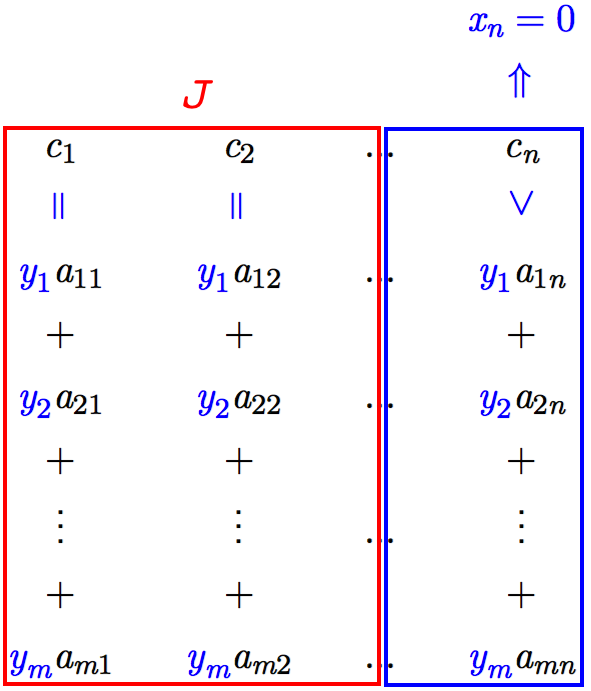
\includegraphics[width=2.5in] {L9-RP.png}
\end{figure}
\item Thus the corresponding primal solution $\mathbf{x}$ should satisfy the following restricted primal (RP): 
\item RP: 
\[
\begin{array}{rrrrrrrrrrrrl}
 %\min & 0& \\
      & a_{11}x_1 &+& a_{12}x_2 &+& ... &+& a_{1n}x_n & = & b_1 &  \\
      & a_{21}x_1 &+& a_{22}x_2 &+& ... &+& a_{2n}x_n & = & b_2 & \\
      &           & &           & & ... & &           &      &     &  \\
      & a_{m1}x_1 &+& a_{m2}x_2 &+& ... &+& a_{mn}x_n & = & b_m & \\
      &           & &           & &     & &       \textcolor{blue}{x_i} & \textcolor{blue}{=} & 0   &\textcolor{blue}{ i\notin J} \\
      &           & &           & &     & &       \textcolor{red}{x_i} & \textcolor{red}{\geq} & 0   & \textcolor{red}{i\in J} 
     \end{array} \nonumber
\]
\item In other words, the optimality of  $\mathbf{y}$ is determined via solving $RP$. 
\end{enumerate}
\end{small}
\end{itemize}
} 


\frame[allowframebreaks]{
\frametitle{But how to solve $RP$?} 
\begin{itemize}
\item 
RP: 
\[
\begin{array}{rrrrrrrrrrrrl}
 %\min & 0& \\
      & a_{11}x_1 &+& a_{12}x_2 &+& ... &+& a_{1n}x_n & = & b_1 &  \\
      & a_{21}x_1 &+& a_{22}x_2 &+& ... &+& a_{2n}x_n & = & b_2 & \\
      &           & &           & & ... & &           &      &     &  \\
      & a_{m1}x_1 &+& a_{m2}x_2 &+& ... &+& a_{mn}x_n & = & b_m & \\
      &           & &           & &     & &       \textcolor{blue}{x_i} & \textcolor{blue}{=} & \textcolor{blue}{0}   &\textcolor{blue}{ i\notin J} \\
      &           & &           & &     & &       \textcolor{red}{x_i} & \textcolor{red}{\geq} & \textcolor{red}{0}   & \textcolor{red}{i\in J} 
\end{array} \nonumber
\]

\item How to solve RP? Recall that $\mathbf{ Ax = b, x\geq 0}$ can be solved via solving an extended LP. 

\item $RP$ (extended through introducing slack variables):
\[
\begin{array}{rrrrrrrllllllllll}
 \min &\epsilon=&s_1    &+s_2   &...&+s_{m} &                   &    &                     &        & \\
 s.t.   &               &s_1    &           &   &            &+a_{11}x_1 &... &+a_{1n}x_{n} & =b_1 & \\
         &               &         &  s_2    &   &            &+a_{21}x_1 &... &+a_{2n}x_{n} & =b_2 & \\
         &               &         &           &...&            &                    &... &                     &          &\\
         &               &         &           &   & s_m    &+a_{m1}x_1 &... &+a_{mn}x_{n} & =b_m & \\
         &               &         &           &    &            &                         &   &\textcolor{blue}{x_i} & \textcolor{blue}{=  0}   &\textcolor{blue}{ i\notin J} \\
         &               &         &           &    &            &                         &    &\textcolor{red}{x_i}  &       \textcolor{red}{\geq  0}   & \textcolor{red}{i\in J} \\
         &               &         &           &     &            &                        &    &             s_i     & \geq 0 &  \forall i  \\
     \end{array} \nonumber
\]
\begin{enumerate}
 \item 
If $\epsilon_{OPT} = 0$, then we find a feasible solution to $RP$, implying that $\mathbf{y}$ is an optimal solution; 
\item 
If $\epsilon_{OPT} > 0$, $\mathbf{y}$ is not an optimal solution. 
\end{enumerate}
\end{itemize} 
} 

\frame[allowframebreaks]{
\frametitle{Step 2: $\mathbf{x} \Rightarrow \mathbf{\Delta{y}}$ } 

\begin{itemize}
\item 
Alternatively, we can solve the dual of $RP$, called $DRP$:
\[
\begin{array}{rrrrrrrrrrrrrrrrrrrrl}
\max & w &=& b_1y_1    &+&  b_2y_2   &+&  ...&+& b_my_m    &      &    & \\
 s.t. & & & a_{11}y_1 &+& a_{21}y_2 &+& ... &+& a_{m1}y_m & \leq & 0 &  \\
      & & & a_{12}y_1 &+& a_{22}y_2 &+& ... &+& a_{m2}y_m & \leq & 0 &  \\
      & & &          & &           & & ... & &           &      &     &  \\
      & & & a_{1|J|}y_1 &+& a_{2|J|}y_2 &+& ... &+& a_{m|J|}y_m & \leq & 0 & \\
      & & &      y_1 &,&       y_2 &,&     &,&       y_m & \leq & 1   & \\
     \end{array} \nonumber
\]

\begin{enumerate}
 \item 
If $w_{OPT} = 0$, $\mathbf{y}$ is an optimal solution
\item 
If $w_{OPT} > 0$, $\mathbf{y}$ is not an optimal solution. However, the optimal solution  still provides useful information --- the optimal solution to $DRP$ can be used to improve $\mathbf{y}$. 
\end{enumerate}
\end{itemize}
} 

\frame{
\frametitle{The difference between $DRP$  and $D$}
\begin{itemize}
\begin{small}
\item Dual problem D: 
\[
\begin{array}{rrrrrrrrrrrrl}
\max & b_1y_1    &+&  b_2y_2   &+&  ...&+& b_my_m    &      &    & \\
 s.t. & a_{11}y_1 &+& a_{21}y_2 &+& ... &+& a_{m1}y_m & \leq & c_1 &   \\
      & a_{12}y_1 &+& a_{22}y_2 &+& ... &+& a_{m2}y_m & \leq & c_2 & \\
      &           & &           & & ... & &           &      &     &  \\
      & a_{1n}y_1 &+& a_{2n}y_2 &+& ... &+& a_{mn}y_m & \leq & c_n & 
%      &       y_1 &,&       y_2 &,&     &,&       y_m & \leq\geq & 0   & \\
     \end{array} \nonumber
\]
\item 
DRP: 
\[
\begin{array}{rrrrrrrrrrrrrrrrrrrrl}
\max & w &=& b_1y_1    &+&  b_2y_2   &+&  ...&+& b_my_m    &      &    & \\
 s.t. & & & a_{11}y_1 &+& a_{21}y_2 &+& ... &+& a_{m1}y_m & \leq & \textcolor{red}{0} &  \\
      & & & a_{12}y_1 &+& a_{22}y_2 &+& ... &+& a_{m2}y_m & \leq & \textcolor{red}{0} &  \\
      & & &          & &           & & ... & &           &      &     &  \\
      & & & a_{1\textcolor{red}{|J|}}y_1 &+& a_{2\textcolor{red}{|J|}}y_2 &+& ... &+& a_{m\textcolor{red}{|J|}}y_m & \leq & \textcolor{red}{0} & \\
      & & &      y_1 &,&       y_2 &,&     &,&       y_m & \leq & \textcolor{red}{1}   & \\
     \end{array} \nonumber
\]
\item How to write $DRP$ from $D$? 
\begin{itemize}
\begin{small}
\item Replacing $c_i$ with $0$;
\item Only $|J|$ restrictions in $DRP$; 
\item An additional restriction: $y_1, y_2, ..., y_m \leq 1$;
\end{small}
\end{itemize}
\end{small}

\end{itemize}


}

\frame[allowframebreaks]{
\frametitle{Step 3: $\mathbf{\Delta {y}} \Rightarrow \mathbf{y} $ } 


Why $\mathbf{\Delta y}$ can be used to improve $\mathbf{y}$? Consider an improved dual solution $\mathbf{y' = y +} \theta \mathbf{ \Delta y}, \theta > 0 $. We have: 
 
\begin{itemize}
\item \textcolor{red}{\bf Objective function:} Since $\mathbf{\Delta y^T b } = w_{OPT}  > 0$,  $\mathbf{y'^T b = y^T b } + \theta w_{OPT}  > \mathbf{ y^T b}$. In other words, $\mathbf{(y+\theta \Delta y)}$ is better than $\mathbf{y}$. 

 \item \textcolor{red}{\bf Constraints:} The dual feasibility requires that: 
\begin{itemize}
 \item For any $ j \in J$,  $a_{1j} \Delta y_1 + a_{2j}\Delta y_2 + ... + a_{mj}\Delta y_m  \leq  0$. Thus we have $\mathbf{y'^Ta_j} = \mathbf{y^Ta_j} + \theta \mathbf{\Delta y^Ta_j} \leq \mathbf{c_j}$ for any $\theta > 0$.  \ \\
 \ \\
 \item For any $j \notin J$, there are two cases: 
 \begin{enumerate}
 \item $\forall j \notin J, a_{1j} \Delta y_1 + a_{2j}\Delta y_2 + ... + a_{mj}\Delta y_m  \leq  0$: 
 
 Thus $\mathbf{y'}$ is feasible for any $\theta > 0$ since for $\forall 1 \leq j \leq n$, 
 
 \begin{eqnarray}
&&  a_{1j}y'_1 + a_{2j}y'_2 + ... + a_{mj}y'_m \\
&=&a_{1j}y_1 + a_{2j}y_2 + ... + a_{mj}y_m \\ 
&+&\theta(a_{1j}\Delta{y_1} + a_{2j}\Delta{y_2} + ... + a_{mj}\Delta{y_m}) \\
&\leq& c_j 
\end{eqnarray}
 Hence dual problem $D$ is unbounded and the primal problem $P$ is infeasible. 
  
 \item $\exists j \notin J, a_{1j} \Delta y_1 + a_{2j}\Delta y_2 + ... + a_{mj}\Delta y_m  >  0$:
  
  We can safely set $\theta \leq \frac{c_j - (a_{1j}y_1 + a_{2j}y_2 + ... + a_{mj}y_m) } {a_{1j}\Delta {y_1} + a_{2j}\Delta {y_2} + ... + a_{mj}\Delta {y_m}} = \frac{ \mathbf{c_j - y^Ta_j} }{ \mathbf{\Delta y^T a_j}  }$ to guarantee that $\mathbf{y'^Ta_j} =\mathbf{y^Ta_j} + \theta \mathbf{\Delta y^Ta_j} \leq \mathbf{c_j}$.  
  
  %(Note: this setting of $\theta$ will make  a constraint $j$ be tight.) 
\end{enumerate}
\end{itemize}
\end{itemize}

}


% \frame[allowframebreaks]{
% 
% 
% $DRP$  specifies a constraint $j$ that can be tighten. Thus, we have a direction to improve $y$ to $y*$, i.e., $y*=y+\theta\overline{y}$. 
% 
% How to set $\theta$ to increase $y^Tb$ while keeping $y$ dual feasible?
% 
% \begin{enumerate}
%  \item increasing $y^Tb \Rightarrow$ $\theta > 0$: Consider objective value: 
% \begin{eqnarray}
% y*^T b &=& y^T b + \theta\overline{y}^Tb \\
%        &=& y^T b + \theta \omega_{OPT}
% \end{eqnarray}
% Thus, in order to increase $y^Tb$, we have $\omega_{OPT} \geq 0 \Rightarrow \theta \geq 0$.
%  
%  \item dual feasible $\Rightarrow$ an upper bound of $\theta$: 
% Consider constraint $j$: 
% \begin{eqnarray}
% &&  a_{1j}y*_1 + a_{2j}y*_2 + ... + a_{mj}y*_m \\
% &=&a_{1j}y_1 + a_{2j}y_2 + ... + a_{mj}y_m \\ 
% &+&\theta(a_{1j}\overline{y_1} + a_{2j}\overline{y_2} + ... + a_{mj}\overline{y_m}) 
% \end{eqnarray}
% 
% \begin{itemize}
%  \item $\forall j, a_{1j}\overline{y_1} + a_{2j}\overline{y_2} + ... + a_{mj}\overline{y_m} \leq 0 $: $y*$ is dual feasible even if $\theta$ is large. Thus, the dual problem $D$ is unbounded, i.e., the primal problem $P$ is infeasible. 
%  
%  \item $\exists j, a_{1j}\overline{y_1} + a_{2j}\overline{y_2} + ... + a_{mj}\overline{y_m} > 0$: we can safely set $\theta \leq \frac{a_{11}y_1 + a_{21}y_2 + ... + a_{m1}y_m}{a_{1j}\overline{y_1} + a_{2j}\overline{y_2} + ... + a_{mj}\overline{y_m}}$. Thus, constraint $j$ is tight now. 
% \end{itemize}
%  
% Remember: 
% \begin{eqnarray}
% a_{11}y_1 + a_{21}y_2 + ... + a_{m1}y_m  &<&  c  . ( '<'. Not \ '\leq' )\\
% a_{11}y_1 + a_{21}y_2 + ... + a_{m1}y_m  &\leq& 0  \\
% \end{eqnarray}
% 
% \end{enumerate}
% 
% }


\frame{
\frametitle{Primal$\_$Dual algorithm}

\begin{small}
\begin{algorithmic} [1]
\STATE Infeasible = ``No''\\
       Optimal = ``No''\\
        $\mathbf{y=y_{0}}$; \qquad //$\mathbf{y_{0}}$ is a feasible solution to the dual problem $D$
\WHILE{TRUE}
\STATE Finding tight constraints index $J$, and set corresponding $x_j = 0 $ for $ j\notin J$. 
\STATE Thus we have a smaller RP.
\STATE Solve DRP. Denote the solution as $\Delta \mathbf{y}$. 
\IF{DRP objective function $w_{OPT} =0$}
\STATE Optimal=``Yes''\\
\RETURN $y$;
\ENDIF
\IF{ $\mathbf{\Delta y^T a_j \leq 0} $ (for all $j \notin J$)}
\STATE Infeasible = ``Yes'';
\RETURN;
\ENDIF
\STATE Set $\theta = \min{ \frac{ \mathbf{c_j - y^Ta_j} }{ \mathbf{\Delta y^T a_j}}}$ for $\mathbf{\Delta y^T a_j}>0$, $j\notin J$.
\STATE Update $\mathbf{ y}$ as  $ \mathbf{ y = y + \theta \Delta y}$;  
\ENDWHILE
\end{algorithmic}
\end{small}
} 

\frame{
\frametitle{Advantages of Primal\_Dual algorithm}

\begin{itemize}

\begin{small}
\item Some facts: 


\begin{itemize}
 \item Primal\_dual algorithm ends if using anti-cycling rule. \\
 (Reason: the objective value $\mathbf{ y^T b }$ increases if there is no degeneracy.)
 \item Both $RP$ and $DRP$ do not explicitly rely on $\mathbf{ c }$.  In fact, the information of $\mathbf{ c }$ is represented in $J$. 
 \item This leads to another advantage of primal\_dual technique, i.e., $RP$ is usually a purely combinatorial problem. Take {\sc ShortestPath} as an example. RP corresponds to a ``connection'' problem. 
 \item More and more constraints become tight in the primal\_dual process. 
\end{itemize}

(See Lecture 10 for a primal\_dual algorithm for {\sc MaximumFlow} problem. )

\end{small}
\end{itemize}

}





\frame{
\begin{block}{}
 {\sc ShortestPath}: Dijkstra's algorithm is essentially Primal$\_$Dual algorithm 
\end{block}
}

\frame{
\frametitle{{\sc ShorestPath} problem }

\begin{figure}
\begin{tikzpicture}[scale=1., auto,swap]
    % Draw a 7,11 network
    % First we draw the vertices
    \foreach \pos/\name in {{(0,1.5)/s}, {(2,1)/u}, {(2,-1)/v},
                            {(4,-1.5)/t}}
        \node[smallvertex] (\name) at \pos {$\name$};
    % Connect vertices with edges and draw weights
    \foreach \source/ \dest /\weight in {s/u/5, u/t/6,u/v/1,s/v/8,          v/t/2}
        \path[edge, blue] (\source) -- node[weight, right] {$\weight$} (\dest);

    \foreach \source/ \dest /\weight in {s/u/{x_{1}}, u/t/{x_{4}},u/v/{x_{3}},s/v/{x_{2}},          v/t/{x_{5}}}
        \path[edge, blue] (\source) -- node[weight, left] {$\weight$} (\dest);
%       \draw[dashed, ->] (0,0) arc  (120:60:2);
     \end{tikzpicture}
\end{figure}

\begin{itemize}
\item 
{\sc Primal} problem: relax the 0/1 integer linear program into linear program by the \textcolor{red}{\bf totally uni-modular} property. 
\begin{small}
\[
\begin{array}{rrrrrrrrrrll}
 \min &5 x_1   &+&  8 x_2   &+& 1 x_3   &+& 6 x_4   &+& 2 x_5 & \\
 s.t. & x_1 &+&  x_2 & &  & &   & & & = 1    & \text{vertex } s \\
      &     & &      & &  &-&   x_4  &-& x_5 & = -1 &\text{vertex } t  \\
      &  -x_1& &     &+& x_3 &+& x_4  & & & =  0  &\text{vertex } u \\
      &      &-& x_2 &-& x_3 & &      &+&x_5 & =  0 &\text{vertex } v  \\
      &   x_1 &,&     x_2 &,&    x_3  &,&    x_4  &,& x_5 & \textcolor{red}{\geq 0} \\ 
       &   x_1 &,&     x_2 &,&    x_3  &,&    x_4  &,& x_5 & \textcolor{red}{\leq 1} 	
\end{array} \nonumber
\]
\end{small}
\end{itemize}
}


\frame{
\frametitle{Dual of {\sc ShortestPath} problem }
\begin{figure}
\begin{tikzpicture}[scale=0.8, auto,swap]
    % Draw a 7,11 network
    % First we draw the vertices
    \foreach \pos/\name in {{(0,1.5)/s}, {(2,1)/u}, {(2,-1)/v},
                            {(4,-1.5)/t}}
        \node[smallvertex] (\name) at \pos {$\name$};
    % Connect vertices with edges and draw weights
    \foreach \source/ \dest /\weight in {s/u/5, u/t/6,u/v/1,s/v/8,          v/t/2}
        \path[edge, blue] (\source) -- node[weight, right] {\small $\weight$} (\dest);

%    \foreach \source/ \dest /\weight in {s/u/{x_{1}}, u/t/{x_{4}},u/v/{x_{3}},s/v/{x_{2}},          v/t/{x_{5}}}
%        \path[edge, blue] (\source) -- node[weight, left] {$\small  \weight$} (\dest);
        
%       \draw[dashed, ->] (0,0) arc  (120:60:2);
   \draw[->, blue, thick] (-0.5, -1.75) -- (-0.5, 2); 
   \node[blue] at (-0.85, 2.2) {$height$};
   \foreach \y/\name in {-1.5/t, -1/v, 1/u, 1.5/s}
   {
   	\draw[blue, thick] (-0.55, \y) -- (-0.45, \y); 
	\node[blue]  at (-0.75, \y) {$y_\name$};
   }
   \end{tikzpicture}
\end{figure}

\begin{itemize}
 \item 
{\sc Dual problem}: set variables for \textcolor{red}{\bf cities}. (Intuition: $y_i$ means the height of city $i$; thus, $y_s - y_t$ denotes the height difference between $s$ and $t$, providing a lower bound of the shortest path length.) 
\begin{small}
\[
\begin{array}{rrrrrrrrrl}
 \max & y_s   &-& y_t  \\
 s.t. & y_s & &      &-& y_u & &     &  \leq 5 & \textcolor{blue}{x_{1}: \text{edge } (s,u)}  \\
      & y_s & &      & &     &-& y_v &  \leq 8 & \textcolor{blue}{x_{2}: \text{edge } (s,v)}   \\
      &     & &      & & y_u &-& y_v &  \leq 1 & \textcolor{blue}{x_{3}: \text{edge } (u,v)}  \\
      &     &-& y_t  & + & y_u & &     &  \leq 6 & \textcolor{blue}{x_{4}: \text{edge } (u,t)}  \\
      &     &-& y_t  & &     &+& y_v &  \leq 2 & \textcolor{blue}{x_{5}: \text{edge } (v,t)}  \\
\end{array} \nonumber
\]
\end{small}
% \item Complementary slackness: an edge used in shortest path $x_i > 0$ $\Leftrightarrow$ equality in dual problem. 
\end{itemize}
}

\frame{ 
\frametitle{A simplified version } 

\begin{figure}
\begin{tikzpicture}[scale=0.8, auto,swap]
    % Draw a 7,11 network
    % First we draw the vertices
    \foreach \pos/\name in {{(0,1.5)/s}, {(2,1)/u}, {(2,-1)/v},
                            {(4,-1.5)/t}}
        \node[smallvertex] (\name) at \pos {$\name$};
    % Connect vertices with edges and draw weights
    \foreach \source/ \dest /\weight in {s/u/5, u/t/6,u/v/1,s/v/8,          v/t/2}
        \path[edge, blue] (\source) -- node[weight, right] {\small $\weight$} (\dest);

%    \foreach \source/ \dest /\weight in {s/u/{x_{1}}, u/t/{x_{4}},u/v/{x_{3}},s/v/{x_{2}},          v/t/{x_{5}}}
%        \path[edge, blue] (\source) -- node[weight, left] {$\small  \weight$} (\dest);
        
%       \draw[dashed, ->] (0,0) arc  (120:60:2);
   \draw[->, blue, thick] (-0.5, -1.75) -- (-0.5, 2); 
   \node[blue] at (-0.85, 2.2) {$height$};
   \foreach \y/\name in {-1.5/t, -1/v, 1/u, 1.5/s}
   {
   	\draw[blue, thick] (-0.55, \y) -- (-0.45, \y); 
	\node[blue]  at (-0.75, \y) {$y_\name$};
   }
   \end{tikzpicture}
\end{figure}

\begin{itemize}
 \item 
{\sc Dual problem}: simplify by setting  $y_{t} =0$ (and remove the 2nd constraint in the primal problem $P$, accordingly)
\begin{small}
\[
\begin{array}{rrrrrrrrrl}
 \max & y_s   & &   \\
 s.t. & y_s & &      &-& y_u & &     &  \leq 5 & \textcolor{blue}{x_{1}: \text{edge } (s,u)}  \\
      & y_s & &      & &     &-& y_v &  \leq 8 & \textcolor{blue}{x_{2}: \text{edge } (s,v)}   \\
      &     & &      & & y_u &-& y_v &  \leq 1 & \textcolor{blue}{x_{3}: \text{edge } (u,v)}  \\
      &     & &    &   & y_u & &     &  \leq 6 & \textcolor{blue}{x_{4}: \text{edge } (u,t)}  \\
      &     & &   & &     & & y_v &  \leq 2 & \textcolor{blue}{x_{5}: \text{edge } (v,t) } \\
\end{array} \nonumber
\]
\end{small}
% \item Complementary slackness: an edge used in shortest path $x_i > 0$ $\Leftrightarrow$ equality in dual problem. 
\end{itemize}
}

\frame[allowframebreaks]{ 
\frametitle{Iteration 1 } 
\begin{small}
\begin{itemize}
 \item Dual feasible solution:  $\mathbf{ y^T = (0, 0, 0) }$.  Let's check the constraints in $D$: 
 \begin{small}
\[
\begin{array}{rrrrrrrrrrl}
 & y_s & &      &-& y_u & &     &  \textcolor{blue}{<}& 5 &  \textcolor{blue}{\Rightarrow  x_{1}  = 0}   \\
 & y_s & &      & &     &-& y_v &   \textcolor{blue}{<}&  8 & \textcolor{blue}{\Rightarrow  x_{2}  = 0}  \\
  &     & &      & & y_u &-& y_v &   \textcolor{blue}{<}&  1 & \textcolor{blue}{\Rightarrow  x_{3}  = 0} \\
 &     & &    &   & y_u & &     &   \textcolor{blue}{<}&  6 & \textcolor{blue}{\Rightarrow  x_{4}  = 0}  \\
 &     & &   & &     & & y_v &   \textcolor{blue}{<}&  2 & \textcolor{blue}{\Rightarrow  x_{5}  = 0}  
\end{array} \nonumber
\]
\end{small}
 \item Identifying tight constraints in $D$:  \textcolor{red}{$J=\Phi$}, implying that $x_1,x_2,x_3,x_4,x_5=0$. 
 \item RP: 
\[
\begin{array}{rrrrrrrrrrrrrrrrrl}
 \min & s_1 &+s_2 & +s_3 &     &        &    &     &   & \\
 s.t. & s_1 &     &     & \textcolor{blue}{+x_1}  & \textcolor{blue}{+x_2} &    &     &   & = 1    & \text{node }s  \\
%       &     & &      & &  &-&   x_4  &-& x_5 & = -1 &\text{vertex t}  \\
     &      &s_2     &             &  \textcolor{blue}{-x_1}  &     & \textcolor{blue}{+x_3}  &  \textcolor{blue}{+x_4}     &  & =  0  & \text{node }u\\
     &      &          & s_3       &     & \textcolor{blue}{-x_2}    & \textcolor{blue}{-x_3}  &      & \textcolor{blue}{+x_5} & =  0 & \text{node }v \\
     & s_1, &s_2, &s_3,  &      &          &         &         &     & \geq 0 \\
     &         &       &         &  \textcolor{blue}{x_1,} &    \textcolor{blue}{ x_2,} &    \textcolor{blue}{x_3,} &   \textcolor{blue}{x_4,} & \textcolor{blue}{x_5} & \textcolor{blue}{= 0} \\ 	
\end{array} \nonumber
\]
% \[
% \begin{array}{rrrrrrrrrrrrrrrrrrrl}
%  \min &  & \epsilon=s_1    &+&  s_2   &+&  ...&+&  s_{3}    &      &    & \\
%  s.t. &   s_1& &           & &  & & ... & &             & = &   1 &  \\
%       &   s_2& &           & &  & & ... & &             & = &   0 &  \\
% %       &       & &          & & ... & &           &      &     &  \\
%       &   s_3& &           & &  & &     & &             & = &   0 & \\
%       &       & &          & &     & &       s_i & \geq & 0   & \forall i\\
%      \end{array} \nonumber
% \]
%   
\item $DRP$:   
\[
\begin{array}{rrrrrrrrrl}
 \max & y_s &      & &            &\\
s.t. & y_s  &      & &     \leq 1 &  \\
     &      & y_u  & &     \leq 1 &  \\
     &      &      & & y_v \leq 1 &  \\  
\end{array} \nonumber
\]

  
%\[
%\begin{array}{rrrrrrrrrl}
% \max & y_s &      & &            &\\
%s.t. & y_s  &      & &     \leq 1 &  \\
%     &      & y_u  & &     \leq 1 &  \\
%     &      &      & & y_v \leq 1 &  \\  
%\end{array} \nonumber
%\]


\item  Solve $DRP$  using combinatorial technique: optimal solution  $\Delta \mathbf{y^T} = (1, 0, 0)$. \textcolor{green}{{\it Note: the optimal solution  is not unique}}

\item Step length $\theta$: $\theta = \min \{ \frac{ \mathbf{c_1 - y^Ta_1} }{ \mathbf{\Delta y^T a_1}  }, \frac{ \mathbf{c_2 - y^Ta_2} }{ \mathbf{\Delta y^T a_2}  }  \} = \min\{ 5, 8\} = 5$

\item Update $\mathbf{y}$: $\mathbf{y^T=y^T}+\theta \Delta \mathbf{y^T}  = (5, 0, 0)$. 


\begin{figure}
\begin{tikzpicture}[scale=0.8, auto,swap]

    \def\ys{2};
    \def\yu{0};
    \def\yv{0};
    \def\yt{0};
    
    \foreach \pos/\name in {{(0,\ys)/s}, {(0,\yu)/u}, {(1.3,\yv)/v}, {(3,\yt)/t}}
        \node[smallvertex] (\name) at \pos {$\name$};

    \foreach \source/ \dest /\weight in {s/u/5,s/v/8}
        \path[edge, blue] (\source) -- node[weight, right] {\small $\weight$} (\dest);
    \foreach \source/ \dest /\weight in { u/v/1, v/t/2}
        \path[edge, blue] (\source) -- node[weight, below] {\small $\weight$} (\dest);
    \draw[->, thick, blue] (u) to[out=-60, in=240] node[below]{\small $6$} (t);

   \draw[->, blue, thick] (-0.5, -0.2) -- (-0.5, 2.3); 
   \node[blue] at (-1.2, 2.5) {$height$};
   
    	\draw[blue, thick] (-0.55, \yu) -- (-0.45, \yu); 
	\node[blue]  at (-2.3, \yu) {$y_u=y_v=y_t=0$};
  
    	\draw[blue, thick] (-0.55, \ys) -- (-0.45, \ys); 
	\node[blue]  at (-1.2, \ys) {$y_s=5$};

   \end{tikzpicture}
\end{figure}


\item From the point of view of Dijkstra's algorithm: 
\begin{itemize}
\item Optimal solution  to $DRP$ is $\Delta \mathbf{y^T} = (1, 0, 0)$: the explored vertex set $S = \{s\}$ in Dijkstra's algorithm. In fact, $DRP$ is solved via identifying the nodes reachable from $s$.
\item Step length  $\theta = \min \{ \frac{ \mathbf{c_1 - y^Ta_1} }{ \mathbf{\Delta y^T a_1}  }, \frac{ \mathbf{c_2 - y^Ta_2} }{ \mathbf{\Delta y^T a_2}  }  \} = \min\{ 5, 8\} = 5$: finding the closest vertex to the nodes in $S$ via comparing all edges going out from $S$. 
\end{itemize}

\end{itemize}

\end{small}

}


\frame[allowframebreaks]{ 
\frametitle{Iteration 2 } 
\begin{small}
\begin{itemize}
 \item Dual feasible solution:  $\mathbf{ y^T = (5, 0, 0) }$.  Let's check the constraints in $D$: 
 \begin{small}
\[
\begin{array}{rrrrrrrrrrl}
 & y_s & &      &-& y_u & &     &  \textcolor{red}{=}& 5 &  \\
 & y_s & &      & &     &-& y_v &   \textcolor{blue}{<}&  8 & \textcolor{blue}{\Rightarrow  x_{2}  = 0}  \\
  &     & &      & & y_u &-& y_v &   \textcolor{blue}{<}&  1 & \textcolor{blue}{\Rightarrow  x_{3}  = 0} \\
 &     & &    &   & y_u & &     &   \textcolor{blue}{<}&  6 & \textcolor{blue}{\Rightarrow  x_{4}  = 0}  \\
 &     & &   & &     & & y_v &   \textcolor{blue}{<}&  2 & \textcolor{blue}{\Rightarrow  x_{5}  = 0}  
\end{array} \nonumber
\]
\end{small}
 \item Identifying tight constraints in $D$:  \textcolor{red}{$J=\{ 1\}$}, implying that $x_2,x_3,x_4,x_5=0$. 
 \item RP: 
\[
\begin{array}{rrrrrrrrrrrrrrrrrl}
 \min & s_1 &+s_2 & +s_3 &     &        &    &     &   & \\
 s.t. & s_1 &     &     & \textcolor{red}{+x_1}  & \textcolor{blue}{+x_2} &    &     &   & = 1    & \text{node }s  \\
%       &     & &      & &  &-&   x_4  &-& x_5 & = -1 &\text{vertex t}  \\
     &      &s_2     &             &  \textcolor{red}{-x_1}  &     & \textcolor{blue}{+x_3}  &  \textcolor{blue}{+x_4}     &  & =  0  & \text{node }u\\
     &      &          & s_3       &     & \textcolor{blue}{-x_2}    & \textcolor{blue}{-x_3}  &      & \textcolor{blue}{+x_5} & =  0 & \text{node }v \\
     & s_1, &s_2, &s_3,  &      &          &         &         &     & \geq 0 \\
     &         &       &         &    &    \textcolor{blue}{ x_2,} &    \textcolor{blue}{x_3,} &   \textcolor{blue}{x_4,} & \textcolor{blue}{x_5} & \textcolor{blue}{= 0} \\ 	
\end{array} \nonumber
\]
% \[
% \begin{array}{rrrrrrrrrrrrrrrrrrrl}
%  \min &  & \epsilon=s_1    &+&  s_2   &+&  ...&+&  s_{3}    &      &    & \\
%  s.t. &   s_1& &           & &  & & ... & &             & = &   1 &  \\
%       &   s_2& &           & &  & & ... & &             & = &   0 &  \\
% %       &       & &          & & ... & &           &      &     &  \\
%       &   s_3& &           & &  & &     & &             & = &   0 & \\
%       &       & &          & &     & &       s_i & \geq & 0   & \forall i\\
%      \end{array} \nonumber
% \]
%   
\item $DRP$:   
\[
\begin{array}{rrrrrrrrrl}
 \max & y_s   & &    \\
 s.t. & y_s &-& y_u  & &     &  \leq 0 &  \\
 %     & y_s & &      &-& y_v &  \leq 0 & \\
      & y_s &,& y_u  &,& y_v &  \leq 1 &  \\
\end{array} \nonumber
\]
  
%\[
%\begin{array}{rrrrrrrrrl}
% \max & y_s &      & &            &\\
%s.t. & y_s  &      & &     \leq 1 &  \\
%     &      & y_u  & &     \leq 1 &  \\
%     &      &      & & y_v \leq 1 &  \\  
%\end{array} \nonumber
%\]


\item  Solve $DRP$  using combinatorial technique: optimal solution  $\Delta \mathbf{y^T} = (1, 1, 0)$. \textcolor{green}{{\it Note: the optimal solution  is not unique}}

\item Step length $\theta$: $\theta = \min \{ 
\frac{ \mathbf{c_2 - y^Ta_2} }{ \mathbf{\Delta y^T a_2}  }, 
\frac{ \mathbf{c_3 - y^Ta_3} }{ \mathbf{\Delta y^T a_3}  },  
\frac{ \mathbf{c_4 - y^Ta_4} }{ \mathbf{\Delta y^T a_4}  }  
\} = \min\{ 3, 1, 6\} = 1$

\item Update $\mathbf{y}$: $\mathbf{y^T=y^T}+\theta \Delta \mathbf{y^T}  = (6, 1, 0)$. 

\begin{figure}
\begin{tikzpicture}[scale=0.8, auto,swap]

    \def\ys{3.3};
    \def\yu{1};
    \def\yv{0};
    \def\yt{0};
    
    \foreach \pos/\name in {{(1,\ys)/s}, {(1,\yu)/u}, {(1,\yv)/v}, {(3,\yt)/t}}
        \node[smallvertex] (\name) at \pos {$\name$};

    \foreach \source/ \dest /\weight in {s/u/5,u/v/1}
        \path[edge, blue] (\source) -- node[weight, right] {\small $\weight$} (\dest);
    \foreach \source/ \dest /\weight in {  v/t/2}
        \path[edge, blue] (\source) -- node[weight, below] {\small $\weight$} (\dest);
    \draw[->, thick, blue] (u) to[out=-10, in=120] node[above]{\small $6$} (t);
    \draw[->, thick, blue] (s) to[out=225, in=135] node[left]{\small $8$} (v);

   \draw[->, blue, thick] (-0.5, -0.2) -- (-0.5, 3.5); 
   \node[blue] at (-1.2, 3.7) {$height$};
   
    	\draw[blue, thick] (-0.55, \yt) -- (-0.45, \yt); 
	\node[blue]  at (-1.7, \yt) {$y_v=y_t=0$};
  
    	\draw[blue, thick] (-0.55, \ys) -- (-0.45, \ys); 
	\node[blue]  at (-1.2, \ys) {$y_s=6$};

    	\draw[blue, thick] (-0.55, \yu) -- (-0.45, \yu); 
	\node[blue]  at (-1.2, \yu) {$y_u=1$};	

   \end{tikzpicture}
\end{figure}


\item From the point of view of Dijkstra's algorithm: 
\begin{itemize}
\item Optimal solution  to $DRP$ is $\Delta \mathbf{y^T} = (1, 1, 0)$: the explored vertex set $S = \{s, u\}$ in Dijkstra's algorithm. In fact, $DRP$ is solved via identifying the nodes reachable from $s$.
\item  Step length   $\theta = \min \{ 
\frac{ \mathbf{c_2 - y^Ta_2} }{ \mathbf{\Delta y^T a_2}  }, 
\frac{ \mathbf{c_3 - y^Ta_3} }{ \mathbf{\Delta y^T a_3}  },  
\frac{ \mathbf{c_4 - y^Ta_4} }{ \mathbf{\Delta y^T a_4}  }  
\} = \min\{ 3, 1, 6\} = 1$: finding the closest vertex to the nodes in $S$ via comparing all edges going out from $S$. 
\end{itemize}

\end{itemize}

\end{small}

}


\frame[allowframebreaks]{ 
\frametitle{Iteration 3 } 
\begin{small}
\begin{itemize}
 \item Dual feasible solution:  $\mathbf{ y^T = (6, 1, 0) }$.  Let's check the constraints in $D$: 
 \begin{small}
\[
\begin{array}{rrrrrrrrrrl}
 & y_s & &      &-& y_u & &     &  \textcolor{red}{=}& 5 &  \\
 & y_s & &      & &     &-& y_v &   \textcolor{blue}{<}&  8 & \textcolor{blue}{\Rightarrow  x_{2}  = 0}  \\
  &     & &      & & y_u &-& y_v &   \textcolor{red}{=}&  1 &  \\
 &     & &    &   & y_u & &     &   \textcolor{blue}{<}&  6 & \textcolor{blue}{\Rightarrow  x_{4}  = 0}  \\
 &     & &   & &     & & y_v &   \textcolor{blue}{<}&  2 & \textcolor{blue}{\Rightarrow  x_{5}  = 0}  
\end{array} \nonumber
\]
\end{small}
 \item Identifying tight constraints in $D$:  \textcolor{red}{$J=\{ 1, 3\}$}, implying that $x_2,x_4,x_5=0$. 
 \item RP: 
\[
\begin{array}{rrrrrrrrrrrrrrrrrl}
 \min & s_1 &+s_2 & +s_3 &     &        &    &     &   & \\
 s.t. & s_1 &     &     & \textcolor{red}{+x_1}  & \textcolor{blue}{+x_2} &    &     &   & = 1    & \text{node }s  \\
%       &     & &      & &  &-&   x_4  &-& x_5 & = -1 &\text{vertex t}  \\
     &      &s_2     &             &  \textcolor{red}{-x_1}  &     & \textcolor{red}{+x_3}  &  \textcolor{blue}{+x_4}     &  & =  0  & \text{node }u\\
     &      &          & s_3       &     & \textcolor{blue}{-x_2}    & \textcolor{red}{-x_3}  &      & \textcolor{blue}{+x_5} & =  0 & \text{node }v \\
     & s_1, &s_2, &s_3,  &      &          &         &         &     & \geq 0 \\
     &         &       &         &    &    \textcolor{blue}{ x_2,} &      &   \textcolor{blue}{x_4,} & \textcolor{blue}{x_5} & \textcolor{blue}{= 0} \\ 	
\end{array} \nonumber
\]
% \[
% \begin{array}{rrrrrrrrrrrrrrrrrrrl}
%  \min &  & \epsilon=s_1    &+&  s_2   &+&  ...&+&  s_{3}    &      &    & \\
%  s.t. &   s_1& &           & &  & & ... & &             & = &   1 &  \\
%       &   s_2& &           & &  & & ... & &             & = &   0 &  \\
% %       &       & &          & & ... & &           &      &     &  \\
%       &   s_3& &           & &  & &     & &             & = &   0 & \\
%       &       & &          & &     & &       s_i & \geq & 0   & \forall i\\
%      \end{array} \nonumber
% \]
%   
\item $DRP$:   
\[
\begin{array}{rrrrrrrrrl}
 \max & y_s   & &    \\
 s.t. & y_s &-& y_u  & &     &  \leq 0 &  \\
     &  & &   y_u   &-& y_v &  \leq 0 & \\
      & y_s &,& y_u  &,& y_v &  \leq 1 &  \\
\end{array} \nonumber
\]
  
%\[
%\begin{array}{rrrrrrrrrl}
% \max & y_s &      & &            &\\
%s.t. & y_s  &      & &     \leq 1 &  \\
%     &      & y_u  & &     \leq 1 &  \\
%     &      &      & & y_v \leq 1 &  \\  
%\end{array} \nonumber
%\]


\item  Solve $DRP$  using combinatorial technique: optimal solution  $\Delta \mathbf{y^T} = (1, 1, 1)$. \textcolor{green}{{\it Note: the optimal solution  is not unique}}

\item Step length $\theta$: $\theta = \min \{ 
\frac{ \mathbf{c_4 - y^Ta_4} }{ \mathbf{\Delta y^T a_4}  } ,
\frac{ \mathbf{c_5 - y^Ta_5} }{ \mathbf{\Delta y^T a_5}  } 
\} = \min\{ 5, 2 \} = 2$

\item Update $\mathbf{y}$: $\mathbf{y^T=y^T}+\theta \Delta \mathbf{y^T}  = (8, 3, 2)$. 

\begin{figure}
\begin{tikzpicture}[scale=0.8, auto,swap]

    \def\ys{3.3};
    \def\yu{1};
    \def\yv{0};
    \def\yt{-1.7};
    
    \foreach \pos/\name in {{(1,\ys)/s}, {(1,\yu)/u}, {(1,\yv)/v}, {(1,\yt)/t}}
        \node[smallvertex] (\name) at \pos {$\name$};

    \foreach \source/ \dest /\weight in {s/u/5,u/v/1}
        \path[edge, blue] (\source) -- node[weight, right] {\small $\weight$} (\dest);
    \foreach \source/ \dest /\weight in {  v/t/2}
        \path[edge, blue] (\source) -- node[weight, right] {\small $\weight$} (\dest);
    \draw[->, thick, blue] (u) to[out=-30, in=30] node[right]{\small $6$} (t);
    \draw[->, thick, blue] (s) to[out=225, in=135] node[left]{\small $8$} (v);

   \draw[->, blue, thick] (-0.5, -2) -- (-0.5, 3.5); 
   \node[blue] at (-1.2, 3.8) {$height$};

    	\draw[blue, thick] (-0.55, \yv) -- (-0.45, \yv); 
	\node[blue]  at (-1.2, \yv) {$y_v=2$};
	   
    	\draw[blue, thick] (-0.55, \yt) -- (-0.45, \yt); 
	\node[blue]  at (-1.2, \yt) {$y_t=0$};
  
    	\draw[blue, thick] (-0.55, \ys) -- (-0.45, \ys); 
	\node[blue]  at (-1.2, \ys) {$y_s=8$};

    	\draw[blue, thick] (-0.55, \yu) -- (-0.45, \yu); 
	\node[blue]  at (-1.2, \yu) {$y_u=3$};	

   \end{tikzpicture}
\end{figure}



\item From the point of view of Dijkstra's algorithm: 
\begin{itemize}
\item Optimal solution  to $DRP$ is $\Delta \mathbf{y^T} = (1, 1, 1)$: the explored vertex set $S = \{s, u, v\}$ in Dijkstra's algorithm. In fact, $DRP$ is solved via identifying the nodes reachable from $s$.
\item  Step length  $\theta = \min \{ 
\frac{ \mathbf{c_4 - y^Ta_4} }{ \mathbf{\Delta y^T a_4}  } ,
\frac{ \mathbf{c_5 - y^Ta_5} }{ \mathbf{\Delta y^T a_5}  } 
\} = \min\{ 5, 2 \} = 2$: finding the closest vertex to the nodes in $S$ via comparing all edges going out from $S$. 
\end{itemize}

\end{itemize}

\end{small}

}



\frame[allowframebreaks]{ 
\frametitle{Iteration 4 } 
\begin{small}
\begin{itemize}
 \item Dual feasible solution:  $\mathbf{ y^T = (8, 3, 2) }$.  Let's check the constraints in $D$: 
 \begin{small}
\[
\begin{array}{rrrrrrrrrrl}
 & y_s & &      &-& y_u & &     &  \textcolor{red}{=}& 5 &  \\
 & y_s & &      & &     &-& y_v &   \textcolor{blue}{<}&  8 & \textcolor{blue}{\Rightarrow  x_{2}  = 0}  \\
  &     & &      & & y_u &-& y_v &   \textcolor{red}{=}&  1 &  \\
 &     & &    &   & y_u & &     &   \textcolor{blue}{<}&  6 & \textcolor{blue}{\Rightarrow  x_{4}  = 0}  \\
 &     & &   & &     & & y_v &   \textcolor{red}{=}&  2 & 
\end{array} \nonumber
\]
\end{small}
 \item Identifying tight constraints in $D$:  \textcolor{red}{$J=\{ 1, 3, 5\}$}, implying that $x_2,x_4 =0$. 
 \item RP: 
\[
\begin{array}{rrrrrrrrrrrrrrrrrl}
 \min & s_1 &+s_2 & +s_3 &     &        &    &     &   & \\
 s.t. & s_1 &     &     & \textcolor{red}{+x_1}  & \textcolor{blue}{+x_2} &    &     &   & = 1    & \text{node }s  \\
%       &     & &      & &  &-&   x_4  &-& x_5 & = -1 &\text{vertex t}  \\
     &      &s_2     &             &  \textcolor{red}{-x_1}  &     & \textcolor{red}{+x_3}  &  \textcolor{blue}{+x_4}     &  & =  0  & \text{node }u\\
     &      &          & s_3       &     & \textcolor{blue}{-x_2}    & \textcolor{red}{-x_3}  &      & \textcolor{red}{+x_5} & =  0 & \text{node }v \\
     & s_1, &s_2, &s_3,  &      &          &         &         &     & \geq 0 \\
     &         &       &         &    &    \textcolor{blue}{ x_2,} &      &   \textcolor{blue}{x_4} &  & \textcolor{blue}{= 0} \\ 	
\end{array} \nonumber
\]
% \[
% \begin{array}{rrrrrrrrrrrrrrrrrrrl}
%  \min &  & \epsilon=s_1    &+&  s_2   &+&  ...&+&  s_{3}    &      &    & \\
%  s.t. &   s_1& &           & &  & & ... & &             & = &   1 &  \\
%       &   s_2& &           & &  & & ... & &             & = &   0 &  \\
% %       &       & &          & & ... & &           &      &     &  \\
%       &   s_3& &           & &  & &     & &             & = &   0 & \\
%       &       & &          & &     & &       s_i & \geq & 0   & \forall i\\
%      \end{array} \nonumber
% \]
%   
\item $DRP$:   
\[
\begin{array}{rrrrrrrrrl}
 \max & y_s   & &    \\
 s.t. & y_s &-& y_u  & &     &  \leq 0 &  \\
     &  & &   y_u   &-& y_v &  \leq 0 & \\
     &  & &       & & y_v &  \leq 0 & \\
      & y_s &,& y_u  &,& y_v &  \leq 1 &  \\
\end{array} \nonumber
\]
  
%\[
%\begin{array}{rrrrrrrrrl}
% \max & y_s &      & &            &\\
%s.t. & y_s  &      & &     \leq 1 &  \\
%     &      & y_u  & &     \leq 1 &  \\
%     &      &      & & y_v \leq 1 &  \\  
%\end{array} \nonumber
%\]


\item  Solve $DRP$  using combinatorial technique: optimal solution  $\Delta \mathbf{y^T} = (0, 0, 0)$. Done! 

\begin{figure}
\begin{tikzpicture}[scale=0.7, auto,swap]

    \def\ys{3.3};
    \def\yu{1};
    \def\yv{0};
    \def\yt{-1.7};
    
    \foreach \pos/\name in {{(1,\ys)/s}, {(1,\yu)/u}, {(1,\yv)/v}, {(1,\yt)/t}}
        \node[smallvertex] (\name) at \pos {$\name$};

    \foreach \source/ \dest /\weight in {s/u/5,u/v/1}
        \path[edge, blue] (\source) -- node[weight, right] {\small $\weight$} (\dest);
    \foreach \source/ \dest /\weight in {  v/t/2}
        \path[edge, blue] (\source) -- node[weight, right] {\small $\weight$} (\dest);
    \draw[->, thick, blue] (u) to[out=-30, in=30] node[right]{\small $6$} (t);
    \draw[->, thick, blue] (s) to[out=225, in=135] node[left]{\small $8$} (v);

   \draw[->, blue, thick] (-0.5, -2) -- (-0.5, 3.5); 
   \node[blue] at (-1.2, 3.8) {$height$};

    	\draw[blue, thick] (-0.55, \yv) -- (-0.45, \yv); 
	\node[blue]  at (-1.2, \yv) {$y_v=2$};
	   
    	\draw[blue, thick] (-0.55, \yt) -- (-0.45, \yt); 
	\node[blue]  at (-1.2, \yt) {$y_t=0$};
  
    	\draw[blue, thick] (-0.55, \ys) -- (-0.45, \ys); 
	\node[blue]  at (-1.2, \ys) {$y_s=8$};

    	\draw[blue, thick] (-0.55, \yu) -- (-0.45, \yu); 
	\node[blue]  at (-1.2, \yu) {$y_u=3$};	

   \end{tikzpicture}
\end{figure}


\item From the point of view of Dijkstra's algorithm: 
\begin{itemize}
\item Optimal solution to $DRP$ is  $\Delta \mathbf{y^T} = (0, 0, 0)$: there is a path from $s$ to $t$,  forcing $y_{s} = 0$ (note $y_{t}$ is fixed to be $0$).  This corresponds to the explored node set $S = \{s, u, v, t\}$ in Dijkstra's algorithm. 
\end{itemize}
\item Another intuitive explanation: the \textcolor{red}{\bf tightest} rope when picking up $s$. 

\end{itemize}

\end{small}

}





\end{document}
